\documentclass[12pt]{article}

%\usepackage[T1]{fontenc}
\usepackage[utf8]{inputenc}
\usepackage{color}
\definecolor{darkblue}{rgb}{0,0,0.5}
%\usepackage[colorlinks=true,linkcolor=blue,citecolor=blue,urlcolor=blue]{hyperref}
%\usepackage[colorlinks=true,allcolors=blue]{hyperref}
%\usepackage[colorlinks=false]{hyperref}
\usepackage[hidelinks]{hyperref}
\usepackage{rotating}
\usepackage{graphicx}%https://preview.overleaf.com/public/jhvxsbhycqbj/images/66d410b0968de92efb1eae58ead8e8e5e2cca61f.jpeg
\usepackage{dcolumn}
\usepackage{booktabs}
\usepackage[english]{babel}
\usepackage{multirow}
\usepackage{subfigure}
\usepackage{url}
\usepackage{lscape}
\newcolumntype{L}[1]{>{\raggedright\let\newline\\\arraybackslash\hspace{0pt}}m{#1}}
\newcolumntype{C}[1]{>{\centering\let\newline\\\arraybackslash\hspace{0pt}}m{#1}}
\newcolumntype{R}[1]{>{\raggedleft\let\newline\\\arraybackslash\hspace{0pt}}m{#1}}
%\usepackage{authblk}
\usepackage{comment}
\usepackage{setspace}
\usepackage{here}
\usepackage{chngpage}
\usepackage[margin=1in]{geometry}
\usepackage{soul}
\usepackage{enumerate}
\usepackage{titling}
\setlength{\droptitle}{1.5cm}
\usepackage{caption}
\usepackage{pbox}
\usepackage{todonotes}
\usepackage{kantlipsum}
\graphicspath{{figs/}}
\usepackage[T1]{fontenc}
%\usepackage[math]{iwona}
\usepackage{float}
\usepackage{amsfonts,amsmath,amssymb,amsthm}
\usepackage{booktabs}
\usepackage{tabularx}
\usepackage{pdflscape}
\usepackage{longtable}

\usepackage{psfrag}
\usepackage{graphicx}
%\usepackage{authblk}
\usepackage{array}
\usepackage{multirow}
%\usepackage{footmisc}
\usepackage{units}
\usepackage{natbib}
	\newcommand{\citeposs}[1]{\citeauthor{#1}'s \citeyearpar{#1}}


%\usepackage[nolists,tablesfirst]{endfloat}
%\usepackage{endnotes}
%\let\footnote=\endnote


%\newcommand{\fnote}[1]{\footnote{\normalsize{#1}}} % 12 pt footnotes 
%\setlength{\footnotesep}{1.67\baselineskip} %use 1.67\baselineskip for a double space
%\makeatother
%\renewcommand{\footnotesize}{\normalsize} 
%\renewcommand{\footnotelayout}{\doublespacing}

\newtheorem{theorem}{Theorem}
\newtheorem{assumption}{Assumption}
\newtheorem{lemma}{Lemma}
\newtheorem{definition}{Definition}
\newtheorem{corollary}{Corollary}
\newcommand\ddfrac[2]{\frac{\displaystyle #1}{\displaystyle #2}}


\setlength{\belowcaptionskip}{12pt plus 2pt minus 1pt}

\topmargin -2.5cm
\textheight 25cm
\textwidth 17cm
\oddsidemargin -0.6cm
\evensidemargin -0.6cm



\title{Once a liar always a liar?}

\author{
    Raymond M. Duch\\
    Nuffield College\\
    University of Oxford\\
    raymond.duch@nuffield.ox.ac.uk \thanks{Replication material can be found on \url{https://github.com/rayduch/Once-a-Liar}}
 %\thanks{We would like to thank Alexei Belianin, Rustamdjan Hakimov, Mauricio L\'opez and John Jenusius for all their advice and help throughout the different stages of the paper.}
  \and
    Denise Laroze\\
    Centre for Experimental Social Sciences\\
    Universidad de Santiago de Chile \\
    denise.laroze@cess.cl
      \and
    Alexei Zakharov \\
    Higher School of Economics \\
    Moscow, Russia \\
    al.v.zakharov@gmail.com   
\vspace{0.5cm}
}

%\date{First Version: April 1, 2014\\This Version: \today}
%\date{}
\date{\today}

%\onehalfspacing


\begin{document}

  \maketitle
  \vspace{6cm}
\begin{center}








Nuffield College Centre for Experimental Social Sciences (CESS) Working Paper, Oxford 

\end{center}

\newpage

\begin{abstract}

Lying is prevalent on both a grand scale and in mundane, day-to-day, interactions. But for many people there are intrinsic costs that prevent them from distorting information to their advantage. The goal of this study is to investigate how these costs depend on the magnitude to which the truth is distorted. We observe over 1000 individuals from the U.K., Russia and Chile making over 10000 lying decisions in a public goods game, while varying the benefit of lying. We find that the incidence and magnitude of lying do not depend on the benefits, which is not consistent with the marginal cost of lying being increasing in the size of the lie. Instead, we find that some subjects tend to be maximal liars with very low intrinsic lying costs, while some others lie up to a threshold that is not very sensitive to the extrinsic benefits of lying. We argue that maximal and partial lying are distinct phenomena. First, in two countries out of three, lying is not strongly conditional on the behavior of other individuals. Second, both ability at a real effort task and selfish behavior in the Dictator Game are strong and consistent predictors of maximal, but not partial, lying. Finally, the reaction time for a partial lying decision was much longer than for either a maximal lie or an honest declaration. 

\end{abstract}
\doublespacing

\newpage

\begin{quotation}
{\it And again I say to you, it is easier for a camel to go through the eye of a needle, than for a rich man to enter into the kingdom of God.} (Gospel of Matthew 19:24)
\end{quotation}
\vspace{0.5cm}
%\section{Introduction}

\par Opportunities to misrepresent private information to one’s advantage are ubiquitous and the cost to society of this dishonesty are enormous. Health care fraud may amount to up to \$272 billion in US alone \citep{BerwickHackbarth2012}, and occupational fraud may cost 5\% of company revenues worldwide \citep{assoc2016}. Politicians and corporate executives lie, often to disastrous consequences. Lying occurs on scale both grand and small, as health services, tax authorities, banks, store owners, university professors, or public transportation firms are all well aware; according to some estimates, up to two thirds of day-to-day social interactions involve deception of some sort \citep{DePauloetal1996}.

\par Dishonest behavior presents an empirical and theoretical puzzle. Classic economic theory predicts that individuals would always distort the truth to maximize their material gains, given the externally imposed costs and benefits \citep{Becker1968}. However, such behavior is far from universal in both laboratory and field. A large minority of subjects indeed cheat to the maximum extent possible \citep{Abeleretal2014,Cohnetal2014}, but most fail to take full advantage of lying \citep{Abeleretal2017}; it is now near consensus that, at least for some people, lying implies significant intrinsic costs.\footnotemark{}
\footnotetext{Many individuals behave completely honestly even if lying confers significant material benefits. People such as whistleblowers or journalists in politically repressive countries tell the truth in the face of considerable peril. Honesty is a valued trait in many cultures; for example, the Biblical 9th Commandment prohibits bearing ``false witness against thy neighbor'', while historic warrior codes such as Bushido or Chivalry view honesty as virtuous and morally right. In experiments, a significant share of subjects choose to behave honestly when it is in their clear interest to distort the truth \citep{Gneezy2005,Gibsonetal2013,Gneezyetal2013,Rosenbaumetal2014,Jacobsenetal2017}, and may refuse to lie even when doing so would benefit other people as well \citep{Erat2012}. }

\par Many lying opportunities allow for partial lies, when the truth is distorted to a limited degree, and a part of the material gain is foregone. Partial lying is common and has been observed experimentally \citep{Fischbacheretal2013,gneezy2018lying}.
At the same time, the relationship between the size of the lie and the intrinsic costs of lying remains poorly understood. This implies two closely related research questions. First, what can we learn about the properties of individual cost functions? For example, are marginal costs of lying increasing with the magnitude of the lie, in which case we should expect the magnitude of a partial lie to vary with the benefit of lying? Second, how heterogeneous are individuals with respect to their cost functions? For example, do individuals belong to discrete preference types (for example, are there opportunistic versus honest types), or do the preferences for truthfulness vary continuously throughout the population?\footnotemark{} 
\footnotetext{Previous arguments both in favor \citep{Hurkensetal2009} and against  \citep{Gibsonetal2013} the type-based model treated lying as a binary choice and, therefore, did not consider the possibility of limited lying.} 
And, if the individuals are heterogeneous, what are the correlates of individual lying proclivities?
Understanding these questions is essential to managing lying behavior.  

\par In this paper we addressed these questions by examining how the likelihood of lying and the size of the lie reacted to the economic context in which the decision occurs. We observed, over multiple periods, subjects earning income through a real effort task and deciding what fraction (if any) of the income to declare to the experimenter. A certain percentage of income was deducted from each subject; the deductions were pooled and redistributed across groups of four subjects. Our experimental design allows the subject to choose the size of the lie: from not lying, to a partial lie when some but not all income is declared, to a maximal lie when the subject declares no income.  
\par We manipulated several features of the game. Our primary interest was to analyze the nature of intrinsic costs associated with the size of the lie. To this purpose, we varied the economic benefit of lying by letting the percentage of income that was deducted from subjects differ across experimental sessions. As a robustness check, we manipulated the economic conditions under which income was earned. In some sessions, wage inequality was introduced, and the subjects in each group differed by the amount of income that they earned for completing the real effort task. In other sessions, subjects randomly received a large unearned random bonus in addition to the income earned through the real effort task. Finally, in some sessions subjects were randomly re-assigned to groups in each period. 


%In \cite{gneezy2018lying} model, raising the payoffs to lying would change the equilibrium and increase lying. 

%For example, in one experiment where the subjects privately rolled a die were paid proportionally to the reported number, more than $1/6$ of the subjects reported a ``5'', which is consistent with some subjects overreporting the number rolled, but not to the payoff-maximizing extent 

\par We report the following results. First, our observations do not support the assumption that the marginal costs of lying are positive and strictly increasing with the size of the lie. The experimental conditions --- in particular, the percentage of declared income that was deducted --- were not correlated with either the probability that the individual would lie maximally or partially or behave honestly, nor with the size of the lie conditional on lying partially. At the same time, lying behavior across all periods of the game was quite stable, despite the subjects being able to observe the pooled deductions made in the previous periods. As much as 34.9\% of individuals lied maximally in at least 8 periods out of 10, maximizing their monetary payoffs; another 23.6\% were partial liars who consistently distorted information for private gain, but stopped short of maximizing their payoffs; finally, some 19.5\% were consistently honest and cheated in no more than 2 periods.\footnotemark{}
\footnotetext{
This is consistent with experimental work suggesting stability of within-subject choices over time and across different games \citep{Andreonietal2002}.
A number of subsequent experiments find that subjects make reasonably stable choices in identical replications of experimental games within a session \citep{Fischbacheretal2010}, over time \citep{Volketal2012} and also in different games measuring similar preferences \citep{Blancoetal2011}. }

\par These findings do not support the assumption that the marginal costs of lying are positive and strictly increasing. Suppose, indeed, that the size of the lie $l$ varies from zero to one, the benefit of lying $b$ increases linearly with the size of the lie and is equal to $bl$, where $b>0$, while the cost of lying is a twice differentiable function $c(\cdot)$ on $[0,1]$, with $c'>0$ and $c''>0$. The individual will be honest if $b\leq c'(0)$, will be a maximal liar if $b\geq c'(1)$, and will be a partial liar if $b=c'(l^*)$ for some $l^*\in(0,1)$. The optimal size of the lie should be weakly increasing with the benefit $b$,\footnotemark{}
\footnotetext{This argument requires the subjects to supply their effort inelastically, so their incomes are exogenous; however, we also believe this to be the case. The performance of subjects in the real effort task does not depend on the experimental conditions, including, crucially, the amount earned per completed real effort task.}
so an increase in the deduction rate will have one of two effects. If the costs of lying are sufficiently heterogeneous, then a smaller share of individuals will choose $l^*=0$ and/or a larger share of individuals will choose $l^*=1$. If the shares of honest subjects and partial liars remain constant, then the magnitude of lying will increase among the partial liars.    

\par The outcome observed in the experiment is consistent with a different set of assumptions. Suppose that the cost of lying is zero if $l$ is at or below some threshold value $r\in[0,1)$. If $r>0$, then the individual can lie to a certain extent without incurring any costs. This assumption is grounded in a widely accepted perspective in the psychological literature that lies that fall below a certain threshold allows one to maintain a ``positive self-image'' and suffer little or no intrinsic cost, extracting some profit from the situation \citep{Shalvietal2015,GinoAriely2016},\footnotemark{} 
\footnotetext{The size of the threshold is specific to the individual and may be moderated by framing and circumstances, such as deniability \citep{Mazaretal2008}, recent behavior \citep{Moninetal2001,Mazaretal2010,Sachdevaetal2009}, benefits to others \citep{Ginoetal2013}, peer effects \citep{Fosgaard2013}, or moral reminders \citep{Pruckneretal2016}.} while large lies can hurt the person's self-image. In that case, the individual's choice will be determined by a combination of $r$ and the individual's variable cost of lying $v$. Suppose, for example, that $c(l)=(l-r)v$ whenever $l>r$, where $r>0$ is the variable cost per unit of lying.\footnotemark{}\footnotetext{Experimental literature reported that lying costs increase in the size of the partial lie. The subjects lied less frequently if that number was 1 or 6 \citep{Hilbigetal2013}. Similarly, \cite{gneezy2018lying} argue that the cost of lying depends on the size of the lie by observing the difference between a treatment where the subjects have to report a number between 1 and 10, and a treatment where they report one of ten words in an unfamiliar language (and, therefore, there is no dimension on which the size of the lie can differ). Unlike our work, however, these studies did not address the question whether the marginal cost of lying was constant, increasing, or decreasing in the size of the lie.} 
Then, the individual will be a maximal liar if $v\leq b$, will be a partial liar if $r>0$ and $v>b$, and will be honest if $r=0$ and $v>b$. So, individuals with a low cost of lying will be maximal liars, while those with a high cost of lying will be either honest or partial liars, depending on their lying thresholds. 

\par Second, we can make inferences about the distribution of the cost of lying in the population. 
In our experiment, a significant share of the subjects must have had low costs of lying, as they lied maximally even when the deduction rate and benefits from lying were low. For other subjects, the costs of lying must have been quite high, as they refrained from lying maximally when the deduction rate was high. At the same time, the likelihood of lying maximally did not depend on the deduction rate. Hence, we can infer that there are two groups of subjects in the population, with low and high intrinsic costs of lying, and relatively few individuals with the costs of lying in the middle range.   

\par We report two individual-level characteristics that affect the costs of lying. People who performed well at the real effort task were more likely to be maximal liars, and less likely to be either partial liars or honest.\footnotemark{} This finding is aggressively robust, for three reasons. 
\footnotetext{Thus our finding is a refinement of recent research that finds a strong positive correlation between subject ability and lying proclivities, but does not differentiate between partial and maximal lying \citep{DuchSolaz2017,Gilletal2013}.}
First, this correlation is present in the three quite different countries where we conducted the experiments as well as in the combined sample. Second, in any given period, lying depended on the subject's average performance over the 10 periods, and did not react to that period's deviation from the subject's average performance. Finally, high-performance subjects were less likely than low-performance subjects to engage in near-maximal lying -- that is when the size of the lie is large but the subject stops one step short from maximizing his profit. Maximal lying was also linked with donations in the dictator game: subjects who made zero donations were more likely to be maximal liars and less likely to be either partial liars or honest. 

\par The only variable that affected the magnitude of partial lying was generosity in the dictator game: Those who donated less lied to a smaller extent. The decisions that involved partial lying also had longer reaction times than either maximal lying or honest choices. This finding is open to several interpretations. In a well-known framework for analyzing reaction times, shorter decisions are associated with an instinctive and emotional response, while longer decisions indicate cognitive reasoning \citep{rubinstein2007instinctive}. A different strand of literature suggests that people are slower if they have to choose between alternatives that they value equally \citep{KonovalovKrajbich2017}, so partial lying decisions might involve decision conflict. These two interpretations do not necessarily contradict each other, as the cognitive mechanism behind decision times is still not fully understood.\footnotemark{} 
\footnotetext{Much of the recent experimental evidence suggests that the lying decision is relatively complex and demanding and therefore takes more time. There is evidence to this effect in the cognitive psychology literature \citep{Agostaetal2013,Vershuere2014}. \citet{Lohse2018} find that time pressure results in more honest choices and more time, at least, allows individuals to better explore the lying options.  And there is related evidence that the social consequences of decisions affect response times such that pro-social decisions are quicker \citep{Randetal2014}.}


\section*{Experimental Design}

\par We employed a computer-based experimental design using ZTREE \citep{Fischbacher2007}. A total of 64 experimental sessions were conducted at the Centre for Experimental Social Sciences laboratories in University of Oxford, U.K., and Universidad de Santiago, Chile, and the Laboratory for Experimental and Behavioural Economics at the Higher School of Economics in Moscow, Russia. Several  Chilean sessions were also conducted at Universidad del Desarrollo. In total, there are 1080 subjects (508 in the U.K., 316 in Chile, and 256 in Russia). Slightly over half of all subjects are male (52.1\% in U.K., 49.1\% in Chile, and 52\% in Russia). The majority of subjects are in their late teens and 20s, with the median age being 22 years in U.K. and Chile, and 20 years in Russia. The full list of sessions is available in Table \ref{tab:sesslist}, \ref{Appendix_Design}.

\par The experiment started with the subjects playing a standard Dictator Game. Each subject was asked to allocate an endowment of 1000 ECUs between himself and another randomly selected subject in the room; participants were informed that only one in each pair will receive the endowment. 

A fixed percentage was then deducted from the declared amount, and redistributed among the subject’s four-player group. The subject was then informed about the amount that was redistributed from other subjects in the group.\footnotemark{}
\footnotetext{Figures \ref{fig:DG}-\ref{fig:diegame} in \ref{Appendix_Design} show the screenshots from the experiment. The subjects were then rematched and played another 10 periods, with declared incomes audited with some probability. In case of an audit, the deduction rate was applied to the entire income, and the subject payed a fine equal to 50\% of the difference between the earned and declared amounts.}   
The 10 paying periods were preceded by one (Russia) or two (Chile and the UK) practice periods.

\par After the main part of the experiment, we elicited subjects' risk preferences with a standard 10-choice task \citep{Holtetal2002} and had them answer a post-experiment questionnaire. Before completing the final questionnaire, in some sessions subjects played two versions of the ``die roll game'' (previously, it was used extensively used to analyze both the extent and correlates of lying \citep{Fischbacheretal2013,Abeleretal2014,Gachter2016}). The subjects were first asked to roll a six-sided die in private and report its value. The task was then repeated with an electronic version of the die that appeared on the screen. The subjects were informed that the reward for each task would be equal to 100 ECU times the value reported.

\par On average, a session lasted 90 minutes, including instructions and payment. ECU earnings were converted at the exchange rate of 300 ECUs per \textsterling 1 in Oxford and 300 ECUs per 500 Chilean pesos in Santiago. The exchange rate in Moscow varied between 7 ECU and 9 ECU per Russian Rouble to keep the real value of total earnings relatively constant (the exchange rate for Rouble was between 35 and 60 Roubles per USD, depending on when the session took place).

\par Our design had several advantages. First, the subjects could choose the magnitude of the lying, from being completely honest, to lying maximally, with the extrinsic benefits of lying being proportional to the percentage of income (either 10\%, 20\%, or 30\%, depending on the treatment) that was deducted from the subject’s declared income.\footnotemark{} 
\footnotetext{In \cite{gneezy2018lying}, the lying decision was also observed by the experimenter, but the extrinsic benefits of lying did not vary with the treatment.}
Second, performance in the real effort task was used as a measure of the subject’s ability, which is a potential correlate of dishonest behavior,\footnotemark{}\footnotetext{\citet{Gilletal2013} is one work where 
ability at the real effort task was found to correlate with lying. However, in their study the benefit of lying did not vary, and the experimenter was not able to differentiate between maximal and partial lying.} 
Third, the moral costs associated with lying and stealing can be lower when earned income is at stake \citep{gravert2013luck}.
Fourth, the dictator game at the beginning of the experiment allowed us to control for other-regarding preferences while looking at the correlates and causes of lying behavior.\footnotemark{} 
\footnotetext{In our experiment, lying reduces the welfare of the subject's other three group members (thus, the lies are ``selfish black lies'', in \cite{Erat2012} terminology). Potentially, this complicates our analysis, as some of the previous results find a positive association between honesty and altruism \citep{Cappelenetal2013,sheremeta2013liars,maggian2016social}, although there is also evidence of no relationship between the two \citep{Kerschbameretal2016}. }
Fifth, we are able to see whether and to what extent maximal and partial lying in the main part of the experiment corresponds to lying in different setting --- the die roll game.  
Finally, each subject was given multiple opportunities to lie. 


%In this setting, the subject's payoffs are maximized by reporting six, regardless of the actual amount rolled, and lying does not affect other subjects' payoffs. This provides a robustness check on our results; we expect the people who cheat more often in the main part of the experiment to report higher values in the die roll game.





\par Our main research goal was to determine how the intrinsic cost of lying varied with the magnitude of the lie --- in particular, whether the marginal cost of lying was positive and increasing.  For that purpose, we varied the benefit of lying. We also manipulated several other characteristics of the game in order to obtain a greater diversity of settings in which the lying decisions were made. First, we varied the extent to which income was earned or obtained randomly (there are significant differences, both across individuals and across countries, in whether income is attributed to effort or to luck \citep{alesina2005fairness}). Hence, in the ``Shock'' treatment, in each period two subjects in each group were randomly selected to receive a 1300 ECU bonus (they were told whether they received the bonus after the real effort task, but prior to declaring income).\footnotemark{}
\footnotetext{Previously, \cite{Schurretal2016} have shown that people who earned income (versus had won it in a lottery) lied more often on an unrelated task, while in \cite{gravert2013luck} earned income contributed to unethical behavior. In this experiment, we were able to differentiate between maximal and partial lying, while varying whether earned or unearned income was at stake.}

\par Second, in the ``Status'' treatment, we induced wage inequality by varying the amount of income that subjects earned from the real effort task. In each group, two subjects earned 100 ECU for each successful addition, and two subjects earned 200 ECU (these roles were  assigned at the beginning of the experiment, remained fixed throughout the first 10 periods, and were reassigned for the following 10 periods). Third, in the ``Non-fixed'' treatment, the subjects were rematched every period to avoid strategic interaction. In that treatment, we also measured how accurately a subject was able to rank her performance at the real effort task, relative to the other subjects in her group. Before the beginning of the first period, each subject was also asked to rank her performance in the period relative to the other three group members, receiving 100 ECU if the prediction is correct. The same question was also asked before the beginning of one of the other 9 periods, and an the end of an another period. Finally, in the U.K. several more sessions are run under slightly different rules. In two ``Dead-weight loss'' sessions, only 30\% of the deducted income was redistributed to the subjects, which reduces the other-regarding motives for honest behavior. In four ``Redistribution'' sessions, the two worst performers each received 35\% of the public good and two top performers received 15\%, increasing the potential impact of other-regarding preferences.\footnotemark{}
\footnotetext{A total of three U.K. sessions also included higher deduction rates (40\% or 50\%). Including or excluding these sessions does not affect the overall results. One ``Redistribution'' session was also conducted in Russia.}  

\section*{Results}

%We analyze over 10,000 cheating decisions in 64 sessions in three countries. We report the following findings. First, the majority of subjects can be classified into 

%three key finding. 1) subjects exhibit quite stable preferences for lying -- we begin by describing these stable lying preferences; 2) multi-variate analyses of the lying decisions confirm they are quite unresponsiveness to the extrinsic benefits of lying but they are correlated with ability and other-regarding preferences; and 3) a final analysis of partial cheating indicates it shares few characteristics with maximal cheating and honesty and also the decision itself takes longer suggesting it demands more reflection or is more conflictful than honesty or maximal cheating.   


%Our findings suggest that individuals have stable cheating repertoires that they deploy when they have an opportunity to cheat.  We first present the distribution of cheating strategies; evidence of their robustness and stability; and insights into who cheats.  This is followed by our multi-variate estimation of cheating repertoires.  The results section concludes with a discussion of model fit.

\paragraph{Lying behavior.} As Table \ref{repertoire} indicates, most of the individuals made similar lying decisions over the 10 periods of the experiment. Almost 26.9\% of the participants declared 0\% of their income in all 10 periods; a further 14.6\% declared their entire income in every period, and 13.8\% of the subjects always declared above 0\% but below 100\% of their income. A total of 70.3\% of the subjects made one of these three decisions (lied maximally, lied partially, or were honest) in at least 9 periods, and 78\% made the same one choice in at least 8 periods. 

%We will refer to the latter group of subjects as using one of three cheating behaviors: consistent maximal cheating, consistent partial cheating, or consistently honest behavior.  And consistent with our expectation, these three stable cheating repertoire are present in each country although their distribution clearly differs. 


\begin{table}[h!]
\begin{center}
\begin{tabular}{lccccc}
\hline\hline
  & Chile & Russia & U.K. &  Total  \\
  \hline\hline
Always declare 0\% & 7.14 & 20.3 & 42.1 & 26.9 \\
Declare 0\% in at least 8 periods & 12.3 & 28.1 & 52.0 & 34.9   \\
  \hline\hline
Always declare above 0\%, but below 100\% & 11.7 & 27.7 & 8.1 & 13.8   \\
Declare above 0\%, but below 100\% in at least 8 periods & 25.0 & 41.4 & 13.8 & 23.6 \\
  \hline\hline
Always declare 100\% & 31.2 & 3.1 & 10.2 & 14.6 \\
Declare 100\% in a least 8 periods & 39.3 & 7.0 & 13.8 & 19.5 \\
                  \hline\hline
\end{tabular}
\end{center}
\caption{Observed lying behavior}\label{repertoire}

\end{table}

\par We label the subjects who lied maximally, lied partially, or were honest over at least 8 periods as consistent maximal liars, consistent partial liars, and consistently honest subjects. In each country, the share of subjects whose observed behavior did not fall into any of these three categories was small, and the share of subjects who made all three types of decisions was even smaller --- 11.8\% in Chile, 8.6\% in Russia, and 6.7\% in the U.K.

\par There were significant cross-country differences in lying. In Chile the modal behavior was honest; in Russia it was partial lying, and in the U.K. maximal lying was modal. The differences in the distribution of the three types of observed behavior (consistent maximal lying, consistent partial lying, consistent honesty, and the residual category) between the countries were highly significant\footnotemark{}; \footnotetext{Pairwise comparisons between countries using the Chi-squared test yielded $p<0.0001$. \label{stata:cheatdiff}
This result would not change if we employ a different categorization of behavior (for example, defining consistent maximal liars as those who made 0\% declarations in all 10 periods, and define other categories similarly).}Figure \ref{fig:declared_freq_all} in \ref{AppendixA} shows the frequency with which subjects in each country lied partially, lied maximally, or were honest. 
 

\par The higher overall level of honesty among Chilean subjects may have been be due to the fact that most of the experimental sessions in Chile were conducted at the Universidad de Santiago, where students come from more modest socio-economic backgrounds than at either Higher School of Economics in Russia or Oxford University in the U.K. \footnote{See \citet{Belotetal2015} on subject pool composition and choices in standard economic games.} However, the distribution of lying behaviors among the subjects recruited at the Universidad de Santiago was not different from that among the subjects recruited at Universidad del Desarrollo, where the subject pool was more similar to those in Russia and the U.K. (Chi-squared test, $p=0.4586$, Univ. de Santiago $n=224$, Univ. del Desarrollo $n=84$). 
\label{stata:chile_udd}

\paragraph{Consistent lying behavior.} In Table \ref{table1}, Columns 1-4 report the estimation of a multinomial logit model where the dependent variable is the subject's type of observed behavior (one of the three lying types in Table \ref{repertoire}). For ease of interpretation, all multinomial logit tables present the average marginal effects of variables on the probability of being a certain type, keeping other variables for each observation at their observed values.  

\begin{table}[ht]
\begin{center}
\tiny
\def\sym#1{\ifmmode^{#1}\else\(^{#1}\)\fi}
\begin{tabular}{l|cccccccc|cc}
\hline\hline
&\multicolumn{8}{c|}{Mlogit, average marginal effects }&\multicolumn{2}{c}{OLS}\\
                &\multicolumn{2}{c}{Consistent maximal}&\multicolumn{2}{c}{Consistent partial}&\multicolumn{2}{c}{Consistently honest}&\multicolumn{2}{c}{Other}   &\multicolumn{2}{c}{Partial lying}\\
\hline
RET rank        &    0.269\sym{***}& (0.0395)&   -0.130\sym{***}& (0.0436)&   -0.118\sym{***}& (0.0409)&  -0.0206         & (0.0456)&   0.0717         & (0.0620)\\
Male            &   0.0584\sym{**} & (0.0238)&   -0.107\sym{***}& (0.0246)&   0.0174         & (0.0233)&   0.0312         & (0.0258)&   0.0543         & (0.0370)\\
Age             & -0.00584\sym{**} &(0.00232)&  0.00158         &(0.00209)&  0.00252         &(0.00200)&  0.00175         &(0.00218)&  0.00298         &(0.00334)\\
DG=0=1          &    0.374\sym{***}& (0.0604)&   -0.205\sym{***}& (0.0305)&  -0.0583         & (0.0497)&   -0.111\sym{***}& (0.0415)&  -0.0733         & (0.0858)\\
DG frac         &   -0.134         & (0.0898)&   -0.134\sym{*}  & (0.0727)&    0.297\sym{***}& (0.0765)&  -0.0293         & (0.0816)&    0.277\sym{**} &  (0.117)\\
Deduction 20\%=1&  -0.0462         & (0.0281)&  0.00487         & (0.0286)&   0.0304         & (0.0270)&   0.0109         & (0.0312)& -0.00538         & (0.0383)\\
Deduction 30\%=1&   0.0232         & (0.0310)&  -0.0462         & (0.0301)& -0.00235         & (0.0288)&   0.0253         & (0.0333)& -0.00507         & (0.0438)\\
Deduction 40\%=1&  -0.0404         & (0.0603)&   0.0279         & (0.0765)&  -0.0650         & (0.0617)&   0.0776         & (0.0823)&    0.173         &  (0.105)\\
Deduction 50\%=1&   0.0963         & (0.0919)&  -0.0524         &  (0.105)&   -0.118\sym{*}  & (0.0717)&   0.0743         &  (0.115)&   -0.288         &  (0.187)\\
Deadweight loss=1&  -0.0468         & (0.0552)&  -0.0180         & (0.0701)&   0.0717         & (0.0665)& -0.00695         & (0.0718)&  -0.0173         &  (0.116)\\
Redistribution=1&   0.0339         & (0.0476)&  -0.0292         & (0.0491)&  -0.0442         & (0.0491)&   0.0394         & (0.0576)&  0.00445         & (0.0782)\\
Shock=1         & -0.00271         & (0.0413)& -0.00493         & (0.0400)&  -0.0113         & (0.0410)&   0.0189         & (0.0437)&  -0.0411         & (0.0546)\\
Status=1        &   0.0896\sym{*}  & (0.0485)&   0.0321         & (0.0512)&  -0.0739\sym{*}  & (0.0444)&  -0.0478         & (0.0488)&  -0.0471         & (0.0628)\\
Status, 200 ECU=1&   -0.101\sym{**} & (0.0460)&  -0.0683         & (0.0500)&    0.133\sym{*}  & (0.0805)&   0.0358         & (0.0739)&   0.0483         & (0.0793)\\
Non-fixed=1     &   0.0381         & (0.0353)&  -0.0370         & (0.0341)&   0.0177         & (0.0334)&  -0.0188         & (0.0358)&   0.0343         & (0.0481)\\
Russia=1        &   0.0733\sym{*}  & (0.0399)&    0.126\sym{***}& (0.0377)&   -0.192\sym{***}& (0.0229)& -0.00712         & (0.0371)&  -0.0174         & (0.0438)\\
UK=1            &    0.289\sym{***}& (0.0354)&   -0.114\sym{***}& (0.0328)&   -0.139\sym{***}& (0.0277)&  -0.0354         & (0.0340)&  -0.0756         & (0.0478)\\
Constant        &                  &         &                  &         &                  &         &                  &         &    0.169         &  (0.112)\\
\hline
Observations    &     1072         &         &     1072         &         &     1072         &         &     1072         &         &      253         &         \\
D20=D30         &   0.0242         &         &    0.104         &         &    0.278         &         &    0.671         &         &    0.995         &         \\
D20=D40         &    0.924         &         &    0.763         &         &    0.126         &         &    0.412         &         &   0.0890         &         \\
D20=D50         &    0.120         &         &    0.590         &         &   0.0442         &         &    0.580         &         &    0.132         &         \\
D30=D40         &    0.306         &         &    0.344         &         &    0.326         &         &    0.524         &         &    0.101         &         \\
D30=D50         &    0.430         &         &    0.954         &         &    0.124         &         &    0.671         &         &    0.136         &         \\
D40=D50         &    0.179         &         &    0.513         &         &    0.553         &         &    0.980         &         &   0.0257         &         \\
Russia=UK       & 3.74e-10         &         & 1.37e-12         &         &   0.0543         &         &    0.416         &         &    0.216         &         \\
\hline\hline
\multicolumn{11}{p{16.5cm}}{\tiny The first four columns report are average marginal effects for multinomial logistic regression (the dependent variable is whether the subject is a consistent maximal liar, consistent partial liar, is consistently honest, or none of those). The fifth column reports OLS regression, the dependent variable is the fraction of income declared, averaged across all rounds where the subject lied partially, for all subjects who lied partially in at least 8 rounds. Robust standard errors. RET rank is the national rank, between 0 and 1, of subject's national performance at the real effort task. RET Deviation is the difference between actual number of correct additions and one predicted from subject and period FE. DG frac is the fraction of the 1000 ECU donated in the dictator game.}\\
\multicolumn{11}{l}{\tiny \sym{*} \(p<0.1\), \sym{**} \(p<0.05\), \sym{***} \(p<0.01\)}\\
\end{tabular}
\end{center}
\caption{Determinants of lying}
\label{table1}
\end{table}

\par We find that the magnitude of lying does not increase with the deduction rate; in fact, it appears to be quite inelastic with respect to the benefits of lying. The subject was more likely to be a consistent maximal liar if the deduction rate was 30\% rather than 20\% ($p=0.0242$ on the Wald test), and more likely to be consistently honest if the deduction rate was 20\% rather than 50\% ($p=0.0442$), but all other pairwise comparisons between 
deduction treatments produced no significant differences.\footnotemark{}
\footnotetext{We will obtain similar results if we adopt a different classification of subject behavior, and consider whether the subject was a maximal liar, a partial liar, or honest, in every period of the game (Table \ref{table1_1}).}In Column 5 of Table \ref{table1}, we regress the average magnitude of partial lying for subjects who lied partially over at least 8 periods; similarly, the deduction rates largely have no effect on this value. At the same time, neither the deduction rates, nor other experimental conditions affected the performance and income of the subjects (see Section \ref{subj_peft}).  

\par Compared with the baseline treatment, the rematching of the subjects between periods and the introduction of unearned income had no effect on lying over the 10 periods. In the Status treatment, subjects who earned 100 ECU (rather than 200 ECU) per period were more likely to be consistent maximal liars, and less likely to be consistently honest.   
As we would expect from Table \ref{repertoire}, there were strong country effects, with consistent maximal lying (even controlling for Dictator Game donation and RET performance) more likely in Russia and, especially, in the U.K. At the same time, partial cheating is more likely in Chile than in the U.K. (and overall most likely in Russia). 



%Each subject in the main part of the experiment makes a total of 10 decisions. We categorize subjects into consistent maximal cheaters, consistent partial cheaters, consistently honest subjects, and the residual ``Other'' category. These distributions are summarized in Table \ref{repertoire}. As a result we have 1,072 observed outcomes that we model as multinomial logit with a tetrachotomous dependent variable.  Included in the estimation model are the diverse contextual and treatment variables: there is country variation but also treatments varied by experimental session and, through random assignment, within session.  Individual characteristics, ability and other-regarding preferences, in particular, are also included.  
 
\par Maximal lying was clearly favored by high ability individuals.  This is consistent with previous research \citep{Schurretal2016,Vincentetal2015,DuchSolaz2017} demonstrating a correlation between ability, or success, and lying. We find that subject's ability is positively correlated specifically with maximal lying, and negatively correlated with both partial lying and honest choices. The average marginal effect of RET rank (which varies between 0 and 1) on the probability of lying maximally in at least 8 periods is 0.269.  People who made a 0 donation on the Dictator Game (compared with a small, but positive donation) were more likely to be consistent maximal liars, less likely to be consistent partial liars, and no more or less likely to be consistently honest. 

\par There are two other pieces of evidence suggesting that ability is correlated with maximal and partial lying. First, very small, but positive, declarations were more prevalent among low-performance subjects than among their high-performance counterparts (see Appendix \ref{nearmax}).  Second, lying was also linked to expected performance on the RET. In the first period of the Non-Fixed treatment, as much as 47.8\% of subjects who expected to rank first were consistent maximal liars, compared with 25.4\% of the subjects expecting to rank second, 17.2\% of the subjects expecting to rank third, and 17.2\% of those who expect to rank last.\footnotemark{} \footnotetext{See Table \ref{table:init_pred}). In the table we also report the average actual rank in Period 1. The subjects were able to predict their rank with some accuracy; subjects who expected to rank better had higher average rank.}
Subjects expecting to rank first or second in the first period were more likely to have lied maximally in that period ($p=0.0007$ on two-sided Fisher's exact test), but were not more or less likely to have lied partially ($p=0.6318$).\footnotemark{}
\label{stata:init_pred}
\footnotetext{Similarly, subjects who expected to rank first or second prior to one of the other 9 periods were more likely to have lied maximally in that period ($p=0.0711$ on two-sided Fisher's exact test), but were not more or less likely to have lied partially in the same period ($p=0.1874$).}

\paragraph{The lying decision.} Our next goal is to assess the robustness of these results with a specification that allows us to estimate the likelihood of choosing one of the three different lying behaviors in each round of the experiment. In the first three columns of Table \ref{table2} we estimate a multinomial logit models with a trichtonomous dependent variable: where the subject in each period could declare 0\% of income, declared 100\%, or declared some intermediate amount. The ``Others'' category does not exist, as these models estimate the choice, in each period, of one of the three lying behaviors. There were 1,071 subjects, each making 10 income reporting decisions -- hence 10,710 decisions in total.

\begin{table}[ht]\scriptsize
\begin{center}


\def\sym#1{\ifmmode^{#1}\else\(^{#1}\)\fi}
\begin{tabular}{l|cccccc|cc}
\hline\hline
&\multicolumn{6}{c|}{\bf All\space{}countries}&\multicolumn{2}{c}{\bf All\space{}countries}\\ &\multicolumn{6}{c|}{Mlogit, average marginal effects }&\multicolumn{2}{c}{OLS}\\
                &\multicolumn{2}{c}{Maximal lying}&\multicolumn{2}{c}{Partial lying}&\multicolumn{2}{c}{Honest}  &\multicolumn{2}{c}{Fraction declared}\\
\hline
RET rank        &    0.295\sym{***}& (0.0384)&   -0.120\sym{***}& (0.0404)&   -0.174\sym{***}& (0.0383)&  -0.0212         & (0.0463)\\
RET deviation   & -0.00112         &(0.00149)&  0.00398\sym{**} &(0.00179)& -0.00286\sym{*}  &(0.00155)& 0.000980         &(0.00270)\\
Male            &   0.0772\sym{***}& (0.0229)&   -0.101\sym{***}& (0.0232)&   0.0241         & (0.0216)&   0.0354         & (0.0259)\\
Age             & -0.00631\sym{***}&(0.00213)&  0.00308         &(0.00206)&  0.00323\sym{*}  &(0.00176)&0.000000841         &(0.00223)\\
Period          &   0.0172\sym{***}&(0.00131)&  -0.0102\sym{***}&(0.00139)& -0.00701\sym{***}&(0.00119)&  -0.0120\sym{***}&(0.00195)\\
DG frac         &   -0.602\sym{***}& (0.0506)&    0.194\sym{***}& (0.0508)&    0.408\sym{***}& (0.0520)&    0.294\sym{***}& (0.0661)\\
Deduction 20\%=1&  -0.0503\sym{*}  & (0.0260)&   0.0246         & (0.0271)&   0.0257         & (0.0248)&  0.00251         & (0.0294)\\
Deduction 30\%=1&   0.0139         & (0.0288)&  -0.0218         & (0.0280)&  0.00791         & (0.0267)& 0.000687         & (0.0323)\\
Deduction 40\%=1&  -0.0434         & (0.0549)&   0.0811         & (0.0632)&  -0.0377         & (0.0541)&   0.0587         & (0.0646)\\
Deduction 50\%=1&    0.122         & (0.0760)&  -0.0153         & (0.0841)&   -0.107         & (0.0677)&   -0.168\sym{**} & (0.0665)\\
Deadweight loss=1&  -0.0475         & (0.0548)&  -0.0402         & (0.0624)&   0.0877         & (0.0584)&  -0.0302         & (0.0857)\\
Redistribution=1&   0.0903\sym{**} & (0.0433)&  -0.0414         & (0.0423)&  -0.0489         & (0.0427)&  -0.0129         & (0.0541)\\
Russia=1        &    0.120\sym{***}& (0.0332)&    0.105\sym{***}& (0.0331)&   -0.225\sym{***}& (0.0229)&  -0.0599\sym{*}  & (0.0327)\\
UK=1            &    0.324\sym{***}& (0.0306)&   -0.156\sym{***}& (0.0308)&   -0.168\sym{***}& (0.0257)&  -0.0813\sym{**} & (0.0361)\\
Shock=1         &  0.00335         & (0.0386)&  0.00871         & (0.0396)&  -0.0121         & (0.0395)&  -0.0346         & (0.0351)\\
Shock, yes=1    &  -0.0133         & (0.0228)&   0.0358         & (0.0266)&  -0.0225         & (0.0233)& -0.00962         & (0.0257)\\
Status=1        &   0.0642         & (0.0445)&  0.00294         & (0.0466)&  -0.0671\sym{*}  & (0.0406)&  -0.0275         & (0.0456)\\
Status, 200 ECU=1&  -0.0834\sym{*}  & (0.0504)&  -0.0342         & (0.0550)&    0.118\sym{*}  & (0.0632)&   0.0356         & (0.0556)\\
Non-fixed=1     &   0.0290         & (0.0314)&  -0.0491         & (0.0319)&   0.0202         & (0.0302)&   0.0106         & (0.0382)\\
Constant        &                  &         &                  &         &                  &         &    0.360\sym{***}& (0.0723)\\
\hline
Observations    &    10718         &         &    10718         &         &    10718         &         &     3457         &         \\
D20=D30         &   0.0248         &         &    0.112         &         &    0.524         &         &    0.953         &         \\
D20=D40         &    0.900         &         &    0.368         &         &    0.242         &         &    0.356         &         \\
D20=D50         &   0.0244         &         &    0.638         &         &   0.0548         &         &  0.00727         &         \\
D30=D40         &    0.312         &         &    0.111         &         &    0.408         &         &    0.369         &         \\
D30=D50         &    0.161         &         &    0.940         &         &    0.101         &         &   0.0110         &         \\
D40=D50         &   0.0529         &         &    0.317         &         &    0.386         &         &  0.00372         &         \\
Russia=UK       & 2.08e-11         &         & 1.82e-18         &         &   0.0301         &         &    0.535         &         \\
\hline\hline
\multicolumn{9}{p{16cm}}{\tiny The first three columns report average marginal effects for multinomial logistic regression (dependent variable is whether the subject declared 0\%, 100\%, or something in between, in a given round). Standard errors are clustered by subject. The fourth column reports OLS regression, the dependent variable is the fraction of income declared in a given round; only partial lying decisions are considered. Standard errors are clustered by subject. RET rank is the national rank, between 0 and 1, of subject's national performance at the real effort task. RET Deviation is the difference between actual number of correct additions and one predicted from subject and period FE. DG frac is the fraction of the 1000 ECU donated in the dictator game.}\\
\multicolumn{9}{l}{\tiny \sym{*} \(p<0.1\), \sym{**} \(p<0.05\), \sym{***} \(p<0.01\)}\\
\end{tabular}
\end{center}
\caption{Determinants of lying, by period}
\label{table2}
\end{table}

\par Once again, we do not find that lying increases with the deduction rate. The estimated probability of lying maximally was actually lower when the deduction rate was 20\%, compared with 10\%, as well as with 30\%, deduction rates. In \ref{AppendixA}, Table \ref{table2_country} reports separate country results for this model.  We see that this nonlinearity was driven entirely by one country, Chile, while in Russia, maximal lying was not responsive to the deduction rate, and in the UK, the only effect that we find is that the likelihood of maximal lying was slightly higher for 30\% deduction rate, compared with 10\% deduction rate.
The probability of declaring the full amount of income was largely not affected by the deduction rate in Russia and the UK, and in Chile the probability was actually lower for a 20\% deduction rate, compared with 10\%. Likewise, we cannot say that the magnitude of partial lying was increasing with the deduction rate; there was no such effect in Chile and Russia, while in the UK the magnitude of partial lying was higher for 50\% deduction rate, and lower for 40\% deduction rate, compared with 10\% deduction rate. 

\par Table \ref{table1} suggests that most subjects had either very low or very high intrinsic costs of lying and hence over the range of lying costs in our game they lied virtually all the time or were always honest. However, the coefficient on {\it Period} in  Table \ref{table2}, suggests lying might change over the course of the game -- in particular, the probability of maximal lying appears to be higher in later periods. 

\par There are two reasons why this may be true. First, lying is path dependent.  Table \ref{table3b} introduces controls for the previous period's decision. The period effect on maximal lying was actually negative in Table \ref{table3b}, with the probability of maximal lying decreasing by 0.13\% each period, once the previous period's decisions are controlled for --- this compares with a 1.72\% per period increase in Table \ref{table2}. 
As Table \ref{table3_country} indicates this was also the case for Chile and the UK, while in Russia the effect of period on maximal lying was not significant.  
The probability of partial lying, conditional on previous period's decision, did not change with time in Russia and the U.K., and decreased in Chile and in the combined sample. 

\begin{table}[ht]
\begin{center}
\tiny
\def\sym#1{\ifmmode^{#1}\else\(^{#1}\)\fi}
\begin{tabular}{l|cccccc|cc}
\hline\hline
&\multicolumn{6}{c|}{\bf All\space{}countries}&\multicolumn{2}{c}{\bf All\space{}countries}\\ &\multicolumn{6}{c|}{Mlogit, average marginal effects }&\multicolumn{2}{c}{OLS}\\
                &\multicolumn{2}{c}{Maximal lying}&\multicolumn{2}{c}{Partial lying}&\multicolumn{2}{c}{Honest}  &\multicolumn{2}{c}{Partial lying}\\
\hline
RET rank        &   0.0510\sym{***}&(0.00990)&  -0.0254\sym{*}  & (0.0133)&  -0.0256\sym{**} & (0.0117)&   0.0182         & (0.0184)\\
RET deviation   & -0.00298\sym{*}  &(0.00160)&  0.00424\sym{**} &(0.00214)& -0.00126         &(0.00178)&  0.00266         &(0.00304)\\
Male            &   0.0152\sym{***}&(0.00542)&  -0.0265\sym{***}&(0.00751)&   0.0114\sym{*}  &(0.00653)&  0.00921         & (0.0105)\\
Age             & -0.00169\sym{***}&(0.000582)& 0.000549         &(0.000657)&  0.00114\sym{**} &(0.000505)&  0.00122         &(0.000780)\\
Period          & -0.00131\sym{*}  &(0.000708)& -0.00168\sym{*}  &(0.000880)&  0.00299\sym{***}&(0.000742)&  0.00130         &(0.00112)\\
DG=0=1          &   0.0531\sym{***}& (0.0135)&  -0.0674\sym{***}& (0.0184)&   0.0143         & (0.0161)& -0.00800         & (0.0152)\\
DG frac         &  -0.0397\sym{**} & (0.0167)&  -0.0374         & (0.0232)&   0.0770\sym{***}& (0.0222)&   0.0665\sym{**} & (0.0305)\\
Deduction 20\%=1& -0.00715         &(0.00627)& 0.000680         &(0.00860)&  0.00647         &(0.00751)& -0.00692         & (0.0101)\\
Deduction 30\%=1&  0.00881         &(0.00699)&  -0.0172\sym{*}  &(0.00955)&  0.00839         &(0.00826)& -0.00936         & (0.0131)\\
Deduction 40\%=1& -0.00158         & (0.0134)&   0.0156         & (0.0216)&  -0.0140         & (0.0187)&  0.00171         & (0.0309)\\
Deduction 50\%=1&   0.0307         & (0.0223)& -0.00720         & (0.0330)&  -0.0235         & (0.0264)&  -0.0803\sym{***}& (0.0160)\\
Deadweight loss=1&  -0.0108         & (0.0147)&  -0.0124         & (0.0219)&   0.0232         & (0.0165)&  -0.0192         & (0.0317)\\
Redistribution=1&   0.0176         & (0.0111)&  -0.0152         & (0.0165)& -0.00242         & (0.0145)&   0.0166         & (0.0217)\\
Russia=1        &   0.0117         &(0.00850)&   0.0267\sym{**} & (0.0117)&  -0.0384\sym{***}& (0.0107)& -0.00952         & (0.0123)\\
UK=1            &   0.0502\sym{***}&(0.00919)&  -0.0279\sym{**} & (0.0108)&  -0.0223\sym{***}&(0.00850)& -0.00931         & (0.0143)\\
Shock=1         &  0.00634         & (0.0123)&  -0.0144         & (0.0155)&  0.00811         & (0.0145)& -0.00101         & (0.0145)\\
Shock, yes=1    &  -0.0178         & (0.0156)&   0.0457\sym{**} & (0.0210)&  -0.0278         & (0.0179)&  -0.0241         & (0.0181)\\
Status=1        &   0.0136         & (0.0114)&  0.00132         & (0.0157)&  -0.0150         & (0.0138)&  -0.0129         & (0.0148)\\
Status, 200 ECU=1&  -0.0229\sym{*}  & (0.0127)& -0.00621         & (0.0183)&   0.0291\sym{*}  & (0.0167)&   0.0144         & (0.0181)\\
Non-fixed=1     &   0.0123         &(0.00768)&  -0.0171\sym{*}  & (0.0103)&  0.00476         &(0.00886)& -0.00629         & (0.0147)\\
L.Declared 0\%=1&    0.770\sym{***}& (0.0207)&   -0.232\sym{***}& (0.0165)&   -0.538\sym{***}& (0.0132)&   -0.413\sym{***}& (0.0481)\\
L.Declared 1-99\%=1&   0.0279\sym{***}&(0.00983)&    0.447\sym{***}& (0.0124)&   -0.475\sym{***}&(0.00776)&   -0.502\sym{***}& (0.0363)\\
L.Partial cheat &   -0.107\sym{***}& (0.0167)&  -0.0538\sym{***}& (0.0192)&    0.161\sym{***}& (0.0174)&    0.792\sym{***}& (0.0224)\\
L.Dec. others, 1000& -0.00853\sym{***}&(0.00202)&  0.00711\sym{***}&(0.00257)&  0.00142         &(0.00212)&   0.0103\sym{***}&(0.00340)\\
Constant        &                  &         &                  &         &                  &         &    0.485\sym{***}& (0.0443)\\
\hline
Observations    &     9647         &         &     9647         &         &     9647         &         &     2173         &         \\

Log pseudolikelihood  &  -3770.977  &         &      -3770.977             &         &        -3770.977           &         &           &   \\ 
R$^2$      &                  &         &                  &         &                  &         &    0.6547        &   \\ 
D20=D30         &   0.0251         &         &   0.0659         &         &    0.820         &         &    0.845         &         \\
D20=D40         &    0.674         &         &    0.488         &         &    0.276         &         &    0.772         &         \\
D20=D50         &   0.0899         &         &    0.811         &         &    0.260         &         & 7.83e-08         &         \\
D30=D40         &    0.451         &         &    0.136         &         &    0.241         &         &    0.730         &         \\
D30=D50         &    0.332         &         &    0.765         &         &    0.236         &         &0.0000279         &         \\
D40=D50         &    0.173         &         &    0.534         &         &    0.754         &         &  0.00538         &         \\
Russia=UK       &0.00000125         &         &0.00000157         &         &    0.123         &         &    0.986         &         \\
\hline\hline
\multicolumn{9}{p{16cm}}{\tiny }\\
\multicolumn{9}{l}{\tiny \sym{*} \(p<0.1\), \sym{**} \(p<0.05\), \sym{***} \(p<0.01\)}\\
\end{tabular}
\end{center}
\caption{Determinants of lying in periods 2-10, previous action}
\label{table3b}
\end{table}

\par Subject decisions were highly dependent on past actions, and if a subject declared 0\% in the previous period, she was 60.0\% to 81.1\% more likely, depending on the country, to have made a zero declaration this period (compared with a 100\% declaration in the previous period), and was 35.9\%-58.5\% less likely to have declared 100\%. The effect of partial lying in the previous period depended on how much income was declared; with lower declarations leading to higher probability of maximal lying and lower probability of honest behavior in the following period. 

\par Second, income declared by the other group members in the previous period also had a significant effect on lying. In Table \ref{table3b} we include the coefficient for the total income declared by the other three group members in the previous period (at the end of each period, the subject can deduce this value, because he is informed about the redistribution from the group, and the deduction rate is the same for all group members). Every additional 1000 ECU of income declared by other group members decreased the probability of maximal lying by 0.85\% (alternatively, the probability of maximal lying decreased by 1.18\% for each standard deviation increase in declared income), and increased the probability of partial lying by 0.71\% (or 0.99\% for each standard deviation increase). 

\par In order to estimate the effect of group member declarations over 10 periods, we predict whether the subject lied maximally, lied partially, or was honest for periods 2-10.\footnotemark{}
\footnotetext{We use models identical to ones in Table \ref{table3_country}, with the exception that we do not include the coefficient for the magnitude of partial lying in the past period.}
When predicting the individual's choice for each of periods 3-10, we use the predicted choice in the previous period as lagged own choice. We make two extreme counterfactual assumptions about the declarations of the other group members. First, we assume that they declare nothing in each period. Second, we assume that the other group members declared 100\% of their income in each period. We also make the prediction using actual declarations of each subject's group members. 
Table \ref{table_out} reports the aggregate outcome of these estimations, repeated over 1000 iterations (the distributions of these frequencies for 50 iterations are also reported in \ref{AppendixA}, Figure \ref{fig:out_sample}).

\begin{table}[ht]
\begin{center}
\def\sym#1{\ifmmode^{#1}\else\(^{#1}\)\fi}
\begin{tabular}{lp{7cm}ccc}
\hline\hline
&Assumption about declarations of other group members&Maximal lying&Partial lying&Honest\\
\hline
Chile&Actual\space{}declarations&.203 (.021)&.328 (.02)&.469 (.028)\\
&Declared\space{}0\%\space{}in\space{}each\space{}period&.185 (.02)&.334 (.028)&.481 (.032)\\
&Declared\space{}100\%\space{}in\space{}each\space{}period&.216 (.026)&.32 (.024)&.464 (.027)\\
&{\bf \space{}Actual\space{}behavior\space{}in\space{}period\space{}10}&.211&.328&.461\\
\hline
Russia&Actual\space{}declarations&.463 (.022)&.408 (.02)&.129 (.018)\\
&Declared\space{}0\%\space{}in\space{}each\space{}period&.616 (.026)&.286 (.025)&.098 (.016)\\
&Declared\space{}100\%\space{}in\space{}each\space{}period&.111 (.02)&.69 (.025)&.199 (.025)\\
&{\bf\space{}Actual\space{}behavior\space{}in\space{}period\space{}10}&.469&.395&.137\\
\hline
UK&Actual\space{}declarations&.652 (.015)&.182 (.015)&.166 (.016)\\
&Declared\space{}0\%\space{}in\space{}each\space{}period&.688 (.017)&.16 (.015)&.152 (.014)\\
&Declared\space{}100\%\space{}in\space{}each\space{}period&.523 (.02)&.267 (.019)&.21 (.016)\\
&{\bf\space{}Actual\space{}behavior\space{}in\space{}period\space{}10}&.657&.177&.165\\
\hline
\multicolumn{5}{p{16cm}}{\tiny For each country, each of the rows 1-3 corresponds to the result of 1000 estimations, and reports the mean and standard deviation of the prevalence of maximal lying, partial lying, and honest behavior in Period 10. The fourth row reports the actual frequencies in Period 10.}\\
\hline\hline
\end{tabular}
\end{center}
\caption{Predicted and actual behavior in Period 10}
\label{table_out}
\end{table}

\par We see that for Chile, lying behavior is stable in the sense that it is not conditional on the behavior of other group members. The estimated shares of maximal liars, partial liars, and honest subjects in period 10 change by less than 4\% if the other group members always report zero incomes, compared with them always reporting their entire incomes. This is less true with respect to the UK; there, the probability that a given individual will be a maximal liar in period 10 is estimated to drop by just under 17\% if all other individuals in his group always behave honestly, compared with 
lying maximally in every period. Finally, in Russia lying is strongly conditional on the behavior of other group members; having honest group members makes one much more likely to be a partial liar, and much less likely to be a maximal liar, compared with the group members declaring zero income. 

%observing the The effect of observing other group members declare income in the previous period is also significant in Russia, the U.K., and the combined sample. In Russia, the average marginal effect  
%corresponded to a 3.8\% decrease in the probability of maximal cheating for a one standard deviation increase in declared income, and a 3.3\% decrease in the probability of partial cheating. For the U.K., the figures are similar with a 0.6\% decrease and a 0.6\% increase, respectively (\ref{table3}). 


%\par We present in Table \ref{table4b} model results that only include the decision in the first period of the game. Results here are essentially identical to the estimation in  Table \ref{table2} that includes all 10 rounds.\footnote{Results for the individual countries are presented in Appendix Table \ref{table4_country}.} 



%\clearpage

\par Random assignment to income shocks and differential wages had no significant affect on lying.  The effect of earning 200 ECU in the Status treatment on maximal cheating, reported in Table \ref{table2}, was confined to only one country --- the UK. The receipt of unearned income in the Shock treatment had an effect on first-period lying in Chile (Table \ref{table4_country}); it made lying in the first period more likely. Otherwise, its effect on either the likelihood of maximal and partial lying, or on the magnitude of partial lying was either nonexistent or not consistent across countries and model specifications.


\par All estimated models strongly confirm, in all countries, the positive association between subject ability and maximal lying. The average marginal effect of RET rank (which varies between 0 and 1) on the probability of maximal lying in a given period is between 0.178 and 0.368. The association becomes smaller if one takes into account previous period's decision, but is large, between 0.147 and 0.331, in period 1 (these coefficients are reported in Table \ref{table4b} and Table \ref{table4_country} in \ref{AppendixA}). 

\begin{table}[ht]
\begin{center}
\tiny
\def\sym#1{\ifmmode^{#1}\else\(^{#1}\)\fi}
\begin{tabular}{l|cccccc|cc}
\hline\hline
&\multicolumn{6}{c|}{\bf All\space{}countries}&\multicolumn{2}{c}{\bf All\space{}countries}\\ &\multicolumn{6}{c|}{Mlogit, average marginal effects }&\multicolumn{2}{c}{OLS}\\
                &\multicolumn{2}{c}{Maximal lying}&\multicolumn{2}{c}{Partial lying}&\multicolumn{2}{c}{Honest}  &\multicolumn{2}{c}{Partial lying}\\
\hline
RET rank        &    0.238\sym{***}& (0.0396)&  -0.0677         & (0.0489)&   -0.171\sym{***}& (0.0456)&   0.0742         & (0.0811)\\
RET deviation   &   0.0114\sym{*}  &(0.00670)&  0.00749         &(0.00802)&  -0.0189\sym{**} &(0.00778)&  -0.0179         & (0.0120)\\
Male            &   0.0617\sym{***}& (0.0239)&  -0.0729\sym{***}& (0.0281)&   0.0112         & (0.0261)& -0.00118         & (0.0461)\\
Age             & -0.00255         &(0.00225)&  0.00302         &(0.00264)&-0.000470         &(0.00226)& -0.00220         &(0.00397)\\
DG=0=1          &    0.391\sym{***}& (0.0601)&   -0.267\sym{***}& (0.0433)&   -0.124\sym{**} & (0.0493)&  -0.0640         & (0.0846)\\
DG frac         &  -0.0228         & (0.0899)&   -0.184\sym{*}  & (0.0951)&    0.207\sym{**} & (0.0825)&    0.263\sym{*}  &  (0.135)\\
Deduction 20\%=1&  -0.0345         & (0.0279)&   0.0469         & (0.0336)&  -0.0124         & (0.0300)&   0.0320         & (0.0458)\\
Deduction 30\%=1&  0.00202         & (0.0304)&   0.0378         & (0.0362)&  -0.0398         & (0.0316)&   0.0554         & (0.0564)\\
Deduction 40\%=1&  -0.0446         & (0.0585)&   0.0906         & (0.0789)&  -0.0460         & (0.0708)&    0.482\sym{***}&  (0.101)\\
Deduction 50\%=1&  -0.0221         & (0.0629)&    0.114         &  (0.102)&  -0.0924         & (0.0855)&  -0.0752         &  (0.160)\\
Deadweight loss=1&  -0.0633         & (0.0543)&  -0.0436         & (0.0698)&    0.107         & (0.0667)&   0.0427         &  (0.174)\\
Redistribution=1&  0.00354         & (0.0434)&   0.0557         & (0.0560)&  -0.0592         & (0.0533)&   -0.150\sym{**} & (0.0706)\\
Russia=1        &   0.0956\sym{**} & (0.0423)&    0.259\sym{***}& (0.0455)&   -0.354\sym{***}& (0.0253)&    0.127\sym{**} & (0.0539)\\
UK=1            &    0.255\sym{***}& (0.0352)&  -0.0758\sym{*}  & (0.0404)&   -0.179\sym{***}& (0.0318)&  -0.0263         & (0.0609)\\
Shock=1         &  0.00653         & (0.0515)&  -0.0419         & (0.0589)&   0.0353         & (0.0572)&  -0.0366         & (0.0608)\\
Shock, yes=1    &   0.0241         & (0.0641)& -0.00218         & (0.0749)&  -0.0219         & (0.0676)&   0.0992         & (0.0843)\\
Status=1        &   0.0549         & (0.0496)&  -0.0283         & (0.0562)&  -0.0266         & (0.0555)&  -0.0912         & (0.0776)\\
Status, 200 ECU=1&  -0.0161         & (0.0532)&  -0.0429         & (0.0655)&   0.0589         & (0.0726)&    0.131         & (0.0957)\\
Non-fixed=1     & -0.00469         & (0.0350)&  -0.0547         & (0.0406)&   0.0594         & (0.0380)&   0.0504         & (0.0633)\\
Constant        &                  &         &                  &         &                  &         &    0.292\sym{**} &  (0.135)\\
\hline
Observations    &     1071         &         &     1071         &         &     1071         &         &      218         &         \\
R$^2$       &                  &         &                  &         &                  &         &      0.1549    &   \\ 
Log pseudolikelihood  & -895.7424   &         &                  &         &                  &         &           &   \\ 
D20=D30         &    0.247         &         &    0.808         &         &    0.410         &         &    0.668         &         \\
D20=D40         &    0.866         &         &    0.579         &         &    0.635         &         &0.00000644         &         \\
D20=D50         &    0.848         &         &    0.513         &         &    0.355         &         &    0.501         &         \\
D30=D40         &    0.444         &         &    0.513         &         &    0.932         &         &0.0000760         &         \\
D30=D50         &    0.712         &         &    0.462         &         &    0.547         &         &    0.423         &         \\
D40=D50         &    0.775         &         &    0.842         &         &    0.657         &         &  0.00148         &         \\
Russia=UK       &0.00000541         &         & 6.10e-18         &         & 2.99e-08         &         &  0.00866         &         \\
\hline\hline
\multicolumn{9}{p{16cm}}{\tiny }\\
\multicolumn{9}{l}{\tiny \sym{*} \(p<0.1\), \sym{**} \(p<0.05\), \sym{***} \(p<0.01\)}\\
\end{tabular}
\end{center}
\caption{Determinants of lying in period 1}
\label{table4b}
\end{table}

\par Moreover, most importantly, this relationship is not driven by unexpectedly high or low levels of performance in a given period, but by the subject's average ability across all periods.\footnotemark{}
\footnotetext{In each period, we calculate the difference between the subject's actual performance at the RET task, and the performance predicted from subject and period fixed effects. We find that the coefficient for RET deviation was largely not significant.} Subjects effort in the RET appear to be supplied inelastically, as RET performance was independent from experimental conditions (see Appendix \ref{subj_peft}). At the same time, subject ability has a negative effect on the likelihood of partial lying, and no effect on the magnitude of partial lying.\footnotemark{}
\footnotetext{In Table \ref{table2_country_training} we replace the subject's RET rank and the period's deviation with the subject's performance in the nonpaying practice period, and find that performance in the practice period is predictive of maximal lying in later periods.}

%This result is in line with earlier research linking social status, social class and unethical behavior \citep{Piffetal2012,Piff2014}. In our experiment, we should similarly expect maximal cheating to be more prevalent among people with higher household income; we find a significant and positive association between the two for the U.K. (Table \ref{table5}) and Chile (\ref{table6}), depending on whether one controls for previous period's strategy.\footnotemark{}  
%\footnotetext{In Russia, we did not ask the subjects to give the figure for the household income; instead, we asked for a subjective assessment of one's income. [REFERENCE TO APPENDIX]}

\par Similarly, a subject who made a zero donation in the Dictator Game was more likely to lie maximally in a given round, compared with a subject who donated some positive amount (in all countries and all specifications), and was less likely to lie partially (in Russia and the U.K., in all specifications). At the same time, a subject who donated a positive amount was more likely to make a 100\% declaration, compared with a subject who donated a smaller amount; this association was present in every country. 

\par Males were less likely than females to be partial liars in both Russia and the U.K. However, the effect of gender on maximal lying was present in the U.K. only. The effect of age on either type of lying was only observed in the U.K. In Tables \ref{table5} and \ref{table5_country} we introduce additional individual-level controls. We find that interpersonal trust, risk preferences, and income have no effect on lying that would be consistent across national contexts; at the same time, individuals who expressed less support for various forms of opportunistic behavior were less likely to be maximal liars.\footnotemark{}
\footnotetext{See Table \ref{tab:norms} for the composition of the social norms index used in the regression.} Our main results --- that deduction rates have no effect on lying, and that subject performance is associated with more maximal lying --- hold if we consider males and females separately (Table \ref{table2_gender}). 

\par There was no correlation between the magnitude of partial lying in each period and different experimental treatments. At the same time, there was significant within-subject variation in the magnitude of partial lying. If a consistent partial liar declared a positive amount (but less then 100\%) of income, he or she was only 24.4\% likely to have declared the same amount of income in the next period (this figure increased to 41.1\% if the subject's performance in the RET task was the same in the two periods). The magnitude of partial lying was higher in Russia and, especially, in the U.K. --- countries where the subjects were also more likely to consistently declare 0\% of their income. However, while the partial liars were heterogeneous in the fraction of income they declared, efforts to explain this heterogeneity were not successful.\footnotemark{}
\footnotetext{The only individual-level covariate that was significant in more than one country was self-reported ideology: In Russia and the UK, subjects who reported to be leftist declared a larger share of income.}
\label{stata:declared_same}


\paragraph{Lying and the die roll game}

\par At the end of the experimental sessions, we presented our subjects with an additional opportunity to lie at a standard die-rolling game.\footnotemark{} Our expectation was lying in the main part of the experiment should predict behavior in the die-tolling game.  Figure \ref{fig:dietoss} reported die rolls, depending on the individual's behavior in the main part of the experiment. 
\footnotetext{A total of 468 subjects played the die roll game; the sessions where the die roll game was included in the experiment are given in Table \ref{tab:sesslist}.}

\begin{figure}[!htb]
\centerline{\includegraphics[scale=0.7]{die_typesFeb2018.pdf}}
\caption{Lying and the Die Roll Result. The graph shows relative frequencies of reported die rolls for different behavior types. The horizontal dashed line corresponds to $0.1666 = 1/6$. }\label{fig:dietoss}
\end{figure}


\par Our expectation was that the maximal liars would be more likely than other behavioral types to report 6; partial liars more likely to report 5; while the decisions by honest subjects would reflect the expected unbiased distribution. Our results for consistent maximal liars are as expected --- they had a 64.7\% probability of reporting 6 on the die roll, compared with 35.4\% for consistently honest subjects ($p<0.0001$ on the two-tailed Fischer's exact test). Consistent maximal liars were also less likely to report 2 or 5 ($p=0.0135$ and $p=0.0415$ on the two-sided Fischer's exact test) than consistently honest subjects. 
\label{stata:robustcheat}

\par We do less well predicting partial lying and honesty.  There was lying in the die roll game even by the subjects who were consistently honest in the main part of the experiment. The 113 honest subjects from the lying game reported 5 and 6 as much as 30 and 40 times, respectively. That was significantly more often than 16.6\% of the time which corresponds to truthful reporting ($p=0.0053$ and $p<0.0001$, one-side binomial test). The results did not change much if we consider the 83 subjects who were honest in every period of the experiment; they reported 5 and 6 after the die roll 20 and 27 times, respectively ($p=0.0524$ and $p=0.0003$, one-side binomial test).
\label{stata:robustcheat_bino}

\par Numbers reported by the consistent partial liars were not lower or higher than those reported by consistently honest subjects (Wilcoxon-Mann-Withney ranksum test Prob$>|z|=0.8090$, consistently honest subjects $n=113$, consistent partial liars $n=122$). Similarly, there was also no difference between subjects who were completely honest in every period, and those who partially lied in every period (Wilcoxon-Mann-Withney ranksum test Prob$>|z|=0.9563$, completely honest subjects $n=83$, partial liars in every period $n=63$).\footnotemark{}
\footnotetext{Chi-squared tests also fails to reject the hypothesis that the distributions of reported numbers are different, with $p=0.89$ and $p=0.4102$, respectively.}
In particular, consistent partial liars were no more likely than honest subjects to report 5 --- the choice associated with partial lying ($p=0.6642$ on the two-tailed Fisher's exact test).\footnotemark{} \label{stata:rep5}
\footnotetext{In Table \ref{table_dieroll_pred} we report the results of the logistic regressions for the six reported die roll values. The dependent variables are dummy variables for individual types (with the baseline category being honest subjects). For consistent partial liars, we also account for the average fraction of income declared. We find that maximal liars are more likely, than honest subjects, to report 6 and are also less likely to report 1. Partial liars are no more or less likely to report any of the values than honest subjects, regardless of the average amount that they declared.}

\label{stata:robustcheat_ranksum}

\par We obtain similar results for the digital version of the die game, when the die was rolled on the screen and the actual as well as reported die rolls were recorded.\footnotemark{}\footnotetext{The distribution of reported rolls for this part of the experiment is shown on Figure \ref{fig:digdietoss} in \ref{AppendixA}. Predictably, a smaller share of subjects, 28.2\%, reported 6 on the digital die game, compared with 43\% of the subjects who reported 6 when the actual die was rolled and the outcome was not observed by the experimenter.}
The digital die roll game allowed us to record the instances of maximal lying, when the subject rolled the value between 1 and 4, and reported 6, and partial lying (not reporting either 6 or the actual value, if the latter was between 1 and 4; the frequencies of these behaviors are recorded in Table \ref{tab:digdie}). Consistent maximal liars were more likely to lie maximally on the digital die task than either consistent partial liars or consistently honest subjects ($p=0.0004$ and $p=0.0014$ on the respective two-sided Fisher's exact tests), and not more or less likely to lie partially ($p=0.5952$ and $p=1.000$ the respective two-sided Fisher's exact tests). At the same time, consistent partial liars and consistently honest subjects were not more or less likely to either lie maximally or lie partially at the digital die game ($p=1.000$ and $p=0.5685$ on the respective two-sided Fisher's exact tests).\footnotemark{}
\label{stata:digdie}
\footnotetext{The subjects who lied maximally in every period were more likely to lie maximally at the digital die task than those who either lied partially in every period, or were honest in every period ($p=0.0001$ and $p<0.0001$ on the respective two-sided Fisher's exact tests), and not more or less likely to lie partially ($p=0.3018$ and $p=0.5013$, respectively). There was no difference in the incidence of either non-maximal lying ($p=0.1495$) or maximal lying ($p=1.0000$) on the digital die task between those who lied partially in every period in the main part of the experiment, and those who were honest in every period.}

\par One of our core expectations is confirmed here: we see high levels of maximal lying in the die-rolling game by subjects we classify as maximal liars in the main part of the experiment. However, the subjects we classified as consistently honest lied more than we expected in the die-rolling game, and the numbers that they reported were not different from those reported by consistent partial lying.

\par This may be true for two reasons. First, the lying costs in the main part of the experiment may potentially have been higher than in the die roll game. This might be true because the subjects who lied may have experienced additional discomfort as their decisions were observed by the experimenter.\footnotemark{}
\footnotetext{In \cite{gneezy2018lying} experiment, subjects lied more when their choices were not observed by the experimenter.}
One's maximal lying was also evident to a member of one's group if the other three group members also lied maximally. Hence, a subject who was honest or lied partially in the main part of the experiment may have lied maximally in the die roll game. This could also be true due to altruistic concerns, as lying in the main game was costly for other participants.\footnotemark{} Second, lying thresholds can be contingent on the context and the nature of the cheating decision. Hence, in one game an individual may have had a zero lying threshold and behaved honestly, while in another she had a positive lying threshold and chose to lie partially, and vice versa. This is consistent with the findings that the size of the lying threshold is sensitive to context and framing \citep{Mazaretal2008,GinoAriely2016}.

\footnotetext{In our game, honest decisions involve more redistribution to the subject's group members. However, Dictator Game behavior is also predictive of lying in the die roll game, where altruistic concerns are absent. Subjects who donated 0 in the Dictator Game have, on average, reported 6 after the die roll 65.8\% of the time, compared with 38.5\% of the time for subjects who donated more than 0. This difference was significant in Russia and the U.K. ($p=0.0407$ and $p=0.0029$ for two-sided Fisher's exact test).}    




\paragraph{Reaction Time} 

%What we are calling partial lying exhibits considerable variation.  Partial liars entertain a range of responses when confronted with an opportunity to lie.  This suggests considerable more reflection on the part of partial liars than is the case for maximal or honest types. 
 
 
\par In our experiment, we measured the time subjects took to make their income declaration decisions. Recent studies have found that reaction time is correlated with lying, but both positive and negative relationships were reported.\footnotemark{}
\footnotetext{Deviations from self-interested lying have been shown to require reflection and hence higher reaction times \citep{Shalvietal2005,Gino2011,Tabatabaeian2015}. However, other experiments have found that honesty is a  quick natural response \citep{foerster2013honesty,Vershuere2014,Levine2014}. }
%The distributions of reaction times (RT) are consistent with our initial conjectures. 
We find that partial lying was associated with much greater reaction time ($t=12.23$, sd=18.63, $n=3455$) than either honest declarations ($t=10.02$, sd=22.21, $n=2793$) or maximal lying ($t=3.81$, sd=7.72, $n=4464$). The empirical distributions of reaction time for 100\% declarations dominated the distribution for 0\% declarations, but was dominated by the distribution of response times for intermediate declarations (Figure \ref{fig:response}; this is also true for each individual country, see Figure \ref{fig:response_country} in \ref{AppendixA}). \label{stata:rt}

\begin{comment}
\begin{figure}[!htb]
\subfigure[Distribution of reaction time]{
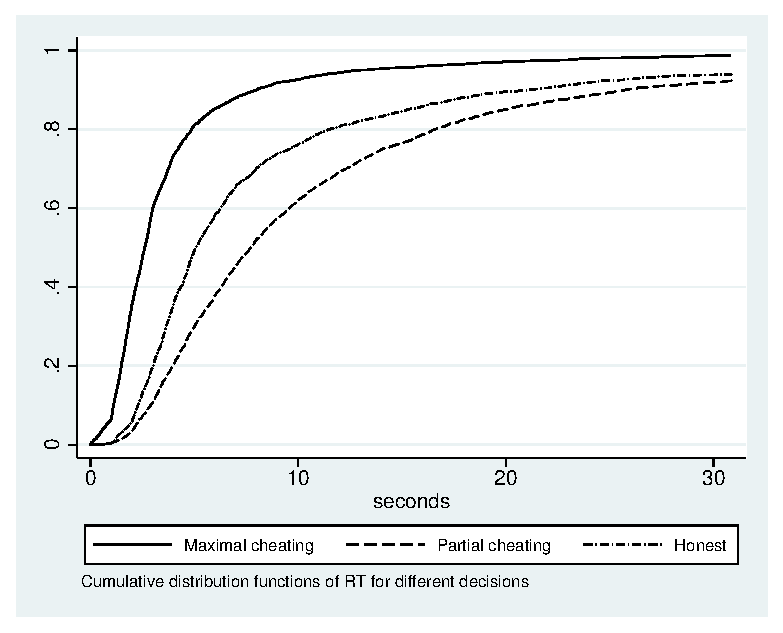
\includegraphics[width=3in]{response.eps}
\label{fig:response}
}
\subfigure[Reaction time depending on fraction declared in the current and previous periods]{
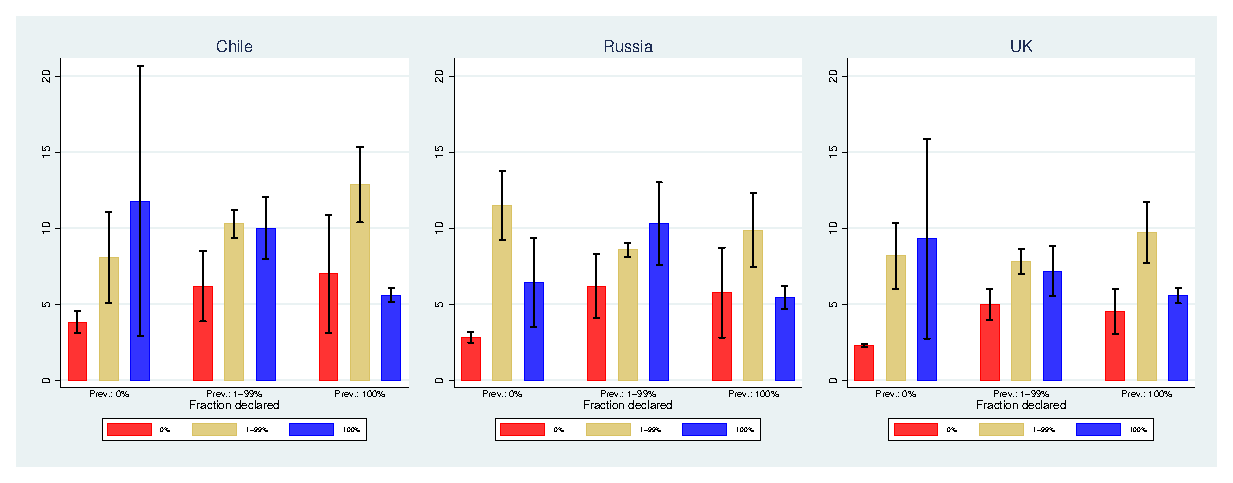
\includegraphics[width=3in]{response_bar.eps}
\label{fig:response_bar}
}
\caption{Reaction time}
\end{figure}
\end{comment}


\begin{figure}[!htb]
\centerline{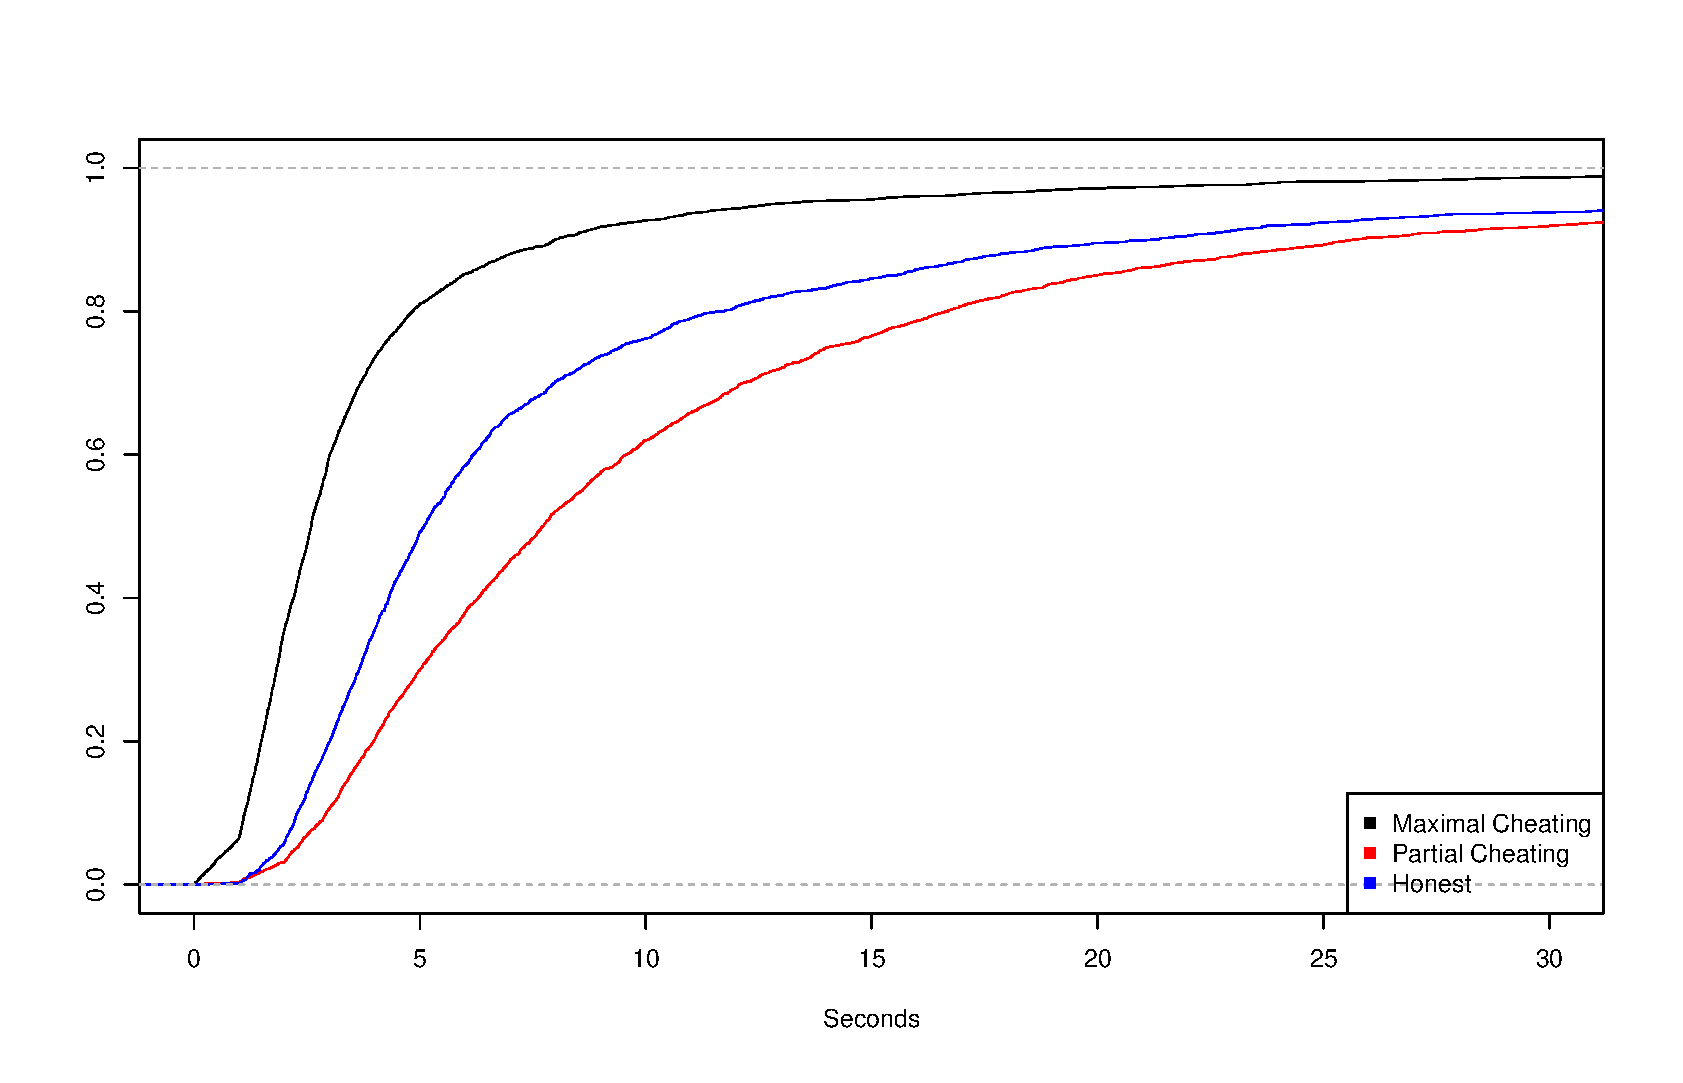
\includegraphics[scale=0.6]{RT_ECDF.eps}}
\caption{Cumulative distributions of reaction times for different declarations}\label{fig:response}
\end{figure}

\par In Table \ref{table_rt} in \ref{AppendixA}, we regress the log reaction time for each decision on individual and treatment controls. In Model 1 we control for the individual's choice, while in Model 2 we also control for the choice made in the previous period, and find that an honest declaration is a much quicker decision than a partial lie. In Model 3 we control for all possible combinations of decisions made in this and previous periods, as well as for decisions made in Period 1. We find that in Period 1, it took more time to declare 100\% of the income than to lie maximally, but less time than to lie partially ($p<0.0001$ on both comparisons); a similar nonlinear relationship between the magnitude of the lie and reaction time was 
present if the subject was honest in the previous period, while a repeated maximal lie took less time than any other type of decision.\footnotemark{}  

\footnotetext{The experimental conditions had some effect on the reaction time. Once the individual's choices are controlled for, the deduction rates and the benefit of lying had no effect; however, the reaction time was higher in the Shock treatment, especially if the subject received unearned income it that period. The reaction time decreased with periods, was shorter for individuals with higher ability at the RET task, and was longer for males and subjects who made higher donations in the dictator game.}

\par The U-shaped relationship between the magnitude of the lie and reaction time suggests two possibilities. First, partial lying necessarily involves a choice from a broad range of alternatives, and hence involves more reflection than either a honest choice or a maximal lie. Second, both noncooperation and honesty can be heuristic responses \citep{Randetal2014,Vershuere2014}, while partial lie involves decision conflict and is slower. 


\section*{Discussion and Conclusion}

\par Individuals lie on a regular basis in their everyday lives, and for many people lying is associated with intrinsic costs that increase with the degree to which the truth is distorted. The goal of this work was to learn more about the nature of these costs. For this goal, we observed over 1,000 individuals from the U.K., Russia and Chile making over 10,000 lying decisions in a public goods game with earned income. We implemented treatments aimed at varying the benefit of lying, as well as several other characteristics of the game, such as whether there was earned as well as unearned income. 

\par We find that both maximal lying (when the subjects maximized their monetary gain) and partial lying were common, as well as honest behavior, and lying was not responsive to externally imposed benefits. This is not consistent with the marginal cost of lying increasing in the magnitude of the lie (in which case one would expect the magnitude of partial lies and/or the incidence of maximal lie to increase with the benefits of lying). 

\par We offer an alternative explanation that partial lying is a result of some subjects have lying thresholds; the intrinsic costs of lying for such individuals are low when the magnitude of the lie is below the threshold. Our experiments suggest that such thresholds are heterogeneous both across individuals and across individual decisions, but are unaffected by extrinsic benefits and other experimental conditions.\footnotemark{}
\footnotetext{This finding is contrary to \cite{Gibsonetal2013} who conclude that the likelihood of lying will vary continuously with the costs and benefits. However, our experiment is different in several important respects. First, we explicitly vary the benefits of lying by assigning subjects to treatments with different deduction rates. In the Status treatment, we also manipulate the amount of income that individuals earn through the real effort task, while in the Shock treatment subjects who receive the bonus have high exogenous costs of not lying. Second, the lying decisions are made with respect to the individual's earned income. Finally, our design involves subjects making repeated decisions.} 

\par These thresholds may be shaped by the concerns about one's social identity; social identity theory argues that people derive intrinsic payoffs from belonging to one or another social category \citep{akerlof2000economics,benabou2011identity}. When the magnitude of lying falls below a threshold value individuals are able to maintain a positive self-image and therefore avoid any intrinsic costs of lying \cite{GinoAriely2016}. Individuals may also care about whether their actions are perceived by other people as dishonest, which may cause partial lying \citep{gneezy2018lying}.  

\par We demonstrate that partial lies and maximal lies are distinct phenomena. First, we observe subjects making multiple potential lying decisions, and find that individuals either lie maximally most of the time, or lie partially most of the time, with relatively few individuals doing a lot of both. In two countries out of three, the individual's choice whether to lie maximally, lie partially, or be honest was not conditional, or was only weakly conditional, on the lying of other individuals in the four-member group.  

\par Second, there are individual characteristics that distinguish between maximal liars on one hand, and partial liars and honest individuals on the other. As has been pointed out elsewhere \citep{DuchSolaz2017}, ability is correlated with lying. Our findings are more nuanced. High-ability individuals are indeed more likely to be maximal liars. However, low ability is positively associated not only with honest behavior, but with partial lying as well. 

\par At the same time, partial lies vary both within and between subjects, while efforts to account for this variation were not particularly successful.  Of particular interest is the fact that variables that account for lying strategies (maximal, partial and honest) do not explain variations in the magnitude of partial lies, and people who tend to engage in near-maximal lying do not share the same characteristics as those who tend to lie to the maximal extent. \footnote{In Table C10 we look at partial lying involving very small declarations of earnings (such as between 1 and 50 ECUs).  Even at these extremes we observe that low ability subjects are more likely to engage in partial lying.} A similar pattern is present when we look at other-regarding preferences. Individuals who made zero donations in the Dictator Game were more likely to be maximal liars and less likely to be partial liars, compared with individuals who donated some positive amount. At the same time, an individual who made a positive donation was more likely to be an honest type, compared with an individual who made a smaller or no donation. 

\par Third, our observations are consistent with the assumption that individuals who lie maximally have very small or zero intrinsic costs of lying. Otherwise, maximal lying should have been less prevalent for lower deduction rates, as some of the individuals with higher intrinsic costs of lying would prefer not to lie maximally when the deduction rate is low. Instead, maximal lying (as well as honest behavior and partial lying) was equally prevalent among all deduction rates in our experiment. 
 
\par Finally, it requires a high reaction time in order to arrive at a partial lying decision, while both honest choices and, especially, maximal lies involve relatively short reaction time. The long reaction time might suggest that partial lying reflects a preference for maintaining one’s positive social identify while at the same time uncertainty about precisely how big a lie would be consistent with such a goal.

\par Both partial and maximal lying occurred in all three of the different national subject pools --- the U.K. Chile and Russia. Moreover, several of the above patterns that characterize lying are present in all three countries: reaction time is lower for maximal lies and honest decisions than for partial lies; ability is positively correlated with maximal lying and negatively --- with partial lies and honesty; people who tend to lie maximally in the public goods game behave similarly in the die tossing game. 

\par National context, though, is not irrelevant.  All three countries in our study exhibit these same three distinct behaviors although their distribution within each country is quite different.  In Chile the modal behavior was predominantly honest --- 40 percent of subjects reported 100 percent of their earnings. In Russia honest behavior was least common, while in the U.K. we saw the highest concentration of maximal liars.  Why they differed is an important puzzle that is beyond the scope of these data but is the focus of our ongoing research. 

\par As we pointed out earlier, the economic costs of lying are enormous.  An important challenge then is simply designing mechanisms for reducing lying both in the public and private sectors. The point of departure should be a good understanding of the lying mechanism.  We make some modest contributions in this respect.  Our experimental results suggest that modifying the extrinsic costs of not lying may have little effect -- this is simply the case because many in the population will lie maximally regardless of the stakes.  

\par Are there appeals to intrinsic motivations that might resonate with the types of lying behavior that we identify in the population?  Possibly, although our efforts were not particularly successful in this regard.  Treatments that manipulated the relationship between effort and income, how income is redistributed and deadweight loss had little effect on lying behavior. We find some evidence that subjects who observed their group members declare a large amount of incomes were less likely to lie maximally. Nevertheless, the effect was present and strong only in one country --- Russia.    

\par Our experimental results illustrate that the distribution of lying strategies can vary quite significantly across national, and perhaps other, contexts. Policies, and the investments necessary, for addressing lying in contexts where honest behavior or partial lying is predominant will differ significantly from those populated primarily by maximal liars. Efforts to address lying must therefore begin by estimating the distribution of lying strategies in the population of interest.  The challenge for future research will be to build on our insights into the heterogeneity of lying behavior in order to understand what moderates lying in the population. 


\pagebreak
\doublespacing
\bibliographystyle{apalike}
\bibliography{dave,pastimes_additions}
\newpage

\setcounter{section}{0}
\renewcommand\thesection{Appendix \Alph{section}}
\renewcommand\thesubsection{\Alph{section}\arabic{subsection}}
\renewcommand\thefigure{\Alph{section}\arabic{figure}}
\renewcommand\thetable{\Alph{section}\arabic{table}}

\section{Experiment design}
\setcounter{table}{0}
\setcounter{figure}{0}
\label{Appendix_Design}


\begin{table}[ht] \centering
\tiny
%\begin{table}[tbp] \centering%
\newcolumntype{C}{>{\centering\arraybackslash}X}
\begin{tabularx}{\textwidth}{lCCCCCCC}
\toprule
\#&Country&Treatment&TaxRate&Subjects&Risk&Realdie& \tabularnewline
\midrule\addlinespace[1.5ex]
1&UK&Baseline&10&24&Yes&No& \tabularnewline
2&UK&Baseline&20&24&Yes&No& \tabularnewline
3&UK&Baseline&30&24&Yes&No& \tabularnewline
4&UK&Baseline&40&24&Yes&No& \tabularnewline
5&UK&Baseline&50&24&Yes&No& \tabularnewline
6&UK&Status&10&24&Yes&No& \tabularnewline
7&UK&Status&20&12&Yes&No& \tabularnewline
8&UK&Status&20&16&Yes&No& \tabularnewline
9&UK&Status&30&20&Yes&No& \tabularnewline
10&UK&Baseline&10&24&Yes&No&30\% of deductions go to two top performers \tabularnewline
11&UK&Baseline&20&20&Yes&No&30\% of deductions go to two top performers \tabularnewline
12&UK&Baseline&30&20&Yes&No&30\% of deductions go to two top performers \tabularnewline
13&UK&Baseline&40&20&Yes&No&30\% of deductions go to two top performers \tabularnewline
14&UK&Baseline&10&24&Yes&No&Only 30\% of deductions are redistributed \tabularnewline
15&UK&Baseline&20&20&Yes&No&Only 30\% of deductions are redistributed \tabularnewline
16&UK&Shock&10&16&Yes&No&100 ECU per answer+1300 ECU bonus \tabularnewline
17&UK&Shock&20&20&Yes&No&100 ECU per answer+1300 ECU bonus \tabularnewline
18&UK&Shock&30&20&Yes&No&100 ECU per answer+1300 ECU bonus \tabularnewline
19&Chile&Shock&10&16&Yes&No&150 ECU per answer+1300 ECU bonus \tabularnewline
20&Chile&Shock&20&20&Yes&No&150 ECU per answer+1300 ECU bonus \tabularnewline
21&Chile&Shock&30&16&Yes&No&150 ECU per answer+1300 ECU bonus \tabularnewline
22&Chile&Status&10&16&Yes&No& \tabularnewline
23&Chile&Status&20&16&Yes&No& \tabularnewline
24&Chile&Status&30&16&Yes&No& \tabularnewline
25&Chile&Baseline&10&12&Yes&No& \tabularnewline
26&Chile&Baseline&20&12&Yes&No& \tabularnewline
27&Chile&Baseline&30&12&Yes&No& \tabularnewline
28&UK&Non-fixed&10&16&Yes&Yes& \tabularnewline
29&UK&Non-fixed&10&16&Yes&Yes& \tabularnewline
30&UK&Non-fixed&10&16&Yes&Yes& \tabularnewline
31&UK&Non-fixed&10&12&Yes&Yes& \tabularnewline
32&UK&Non-fixed&20&12&Yes&Yes& \tabularnewline
33&UK&Non-fixed&30&16&Yes&Yes& \tabularnewline
34&Chile&Non-fixed&10&20&Yes&Yes& \tabularnewline
35&Chile&Non-fixed&20&20&Yes&Yes& \tabularnewline
36&Chile&Non-fixed&30&20&Yes&Yes& \tabularnewline
37&Chile&Non-fixed&10&16&Yes&Yes& \tabularnewline
38&Chile&Non-fixed&20&12&Yes&Yes& \tabularnewline
39&Chile&Non-fixed&30&8&Yes&Yes& \tabularnewline
40&UK&Baseline&10&16&Yes&Yes& \tabularnewline
41&UK&Non-fixed&20&16&Yes&Yes& \tabularnewline
42&UK&Non-fixed&30&12&Yes&Yes& \tabularnewline
43&Chile&Non-fixed&10&20&Yes&Yes& Universidad del Desarrollo\tabularnewline
44&Chile&Non-fixed&10&24&Yes&Yes& Universidad del Desarrollo\tabularnewline
45&Chile&Non-fixed&20&20&Yes&Yes& Universidad del Desarrollo\tabularnewline
46&Chile&Non-fixed&30&20&Yes&Yes& Universidad del Desarrollo\tabularnewline
47&Russia&Baseline&10&8&Yes&No& \tabularnewline
48&Russia&Baseline&10&8&Yes&No& \tabularnewline
49&Russia&Baseline&10&16&Yes&No& \tabularnewline
50&Russia&Baseline&10&16&Yes&No& \tabularnewline
51&Russia&Baseline&20&16&Yes&No& \tabularnewline
52&Russia&Baseline&20&16&Yes&No& \tabularnewline
53&Russia&Baseline&20&8&Yes&No& \tabularnewline
54&Russia&Baseline&20&12&Yes&No& \tabularnewline
55&Russia&Shock&10&16&Yes&Yes&100 ECU per answer+1300 ECU bonus \tabularnewline
56&Russia&Shock&20&16&Yes&Yes&100 ECU per answer+1300 ECU bonus \tabularnewline
57&Russia&Status&10&16&Yes&Yes& \tabularnewline
58&Russia&Status&20&16&Yes&Yes& \tabularnewline
59&Russia&Status&30&16&Yes&Yes& \tabularnewline
60&Russia&Baseline&30&16&Yes&Yes& \tabularnewline
61&Russia&Shock&30&16&Yes&Yes&100 ECU per answer+1300 ECU bonus \tabularnewline
62&Russia&Non-fixed&10&16&Yes&Yes& \tabularnewline
63&Russia&Non-fixed&20&16&Yes&Yes& \tabularnewline
64&Russia&Non-fixed&30&12&Yes&Yes& \tabularnewline
\bottomrule \addlinespace[1.5ex]
\end{tabularx}%
\end{table}%

\begin{tabularx}{\textwidth}{lccccccc}
\toprule
 \tabularnewline
\#&Country&Treatment&Tax rate&Subjects&Risk&Die&Note \tabularnewline
\midrule\addlinespace[1.5ex]
1&U.K.&Baseline&10&24&Yes&No& \tabularnewline
2&U.K.&Baseline&20&24&Yes&No& \tabularnewline
3&U.K.&Baseline&30&24&Yes&No& \tabularnewline
4&U.K.&Baseline&40&24&Yes&No& \tabularnewline
5&U.K.&Baseline&50&24&Yes&No& \tabularnewline
6&U.K.&Status&10&24&Yes&No& \tabularnewline
7&U.K.&Status&20&12&Yes&No& \tabularnewline
8& U.K.&Status&20&16&Yes&No& \tabularnewline
9&U.K.&Status&30&20&Yes&No& \tabularnewline
10&U.K.&Baseline&10&24&Yes&No&30\% of deductions go to two top performers \tabularnewline
11&U.K.&Baseline&20&20&Yes&No&30\% of deductions go to two top performers \tabularnewline
12&U.K.&Baseline&30&20&Yes&No&30\% of deductions go to two top performers \tabularnewline
13&U.K.&Baseline&40&20&Yes&No&30\% of deductions go to two top performers \tabularnewline
14&U.K.&Baseline&10&24&Yes&No&Only 30\% of deductions are redistributed \tabularnewline
15&U.K.&Baseline&20&20&Yes&No&Only 30\% of deductions are redistributed \tabularnewline
16&U.K.&Shock&10&16&Yes&No&100 ECU per answer+1300 ECU bonus \tabularnewline
17&U.K.&Shock&20&20&Yes&No&100 ECU per answer+1300 ECU bonus \tabularnewline
18&U.K.&Shock&30&20&Yes&No&100 ECU per answer+1300 ECU bonus \tabularnewline
19&Chile&Shock&10&16&Yes&No&150 ECU per answer+1300 ECU bonus \tabularnewline
20&Chile&Shock&20&20&Yes&No&150 ECU per answer+1300 ECU bonus, 8 observations invalid \tabularnewline
21&Chile&Shock&30&16&Yes&No&150 ECU per answer+1300 ECU bonus \tabularnewline
22&Chile&Status&10&16&Yes&No& \tabularnewline
23&Chile&Status&20&16&Yes&No& \tabularnewline
24&Chile&Status&30&16&Yes&No& \tabularnewline
25&Chile&Baseline&10&12&Yes&No& \tabularnewline
26&Chile&Baseline&20&12&Yes&No& \tabularnewline
27&Chile&Baseline&30&12&Yes&No& \tabularnewline
28&U.K.&Non-fixed&10&16&Yes&Yes& \tabularnewline
29&U.K.&Non-fixed&10&16&Yes&Yes& \tabularnewline
30&U.K.&Non-fixed&10&16&Yes&Yes& \tabularnewline
31&U.K.&Non-fixed&10&12&Yes&Yes& \tabularnewline
32&U.K.&Non-fixed&20&12&Yes&Yes& \tabularnewline
33&U.K.&Non-fixed&30&16&Yes&Yes& \tabularnewline
34&Chile&Non-fixed&10&20&Yes&Yes& \tabularnewline
35&Chile&Non-fixed&20&20&Yes&Yes& \tabularnewline
36&Chile&Non-fixed&30&20&Yes&Yes& \tabularnewline
37&Chile&Non-fixed&10&16&Yes&Yes& \tabularnewline
38&Chile&Non-fixed&20&12&Yes&Yes& \tabularnewline
39&Chile&Non-fixed&30&8&Yes&Yes& \tabularnewline
40&U.K.&Baseline&10&16&Yes&Yes& \tabularnewline
41&U.K.&Non-fixed&20&16&Yes&Yes& \tabularnewline
42&U.K.&Non-fixed&30&12&Yes&Yes& \tabularnewline
43&Chile&Non-fixed&10&20&Yes&Yes& Universidad del Desarrollo\tabularnewline
44&Chile&Non-fixed&10&24&Yes&Yes& Universidad del Desarrollo\tabularnewline
45&Chile&Non-fixed&20&20&Yes&Yes& Universidad del Desarrollo\tabularnewline
46&Chile&Non-fixed&30&20&Yes&Yes& Universidad del Desarrollo\tabularnewline
47&Russia&Baseline&10&8&Yes&No& \tabularnewline
48&Russia&Baseline&10&8&Yes&No& \tabularnewline
49&Russia&Baseline&10&16&Yes&No& \tabularnewline
50&Russia&Baseline&10&16&Yes&No& \tabularnewline
51&Russia&Baseline&20&16&Yes&No& \tabularnewline
52&Russia&Baseline&20&16&Yes&No& \tabularnewline
53&Russia&Baseline&20&8&Yes&No& \tabularnewline
54&Russia&Baseline&20&12&Yes&No& 30\% of deductions go to two top performers\tabularnewline
55&Russia&Shock&10&16&Yes&Yes&100 ECU per answer+1300 ECU bonus \tabularnewline
56&Russia&Shock&20&16&Yes&Yes&100 ECU per answer+1300 ECU bonus \tabularnewline
57&Russia&Status&10&16&Yes&Yes& \tabularnewline
58&Russia&Status&20&16&Yes&Yes& \tabularnewline
59&Russia&Status&30&16&Yes&Yes& \tabularnewline
60&Russia&Baseline&30&16&Yes&Yes& \tabularnewline
61&Russia&Shock&30&16&Yes&Yes&100 ECU per answer+1300 ECU bonus \tabularnewline
62&Russia&Non-fixed&10&16&Yes&Yes& \tabularnewline
63&Russia&Non-fixed&20&16&Yes&Yes& \tabularnewline
64&Russia&Non-fixed&30&12&Yes&Yes& \tabularnewline
\bottomrule \addlinespace[1.5ex]
\end{tabularx}%

\caption{List of sessions}
\label{tab:sesslist}
\end{table}

\clearpage




\begin{figure}[ht]
\centerline{\includegraphics[width=\textwidth]{english_baseline_module1.eps}}
\caption{Dictator Game}\label{fig:DG}
\end{figure}

\clearpage

\begin{figure}[ht]
\centerline{\includegraphics[width=0.8\textwidth]{english_baseline_module2_intro.eps}}
\caption{On-screen instructions for real effort task, U.K.}
\end{figure}

\vspace{1cm}

\begin{figure}[ht]
\centerline{\includegraphics[width=0.8\textwidth]{english_nonfixed_module2_10_initialpq.eps}}
\caption{Performance prediction before the real effort task, non-fixed treatment, U.K.}
\end{figure}


\clearpage



\begin{figure}[ht]
\centerline{
\includegraphics[width=\textwidth]{ret}}
\caption{Real effort task, U.K.}
\end{figure}
\clearpage

\begin{comment}
\begin{figure}[ht]
\centerline{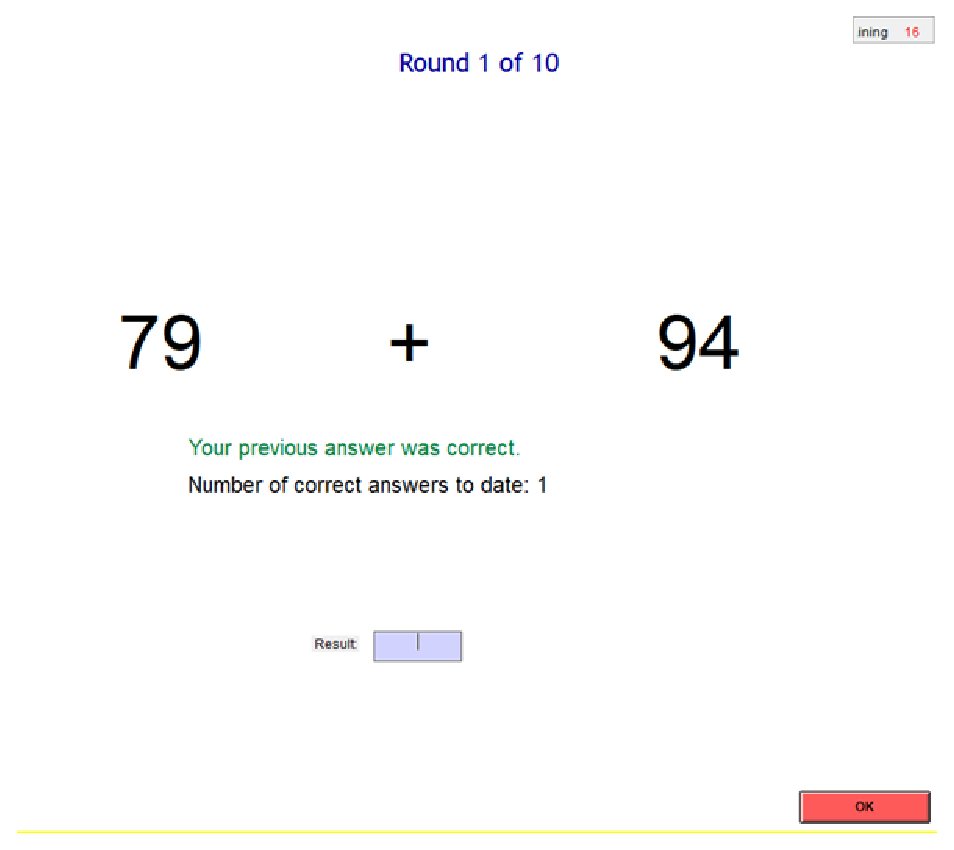
\includegraphics[width=\textwidth]{RETresponse}}
\caption{Real effort task screen with correct answer, U.K.}
\end{figure}
\clearpage
\end{comment}

\begin{figure}[ht]
\centerline{\includegraphics[width=0.8\textwidth]{english_baseline_module2_declare.eps}}
\caption{Declaration of gains following real effort task, U.K.}
\end{figure}

\vspace{1cm}

\begin{figure}[ht]
\centerline{\includegraphics[width=0.8\textwidth]{english_baseline_module2_result.eps}}
\caption{Results following declaration of gains, U.K.}
\end{figure}


\clearpage

\begin{figure}[ht]
\centerline{\includegraphics[width=0.8\textwidth]{english_status_module2_result.eps}}
\caption{Results following declaration of gains, status treatment, U.K.}
\end{figure}

\vspace{1cm}

\begin{figure}[ht]
\centerline{\includegraphics[width=0.8\textwidth]{english_shock_module2_10_result.eps}}
\caption{Results following declaration of gains, shock treatment, U.K.}
\end{figure}

\clearpage


\begin{figure}[ht]
\centerline{\includegraphics[width=0.8\textwidth]{english_baseline_module4_intro.eps}}
\caption{On-screen instructions Risk Aversion questions}
\label{fig:screen_risk1}
\end{figure}

\vspace{1cm}

\begin{figure}[ht]
\centerline{\includegraphics[width=0.8\textwidth]{english_baseline_module4_risk.eps}}
\caption{Risk aversion questions}
\label{fig:screen_risk2}
\end{figure}

\clearpage

\begin{figure}[ht]
\centerline{
\includegraphics[width=\textwidth]{IntroDie}}
\caption{On-screen instructions, Die Game}
\label{fig:diegame}
\end{figure}
\clearpage



\clearpage
\section{Supplemental analysis.}
\subsection{Performance at the real-effort task. }
\setcounter{table}{0}
\setcounter{figure}{0}
\label{subj_peft}

Here, we look at the determinants of performance at the real effort task.  In both Russia and the U.K., the experiment was carried out at elite universities (Higher School of Economics and Oxford, respectively), while in Chile 15/19 sessions were held at the more inclusive Universidad de Santiago and the remaining  4 sessions were held at the elite Universidad del Desarrollo. This is reflected in performance: subjects, on average, complete 8.29 (sd=2.43) additions in Chile, 11.25 (sd=2.59) in Russia, and 11.85 (sd=3.89) in the U.K. All differences between countries are significant ($p=0.0069$ for two-tailed Welch $t$-test comparing average performance in Russia and the U.K., and $p<0.0001$ for all other pairwise comparisons; the distributions of subject performance are plotted on Figure \ref{fig:correct_sums}).\label{stata:ret}


\begin{figure}[!htb]
\centerline{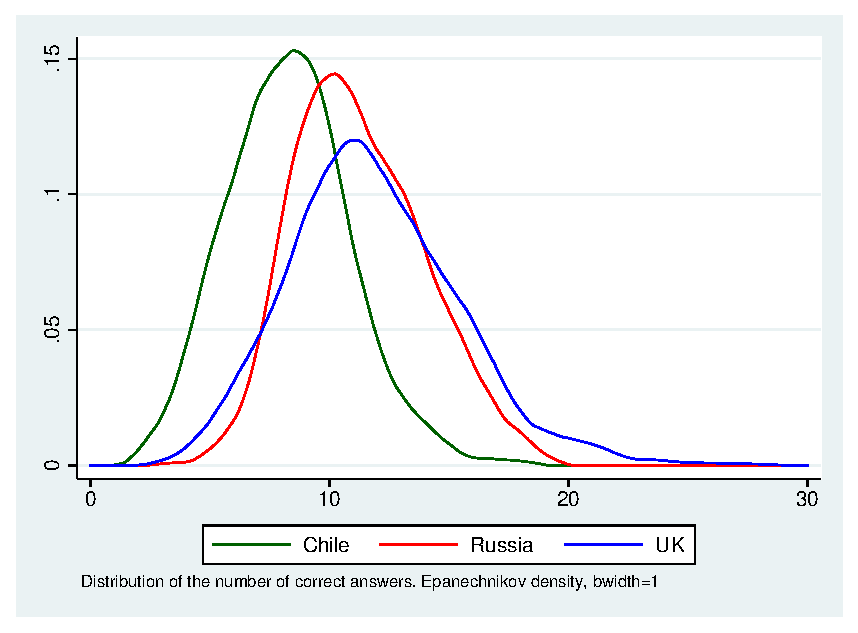
\includegraphics[width=1\textwidth]{ret_density.eps}}
\caption{Distribution of average performance by country}\label{fig:correct_sums}
\end{figure}


%In Russia and the U.K., subjects who donated zero in the Dictator Game had better average performance at the real effort task (by 1.26 and 1.36 correct answers, respectively, with $p=0.0021$ and $p=0.0001$ for two-tailed Welch $t$-test). In Chile the difference was not significant. This is consistent with the broad hypothesis that ability is negatively associated with prosocial behavior.

In Table \ref{table_ret} we provide the results of OLS regressions of subject's average performance. The regression include control variables for Norms, calculated as the normalized first principle component based on ten survey questions regarding the justifiability of certain types of unethical behaviors, such as not paying for public transport (Table \ref{tab:norms} has specific question word). Trust is measured using a standard social capital question on how much a person can trust others. Following \cite{Holtetal2002}, the Safe choices variable is an additive index of ten lottery choices (selecting between two payment options) with increasing probabilities of earning the largest payment options. Ideology is measured using an 11-point Left-Right self-placement scale. Income is a self reported survey question on family income, where higher categories reflect higher income levels, and categories are country specific. The full questionnaire is available in replication code.    

In Russia and the U.K., the Dictator Game donations are negatively associated with the subsequent RET performance, while male subjects rank significantly higher in every country, other individual-level covariates are generally not significant.

\begin{table}[ht]
\scriptsize
\begin{center}
{
\def\sym#1{\ifmmode^{#1}\else\(^{#1}\)\fi}
\begin{tabular}{l*{4}{cc}}
\hline\hline
                &\multicolumn{2}{c}{Chile}   &\multicolumn{2}{c}{Russia}  &\multicolumn{2}{c}{UK}      &\multicolumn{2}{c}{All}     \\
\hline
Male            &    1.597\sym{***}&  (0.313)&    1.457\sym{***}&  (0.309)&    1.096\sym{***}&  (0.345)&    1.302\sym{***}&  (0.195)\\
Age             &  -0.0478         & (0.0304)&  -0.0246         & (0.0404)&   -0.102\sym{***}& (0.0186)&  -0.0981\sym{***}& (0.0146)\\
DG=0            &    0.153         &  (0.817)&    0.218         &  (0.462)&    0.222         &  (0.629)&    0.472         &  (0.356)\\
DG above 0      & 0.000176         &(0.000955)& -0.00214\sym{**} &(0.000952)& -0.00290\sym{**} &(0.00127)& -0.00188\sym{***}&(0.000633)\\
Deduction 20\%  &    0.620\sym{*}  &  (0.343)&    0.435         &  (0.323)&   -0.267         &  (0.418)&    0.267         &  (0.222)\\
Deduction 30\%  &    0.290         &  (0.378)&   0.0145         &  (0.465)&   -0.209         &  (0.444)&   0.0569         &  (0.246)\\
Deduction 40\%  &                  &         &                  &         &    0.334         &  (0.738)&    0.685         &  (0.669)\\
Deduction 50\%  &                  &         &                  &         &    0.502         &  (0.759)&    0.843         &  (0.662)\\
Deadweight loss &                  &         &                  &         &    1.916\sym{***}&  (0.683)&    2.019\sym{***}&  (0.615)\\
Redistribution  &                  &         &                  &         &    0.449         &  (0.585)&    0.650         &  (0.531)\\
Russia          &                  &         &                  &         &                  &         &    2.461\sym{***}&  (0.270)\\
UK              &                  &         &                  &         &                  &         &    3.231\sym{***}&  (0.295)\\
Shock           &    0.553         &  (0.550)&    0.385         &  (0.467)&    1.100\sym{*}  &  (0.612)&    0.680\sym{**} &  (0.302)\\
Status          &    0.961\sym{*}  &  (0.567)&    0.644         &  (0.587)&    0.762         &  (0.624)&    0.667\sym{*}  &  (0.347)\\
Status, 200 ECU &   -0.704         &  (0.620)&   0.0542         &  (0.775)&    0.736         &  (0.829)&    0.125         &  (0.462)\\
Non-fixed       &    1.488\sym{***}&  (0.485)&    1.152\sym{***}&  (0.431)&   -0.498         &  (0.511)&    0.478\sym{*}  &  (0.265)\\
Norms           &   -0.162         &  (0.166)&    0.230         &  (0.147)&    0.358\sym{**} &  (0.172)&    0.217\sym{**} & (0.0940)\\
Trust           &    0.329         &  (0.318)&   -0.478         &  (0.319)&   -0.431         &  (0.347)&   -0.255         &  (0.199)\\
SafeChoices     &  -0.0292         & (0.0867)&   0.0677         & (0.0820)&  -0.0307         & (0.0864)& -0.00340         & (0.0506)\\
Ideology        &   0.0575         & (0.0727)&  -0.0975         & (0.0772)&    0.125\sym{*}  & (0.0730)&   0.0635         & (0.0434)\\
Income          &   -0.342         &  (0.525)&   -0.523         &  (0.805)&   -0.127         &  (0.492)&   -0.176         &  (0.335)\\
Constant        &    7.350\sym{***}&  (1.221)&    11.59\sym{***}&  (1.211)&    14.12\sym{***}&  (1.079)&    9.962\sym{***}&  (0.713)\\
\hline
Observations    &      255         &         &      256         &         &      385         &         &      896         &         \\
\(R^{2}\)       &    0.184         &         &    0.178         &         &    0.191         &         &    0.327         &         \\
\hline\hline
\multicolumn{9}{p{17cm}}{\tiny OLS regression. Robust standard errors. Dependent variable is subject's average performance over 10 rounds. DG frac is the fraction of the 1000 ECU donated in the dictator game. Norms is the social norms index (see Table \ref{tab:norms}). SafeChoices if the number (0-10) of safe choices on the lottery task. Trust is whether the individual answered ``Most people can be trusted'' (versus ``You can't be too careful with people''). Income is the number of the individual's income bracket, rescaled between 0 and 1 (for Chile and the UK), and the individual's perceived income decile, rescaled between 0 and 1 (for Russia).}\\
\multicolumn{9}{l}{\footnotesize \sym{*} \(p<0.10\), \sym{**} \(p<0.05\), \sym{***} \(p<0.01\)}\\
\end{tabular}
}

\end{center}
\caption{Determinants of subject's average performance.}
\label{table_ret}
\end{table}

Experimental treatments generally did not have any effect on average performance of the subjects. Importantly, in the Status treatment, subjects earning 200 ECU per correct answer performed no better than subjects who earned only 100 ECU; this would not have been the case if the subjects were facing an increased marginal cost of effort. Similarly, 
the deduction rate did not have any effect on performance at the real-effort task --- despite the fact that it did not affect the amount of lying. 

In Table \ref{table_ret_per} we regress the number of correct answers in a given period on a set of treatment, individual, and period-level covariates. Performance increases with time, improving every period by an average of 0.14 correct answers over periods 2-10 indicating some potential learning effects. % [AZ!! Learning? CITATIONS!!!!!] I only found this paper "Minimizing Learning Behavior in Experiments with Repeated Real-Effort Tasks" but its a working paper from 2014 and it's not very good. 
Performance is largely unaffected by either previous period's windfall income in the shock treatment (although the coefficient is negative and significant in the combined dataset), or by the income declared by the group members in the previous period. 
\begin{table}[ht]
\scriptsize
\begin{center}
{
\def\sym#1{\ifmmode^{#1}\else\(^{#1}\)\fi}
\begin{tabular}{l*{4}{cc}}
\hline\hline
                &\multicolumn{2}{c}{Chile}   &\multicolumn{2}{c}{Russia}  &\multicolumn{2}{c}{UK}      &\multicolumn{2}{c}{All}     \\
\hline
Male            &    1.601\sym{***}&  (0.316)&    1.489\sym{***}&  (0.304)&    1.222\sym{***}&  (0.361)&    1.349\sym{***}&  (0.202)\\
Age             &  -0.0523\sym{*}  & (0.0289)&  -0.0235         & (0.0414)&  -0.0972\sym{***}& (0.0198)&  -0.0952\sym{***}& (0.0150)\\
Period          &    0.155\sym{***}& (0.0155)&    0.164\sym{***}& (0.0165)&    0.107\sym{***}& (0.0151)&    0.138\sym{***}&(0.00868)\\
DG=0            &    0.281         &  (0.861)&    0.228         &  (0.449)&   0.0729         &  (0.664)&    0.447         &  (0.366)\\
DG above 0      & 0.000439         &(0.000982)& -0.00221\sym{**} &(0.000933)& -0.00309\sym{**} &(0.00134)& -0.00184\sym{***}&(0.000643)\\
Deadweight loss &                  &         &                  &         &    2.389\sym{***}&  (0.796)&    2.173\sym{***}&  (0.627)\\
Redistribution  &                  &         &                  &         &    1.120         &  (0.741)&    0.782         &  (0.504)\\
Russia          &                  &         &                  &         &                  &         &    2.453\sym{***}&  (0.288)\\
UK              &                  &         &                  &         &                  &         &    3.089\sym{***}&  (0.326)\\
Shock           &    0.494         &  (0.572)&    0.606         &  (0.494)&    1.947\sym{***}&  (0.744)&    0.963\sym{***}&  (0.330)\\
L.Shock=Yes     &   -0.172         &  (0.292)&   -0.452\sym{*}  &  (0.264)&   -0.400         &  (0.317)&   -0.342\sym{*}  &  (0.177)\\
Status          &    1.045\sym{*}  &  (0.572)&    0.752         &  (0.557)&    1.409\sym{*}  &  (0.736)&    0.845\sym{**} &  (0.357)\\
Status, 200 ECU &   -0.763         &  (0.622)&  -0.0396         &  (0.748)&    0.767         &  (0.817)&    0.103         &  (0.466)\\
Non-fixed       &    1.640\sym{***}&  (0.489)&    1.231\sym{***}&  (0.424)&   0.0286         &  (0.630)&    0.666\sym{**} &  (0.274)\\
L.Dec. others, 1000&   0.0850         & (0.0861)&   -0.213\sym{*}  &  (0.112)&    0.172         &  (0.111)&   0.0201         & (0.0672)\\
Civicness       &    0.125         &  (0.166)&   -0.240\sym{*}  &  (0.142)&   -0.348\sym{*}  &  (0.188)&   -0.217\sym{**} & (0.0989)\\
Trust           &    0.642\sym{**} &  (0.321)&   -0.516         &  (0.322)&   -0.674\sym{*}  &  (0.364)&   -0.273         &  (0.207)\\
SafeChoices     &  -0.0710         & (0.0856)&   0.0526         & (0.0791)&  -0.0417         & (0.0892)&  0.00575         & (0.0521)\\
Ideology        &   0.0898         & (0.0729)&  -0.0855         & (0.0737)&    0.169\sym{**} & (0.0805)&   0.0875\sym{*}  & (0.0464)\\
Income          &   -0.249         &  (0.546)&   -0.607         &  (0.783)&   -0.243         &  (0.521)&   -0.169         &  (0.354)\\
Constant        &    6.508\sym{***}&  (1.254)&    11.08\sym{***}&  (1.209)&    12.76\sym{***}&  (1.231)&    8.921\sym{***}&  (0.780)\\
\hline
Observations    &     2106         &         &     2304         &         &     2988         &         &     7398         &         \\
\(R^{2}\)       &    0.173         &         &    0.158         &         &    0.181         &         &    0.271         &         \\
\hline\hline
\multicolumn{9}{l}{\footnotesize OLS regressions. Dependent variable is parformance in a round. Standard errors are clustered by subject. DG frac is the fraction of the 1000 ECU donated in the dictator game. Norms is the social norms index (see Table \ref{tab:norms}). SafeChoices if the number (0-10) of safe choices on the lottery task. Income is the number of the individual's income bracket, rescaled between 0 and 1 (for Chile and the UK), and the individual's perceived income decile, rescaled between 0 and 1 (for Russia).}\\
\multicolumn{9}{l}{\footnotesize \sym{*} \(p<0.10\), \sym{**} \(p<0.05\), \sym{***} \(p<0.01\)}\\
\end{tabular}
}

\end{center}
\caption{Determinants of subject's performance, periods 2-10.}
\label{table_ret_per}
\end{table}

Importantly, performance is not negatively associated with social norms. In fact, in Russia and the UK this association is positive. This makes it less likely that the observed association between maximal lying and performance is due to the fact that some subjects participate in the experiment only to earn money, and are more willing to both cheat and exert effort at the real-effort task. In Russia, in the post-experiment survey we also asked a number of questions about 
trusting behavior --- whether the person lends money or belongings or keeps the door open; in 
\cite{glaeser2000measuring} this was a significant predictor of trustworthy behavior in experiments, but in our study these questions ware not associated with either higher or lower performance at the real effort task (Table \ref{table_ret_russia}). Maximal lying was also positively associated with performance in a non-incentivized practice period (Table \ref{table2_country_training}). 

\subsection{Near-maximal lying}
\label{nearmax}

\par In our experiments, subjects sometimes declared positive, but very small amounts of income. We believe that most of such ``near-maximal'' lying is not a chance variation from maximal lying, but driven by the same concerns as partial lying in general --- such as finding justification for self-serving behavior \citep{GinoAriely2016}. This conjecture can be analyzed by comparing the prevalence of partial, maximal, and near-maximal lying among different population groups. Of interest here is whether near-maximal liars tend to share population characteristics with maximal liars or, alternatively, resemble partial liars. Our take on the latter outcome is that near-maximal lying is a form of partial lying -- and that stopping short of maximal lying provides subjects with a self-serving justification for their behavior.  
 
\par Previously, we found that subject ability is positively correlated with maximal lying. In Figure \ref{fig:cheat_hilo} we report the fraction of declarations that were classified as maximal lying, limited lying, and near-maximal, defined as being above 0\% and at or below 20\% of the earnings. In all three countries, near-maximal lying was more prevalent among subjects with below-median performance ($p=0.0003$, $p<0.0001$, and $p=0.0271$ on the Fisher's exact test in Chile, Russia, and the U.K.).
\label{stata:nearmaxfig}

\begin{figure}[!htb]
\centerline{\includegraphics[width=1\textwidth]{FigureB2March2018}}
\caption{Prevalence of lying depending on subject performance}\label{fig:cheat_hilo}
\end{figure}

This result persists if we consider increasingly strict definitions of near-maximal lying. In Table \ref{table:nearmax} in Appendix \ref{Appendix_Design}, we compare the prevalence of small but positive declarations (such as 1-90 ECU, 1-80 ECU, all the way down to 1 ECU) among high and low performance subjects. We find that in all three countries high performers are less likely to engage in near-maximal lying, even if we only consider the declarations as small as between 1 and 30 ECU. In Russia, 1 ECU was declared on 26 occasions, 19 of them by low performers --- a difference significant at $p=0.0282$. Looking at other correlates yields similar results: Near-maximal lying is more prevalent among females (Table \ref{table:nearmax_male}) and those who made positive donations in the Dictator game (Table \ref{table:nearmax_dg}).  


\clearpage



\section{Supplemental tables and figures.}
\label{AppendixA}

\setcounter{table}{0}
\setcounter{figure}{0}

\begin{figure}[!htb]
\centerline{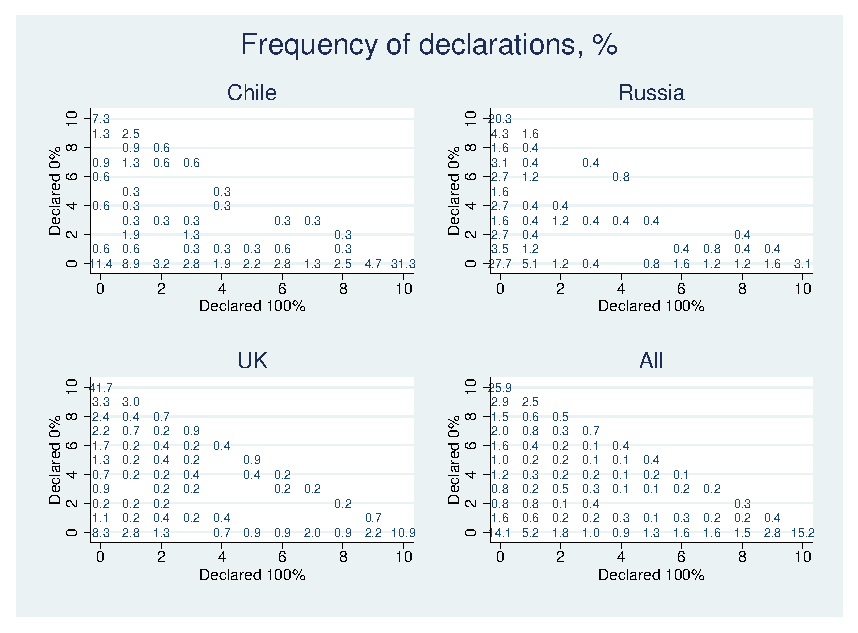
\includegraphics[width=1\textwidth]{declared_freq_all.eps}}
\caption{Frequency of cheating decisions by country. Axis show number of periods.}\label{fig:declared_freq_all}
\end{figure}

\begin{table}[ht]
\begin{center}
\tiny
\def\sym#1{\ifmmode^{#1}\else\(^{#1}\)\fi}
\begin{tabular}{l|cccccccc|cc}
\hline\hline
&\multicolumn{8}{c|}{Mlogit, average marginal effects }&\multicolumn{2}{c}{OLS}\\
                &\multicolumn{2}{c}{Consistent maximal}&\multicolumn{2}{c}{Consistent partial}&\multicolumn{2}{c}{Consistently honest}&\multicolumn{2}{c}{Other}   &\multicolumn{2}{|c}{Partial lying}\\
\hline
RET rank        &    0.194\sym{***}& (0.0382)&  -0.0338         & (0.0349)&  -0.0905\sym{**} & (0.0375)&  -0.0696         & (0.0527)&    0.153\sym{*}  & (0.0805)\\
Male            &   0.0719\sym{***}& (0.0230)&  -0.0839\sym{***}& (0.0204)&  -0.0176         & (0.0212)&   0.0295         & (0.0305)&   0.0178         & (0.0464)\\
Age             & -0.00366         &(0.00231)& -0.00114         &(0.00253)&  0.00138         &(0.00176)&  0.00342         &(0.00309)&  0.00193         &(0.00413)\\
DG=0          &    0.364\sym{***}& (0.0624)&   -0.121\sym{***}& (0.0238)&  -0.0790\sym{**} & (0.0386)&   -0.163\sym{***}& (0.0589)&  -0.0281         & (0.0984)\\
DG frac         &  -0.0494         & (0.0896)&   -0.105\sym{*}  & (0.0588)&    0.216\sym{***}& (0.0689)&  -0.0615         &  (0.101)&    0.222         &  (0.148)\\
Deduction 20\%&  -0.0297         & (0.0271)&   0.0212         & (0.0235)&   0.0237         & (0.0244)&  -0.0152         & (0.0359)&   0.0340         & (0.0447)\\
Deduction 30\%& -0.00436         & (0.0287)&  -0.0355         & (0.0248)&  0.00252         & (0.0258)&   0.0373         & (0.0382)& -0.00567         & (0.0576)\\
Deduction 40\%&  -0.0167         & (0.0570)&  -0.0723         & (0.0483)&  -0.0777         & (0.0488)&    0.167\sym{**} & (0.0806)&    0.150         &  (0.184)\\
Deduction 50\%&   0.0141         & (0.0620)& -0.00678         & (0.0833)&  -0.0600         & (0.0778)&   0.0527         &  (0.117)&   -0.206         &  (0.174)\\
Deadweight loss&  -0.0381         & (0.0513)&  -0.0264         & (0.0514)&   0.0744         & (0.0684)& -0.00991         & (0.0859)&   -0.169         &  (0.129)\\
Redistribution&  0.00253         & (0.0428)&  -0.0439         & (0.0428)&-0.000472         & (0.0577)&   0.0419         & (0.0697)&  -0.0736         &  (0.124)\\
Shock         &-0.000512         & (0.0384)&  -0.0264         & (0.0282)&   0.0246         & (0.0413)&  0.00231         & (0.0513)&  -0.0539         & (0.0642)\\
Status        &   0.0680         & (0.0471)& -0.00285         & (0.0369)&  -0.0197         & (0.0464)&  -0.0454         & (0.0621)& -0.00267         & (0.0709)\\
Status, 200 ECU&  -0.0334         & (0.0493)&  -0.0112         & (0.0425)&   0.0861         & (0.0693)&  -0.0415         & (0.0796)&   0.0154         & (0.0879)\\
Non-fixed     & -0.00140         & (0.0331)&  -0.0708\sym{***}& (0.0261)&   0.0350         & (0.0326)&   0.0371         & (0.0434)&   0.0515         & (0.0565)\\
Russia        &   0.0708\sym{*}  & (0.0419)&   0.0890\sym{**} & (0.0358)&   -0.165\sym{***}& (0.0189)&  0.00524         & (0.0461)&   0.0267         & (0.0510)\\
UK            &    0.259\sym{***}& (0.0358)&  -0.0488\sym{*}  & (0.0287)&   -0.104\sym{***}& (0.0239)&   -0.106\sym{**} & (0.0411)&  -0.0892         & (0.0608)\\
Constant        &                  &         &                  &         &                  &         &                  &         &    0.121         &  (0.128)\\
\hline
Observations    &     1072         &         &     1072         &         &     1072         &         &     1072         &         &      148         &         \\
D20=D30         &    0.383         &         &   0.0293         &         &    0.436         &         &    0.183         &         &    0.480         &         \\
D20=D40         &    0.821         &         &   0.0638         &         &   0.0451         &         &   0.0262         &         &    0.533         &         \\
D20=D50         &    0.482         &         &    0.736         &         &    0.285         &         &    0.564         &         &    0.172         &         \\
D30=D40         &    0.832         &         &    0.475         &         &    0.116         &         &    0.120         &         &    0.419         &         \\
D30=D50         &    0.769         &         &    0.735         &         &    0.433         &         &    0.897         &         &    0.267         &         \\
D40=D50         &    0.685         &         &    0.475         &         &    0.843         &         &    0.397         &         &    0.152         &         \\
Russia=UK       & 1.70e-08         &         &0.00000972         &         &   0.0130         &         &  0.00829         &         &   0.0366         &         \\
\hline\hline
\multicolumn{11}{p{16.5cm}}{\tiny The first four columns report average marginal effects for multinomial logistic regression (the dependent variable is whether the subject was a maximal liar, partial liar, or honest, in all 10 rounds). Robust standard errors. The fifth column reports OLS regression, the dependent variable is the fraction of income declared, averaged across all rounds, for subjects who lied partially in every round. RET rank is the national rank, between 0 and 1, of subject's national performance at the real effort task. RET Deviation is the difference between actual number of correct additions and one predicted from subject and period FE. DG frac is the fraction of the 1000 ECU donated in the dictator game.}\\
\multicolumn{11}{l}{\tiny \sym{*} \(p<0.1\), \sym{**} \(p<0.05\), \sym{***} \(p<0.01\)}\\
\end{tabular}
\end{center}
\caption{Determinants of lying, alternative categorization of subject behavior}
\label{table1_1}
\end{table}

\begin{table}[ht]
\begin{center}
\begin{tabular}{|p{8cm}|cccc|}
\hline
&\multicolumn{4}{c|}{Predicted rank in Period 1}\\
&1&2&3&4\\
\hline
Consistent maximal&   43    	&     35  	&       17  &        5 \\
                  &    47.8\%	&  25.4\%	&   17.2\% &   17.2\%\\ 
Consistent partial&        12  	&       31  &       26 &         7 \\
                  &     13.3\%	&     22.5\%&      26.3\%&      24.1\% \\
 Consistent honest&        21 	&        42 &    32 &         9\\
                  &     23.3\%	&    30.4\%	&      32.3\%&      31.0\% \\
             Other&        14   &     30   	&      24   &       8\\
                  &     15.6\%	&    21.7\%	&     23.2\%&      27.6\%\\
\hline
Total  		&        90  &      138  &       99  &       29\\
Mean rank within one's group, period 1 (sd)&  2.03  (1.06)&	2.49  (1.01)&  2.74 (1.07) & 3.21 (1.01) \\
 $p$-value for two-tailed Welch $t$-test& 0.0016&0.0681&0.0350&\\
\hline
\end{tabular}
\end{center}
\caption{Predicted rank and actual rank in the first period and prevalence of cheating behaviors. Comparisons are of average group rank of subjects with a given predicted rank, and the average group rank of subjects with the next predicted rank. All other pairwise comparisons are significant at $p<0.001$.}
\label{table:init_pred}
\end{table}

\begin{table}[ht]
\begin{center}
\small
{
\def\sym#1{\ifmmode^{#1}\else\(^{#1}\)\fi}
\begin{tabular}{l*{6}{c}}
\hline\hline
                &\multicolumn{1}{c}{1}&\multicolumn{1}{c}{2}&\multicolumn{1}{c}{3}&\multicolumn{1}{c}{4}&\multicolumn{1}{c}{5}&\multicolumn{1}{c}{6}\\
\hline
Type: Consistent maximal liar&  -0.0781\sym{*}  &  -0.0721\sym{*}  &  -0.0244         &   0.0104         &   -0.128\sym{**} &    0.224\sym{***}\\
                & (0.0405)         & (0.0409)         & (0.0356)         & (0.0485)         & (0.0640)         & (0.0618)         \\
Type: Consistent partial liar&   0.0398         &  -0.0148         &  -0.0840         & -0.00898         &   0.0124         &   0.0684         \\
                & (0.0368)         & (0.0406)         & (0.0529)         & (0.0607)         & (0.0790)         & (0.0870)         \\
Av. fraction, partial liars&  -0.0886         &   0.0435         &    0.114         &    0.106         &   0.0428         &   -0.271\sym{*}  \\
                & (0.0774)         & (0.0657)         & (0.0842)         & (0.0963)         &  (0.138)         &  (0.164)         \\
Type: Other     &  -0.0113         &  -0.0300         &  -0.0821\sym{*}  &   0.0786\sym{*}  &   0.0708         &  -0.0433         \\
                & (0.0298)         & (0.0322)         & (0.0439)         & (0.0424)         & (0.0572)         & (0.0662)         \\
Russia          &  -0.0265         &  -0.0618\sym{**} & 0.000537         &  -0.0154         &   0.0200         &   0.0733         \\
                & (0.0295)         & (0.0312)         & (0.0322)         & (0.0347)         & (0.0498)         & (0.0553)         \\
UK              &   0.0204         &  -0.0384         &  -0.0146         &  -0.0734\sym{*}  &  -0.0334         &    0.134\sym{**} \\
                & (0.0277)         & (0.0315)         & (0.0337)         & (0.0422)         & (0.0553)         & (0.0570)         \\
\hline
Observations    &      468         &      468         &      468         &      468         &      468         &      468         \\
\hline\hline
\multicolumn{7}{l}{\footnotesize Logistic regression, marginal coefficients. Individual controls not shown. Average fraction declared is shown for partial liars}\\
\multicolumn{7}{l}{\footnotesize \sym{*} \(p<0.10\), \sym{**} \(p<0.05\), \sym{***} \(p<0.01\)}\\
\end{tabular}
}

\end{center}
\caption{Logit regression of die roll values}
\label{table_dieroll_pred}
\end{table}


\begin{figure}[!htb]
\centerline{\includegraphics[width=1\textwidth]{cheater_type_dgofferMarch2018}}
\caption{Distributions of behavior by Dictator Game donations.}\label{fig:ind_typenew2_dg0}
\end{figure}


\clearpage
\begin{table}[ht]
\begin{center}
\tiny
\def\sym#1{\ifmmode^{#1}\else\(^{#1}\)\fi}
\begin{tabular}{l|cccccc|cc}
\hline\hline
&\multicolumn{6}{c|}{\bf Chile}&\multicolumn{2}{c}{\bf Chile}\\ &\multicolumn{6}{c|}{Mlogit, average marginal effects }&\multicolumn{2}{c}{OLS}\\
                &\multicolumn{2}{c}{Maximal lying}&\multicolumn{2}{c}{Partial lying}&\multicolumn{2}{c|}{Honest}  &\multicolumn{2}{c}{Partial lying}\\
\hline
RET rank        &    0.214\sym{***}& (0.0664)&   -0.127         & (0.0792)&  -0.0866         & (0.0876)&   0.0176         &  (0.136)\\
RET deviation   & -0.00261         &(0.00235)&  0.00421         &(0.00359)& -0.00160         &(0.00354)&   0.0132\sym{**} &(0.00637)\\
Male            &   0.0563         & (0.0380)&  -0.0163         & (0.0477)&  -0.0400         & (0.0512)&    0.112\sym{*}  & (0.0615)\\
Age             &  0.00188         &(0.00254)& -0.00680\sym{*}  &(0.00388)&  0.00492         &(0.00460)&  0.00204         &(0.00549)\\
Period          &  0.00929\sym{***}&(0.00185)& 0.000908         &(0.00258)&  -0.0102\sym{***}&(0.00262)& -0.00311         &(0.00394)\\
DG=0          &    0.406\sym{***}&  (0.146)&   -0.215\sym{**} & (0.0876)&   -0.191         &  (0.141)& -0.00608         &  (0.105)\\
DG frac         &  -0.0695         &  (0.126)&   -0.276\sym{**} &  (0.132)&    0.346\sym{**} &  (0.160)&    0.268         &  (0.228)\\
Deduction 20\%&  -0.0839\sym{**} & (0.0378)&  -0.0770         & (0.0512)&    0.161\sym{***}& (0.0561)&  -0.0173         & (0.0706)\\
Deduction 30\%&   0.0230         & (0.0397)&  -0.0903\sym{*}  & (0.0477)&   0.0673         & (0.0550)&   0.0680         & (0.0747)\\
Shock         &    0.105         &  (0.127)&   0.0413         &  (0.103)&   -0.146         & (0.0931)&    0.172\sym{*}  & (0.0932)\\
Shock, yes    &   0.0111         & (0.0277)&  0.00132         & (0.0441)&  -0.0124         & (0.0427)&  -0.0118         & (0.0603)\\
Status        &    0.161         &  (0.153)&   0.0183         &  (0.114)&   -0.179\sym{*}  &  (0.108)&   0.0263         &  (0.118)\\
Status, 200 ECU&  -0.0607         & (0.0664)&  -0.0816         & (0.0910)&    0.142         &  (0.110)&    0.137         &  (0.123)\\
Non-fixed     &    0.155\sym{*}  & (0.0826)&   -0.129         & (0.0798)&  -0.0258         & (0.0771)&    0.139         & (0.0952)\\
Constant        &                  &         &                  &         &                  &         &   0.0821         &  (0.210)\\
\hline
Observations    &     3078         &         &     3078         &         &     3078         &         &      718         &         \\
D20=D30         &   0.0140         &         &    0.810         &         &    0.129         &         &    0.180         &         \\
\hline\hline
&\multicolumn{6}{c|}{\bf Russia}&\multicolumn{2}{c}{\bf Russia}\\ &\multicolumn{6}{c|}{Mlogit, average marginal effects }&\multicolumn{2}{c}{OLS}\\
                &\multicolumn{2}{c}{Maximal lying}&\multicolumn{2}{c}{Partial lying}&\multicolumn{2}{c|}{Honest}  &\multicolumn{2}{c}{Partial lying}\\
\hline
RET rank        &    0.178\sym{**} & (0.0780)&  -0.0893         & (0.0812)&  -0.0883         & (0.0643)&    0.207\sym{**} & (0.0896)\\
RET deviation   & 0.000818         &(0.00364)&  0.00711\sym{*}  &(0.00384)& -0.00793\sym{***}&(0.00296)&  0.00179         &(0.00382)\\
Male            &   0.0402         & (0.0453)&   -0.149\sym{***}& (0.0464)&    0.108\sym{***}& (0.0345)&   0.0133         & (0.0507)\\
Age             &  -0.0187         & (0.0129)&   0.0165         & (0.0106)&  0.00220         &(0.00497)&  0.00205         &(0.00395)\\
Period          &   0.0189\sym{***}&(0.00287)&  -0.0225\sym{***}&(0.00295)&  0.00361\sym{*}  &(0.00205)&  -0.0233\sym{***}&(0.00302)\\
DG=0          &    0.305\sym{***}&  (0.103)&   -0.357\sym{***}& (0.0744)&   0.0524         & (0.0753)&  -0.0620         & (0.0812)\\
DG frac         &   -0.280         &  (0.187)&   0.0635         &  (0.155)&    0.216\sym{**} &  (0.100)&    0.235         &  (0.147)\\
Deduction 20\%&  -0.0801         & (0.0493)&    0.115\sym{**} & (0.0510)&  -0.0349         & (0.0338)&  0.00202         & (0.0530)\\
Deduction 30\%& -0.00589         & (0.0637)&   0.0407         & (0.0633)&  -0.0348         & (0.0381)&  -0.0670         & (0.0646)\\
Shock         &  0.00668         & (0.0719)&  -0.0617         & (0.0638)&   0.0550         & (0.0640)&  -0.0982\sym{*}  & (0.0557)\\
Shock, yes    &  -0.0151         & (0.0430)&   0.0318         & (0.0414)&  -0.0167         & (0.0325)&   0.0112         & (0.0434)\\
Status        &  -0.0282         & (0.0879)&  -0.0304         & (0.0943)&   0.0586         & (0.0700)&  -0.0448         & (0.0593)\\
Status, 200 ECU&   0.0206         &  (0.104)&  -0.0538         &  (0.111)&   0.0332         & (0.0906)&  0.00608         & (0.0852)\\
Non-fixed     &   0.0305         & (0.0714)&   -0.127\sym{*}  & (0.0656)&   0.0962\sym{*}  & (0.0578)&  0.00157         & (0.0835)\\
Constant        &                  &         &                  &         &                  &         &    0.296\sym{***}&  (0.113)\\
\hline
Observations    &     2560         &         &     2560         &         &     2560         &         &     1012         &         \\
D20=D30         &    0.239         &         &    0.240         &         &    0.997         &         &    0.272         &         \\
\hline\hline
&\multicolumn{6}{c|}{\bf UK}&\multicolumn{2}{c}{\bf UK}\\ &\multicolumn{6}{c|}{Mlogit, average marginal effects }&\multicolumn{2}{c}{OLS}\\
                &\multicolumn{2}{c}{Maximal lying}&\multicolumn{2}{c}{Partial lying}&\multicolumn{2}{c|}{Honest}  &\multicolumn{2}{c}{Partial lying}\\
\hline
RET rank        &    0.368\sym{***}& (0.0493)&  -0.0665         & (0.0475)&   -0.301\sym{***}& (0.0522)&   0.0118         &  (0.124)\\
RET deviation   & -0.00114         &(0.00212)&  0.00223         &(0.00239)& -0.00109         &(0.00189)& -0.00425         &(0.00523)\\
Male            &   0.0857\sym{***}& (0.0319)&   -0.120\sym{***}& (0.0276)&   0.0343         & (0.0286)&  -0.0165         & (0.0707)\\
Age             & -0.00729\sym{***}&(0.00236)&  0.00474\sym{**} &(0.00208)&  0.00255         &(0.00205)&  0.00154         &(0.00415)\\
Period          &   0.0210\sym{***}&(0.00206)&  -0.0106\sym{***}&(0.00195)&  -0.0104\sym{***}&(0.00162)&  -0.0157\sym{***}&(0.00323)\\
DG=0          &    0.348\sym{***}& (0.0511)&   -0.233\sym{***}& (0.0332)&   -0.115\sym{***}& (0.0426)&   0.0303         &  (0.111)\\
DG frac         &   -0.134         &  (0.102)&   -0.207\sym{**} & (0.0883)&    0.340\sym{***}& (0.0982)&    0.481\sym{*}  &  (0.250)\\
Deduction 20\%&   0.0150         & (0.0393)&   0.0306         & (0.0358)&  -0.0456         & (0.0303)&   0.0535         & (0.0768)\\
Deduction 30\%&   0.0699\sym{*}  & (0.0406)&  -0.0469         & (0.0343)&  -0.0230         & (0.0357)&   0.0871         &  (0.105)\\
Deduction 40\%&-0.000970         & (0.0645)&   0.0634         & (0.0594)&  -0.0625         & (0.0457)&    0.202\sym{*}  &  (0.108)\\
Deduction 50\%&    0.100         & (0.0771)&   0.0118         & (0.0741)&   -0.112\sym{**} & (0.0472)&   -0.307\sym{***}&  (0.104)\\
Deadweight loss&  -0.0937         & (0.0631)&  0.00492         & (0.0560)&   0.0887         & (0.0569)&  -0.0983         &  (0.133)\\
Redistribution&   0.0491         & (0.0520)&  -0.0148         & (0.0440)&  -0.0342         & (0.0440)&   -0.130         &  (0.108)\\
Shock         &  0.00231         & (0.0604)&  -0.0262         & (0.0550)&   0.0239         & (0.0567)&   -0.200\sym{**} & (0.0904)\\
Shock, yes    &  -0.0351         & (0.0390)&   0.0823\sym{*}  & (0.0452)&  -0.0472         & (0.0287)&  -0.0442\sym{**} & (0.0220)\\
Status        &    0.140\sym{**} & (0.0658)&  -0.0589         & (0.0635)&  -0.0807         & (0.0549)&  -0.0969         &  (0.149)\\
Status, 200 ECU&   -0.151\sym{*}  & (0.0820)& 0.000806         & (0.0958)&    0.150         &  (0.115)&  -0.0369         &  (0.138)\\
Non-fixed     &  -0.0326         & (0.0474)&   0.0529         & (0.0437)&  -0.0203         & (0.0378)&  -0.0452         &  (0.106)\\
Constant        &                  &         &                  &         &                  &         &    0.224         &  (0.152)\\
\hline
Observations    &     5080         &         &     5080         &         &     5080         &         &      661         &         \\
D20=D30         &    0.206         &         &   0.0410         &         &    0.556         &         &    0.687         &         \\
D20=D40         &    0.809         &         &    0.571         &         &    0.719         &         &    0.132         &         \\
D20=D50         &    0.284         &         &    0.800         &         &    0.189         &         & 0.000685         &         \\
D30=D40         &    0.288         &         &   0.0672         &         &    0.427         &         &    0.368         &         \\
D30=D50         &    0.703         &         &    0.438         &         &    0.106         &         &  0.00408         &         \\
D40=D50         &    0.239         &         &    0.519         &         &    0.389         &         &0.00000483         &         \\
\hline\hline
\multicolumn{9}{p{16cm}}{\tiny The first three columns report average marginal effects for multinomial logistic regression (dependent variable is whether the subject declared 0\%, 100\%, or something in between, in a given round). Standard errors are clustered by subject. The fourth column reports OLS regression, the dependent variable is the fraction of income declared in a given round. We only include subjects who partially cheated in at least 8 rounds, and declarations strictly between 0\% and 100\%. Standard errors are clustered by subject. RET rank is the national rank, between 0 and 1, of subject's national performance at the real effort task. RET Deviation is the difference between actual number of correct additions and one predicted from subject and period FE. DG frac is the fraction of the 1000 ECU donated in the dictator game.}\\
\multicolumn{9}{l}{\tiny \sym{*} \(p<0.1\), \sym{**} \(p<0.05\), \sym{***} \(p<0.01\)}\\
\end{tabular}
\end{center}
\caption{Determinants of lying in each period, by country}
\label{table2_country}
\end{table}

\clearpage
\begin{table}[ht]
\begin{center}
\tiny
\def\sym#1{\ifmmode^{#1}\else\(^{#1}\)\fi}
\begin{tabular}{l|cccccc|cc}
\hline\hline
&\multicolumn{6}{c|}{\bf All\space{}countries,\space{}females}&\multicolumn{2}{c}{\bf All\space{}countries,\space{}females}\\ &\multicolumn{6}{c|}{Mlogit, average marginal effects }&\multicolumn{2}{c}{OLS}\\
                &\multicolumn{2}{c}{Maximal lying}&\multicolumn{2}{c}{Partial lying}&\multicolumn{2}{c}{Honest}  &\multicolumn{2}{c}{Partial lying}\\
\hline
RET rank        &    0.265\sym{***}& (0.0500)&   -0.141\sym{**} & (0.0583)&   -0.124\sym{**} & (0.0573)&   0.0662         & (0.0800)\\
RET deviation   & -0.00435\sym{**} &(0.00214)&  0.00779\sym{***}&(0.00275)& -0.00344         &(0.00234)&-0.000737         &(0.00334)\\
Age             & -0.00819\sym{**} &(0.00331)&  0.00248         &(0.00366)&  0.00571\sym{**} &(0.00288)&  0.00599         &(0.00400)\\
Period          &   0.0175\sym{***}&(0.00191)& -0.00946\sym{***}&(0.00210)& -0.00802\sym{***}&(0.00177)&  -0.0168\sym{***}&(0.00246)\\
DG=0=1          &    0.403\sym{***}& (0.0731)&   -0.357\sym{***}& (0.0398)&  -0.0462         & (0.0696)& -0.00457         & (0.0779)\\
DG frac         &   -0.156         &  (0.103)&   -0.251\sym{**} &  (0.119)&    0.406\sym{***}&  (0.122)&    0.239\sym{*}  &  (0.132)\\
Deduction 20\%=1&  -0.0257         & (0.0342)&  -0.0182         & (0.0390)&   0.0439         & (0.0354)&  -0.0107         & (0.0461)\\
Deduction 30\%=1&   0.0227         & (0.0389)&  -0.0549         & (0.0407)&   0.0322         & (0.0388)&  -0.0199         & (0.0502)\\
Deduction 40\%=1&  -0.0108         & (0.0640)&   0.0368         & (0.0820)&  -0.0260         & (0.0777)&    0.280\sym{***}& (0.0997)\\
Deduction 50\%=1&    0.130         &  (0.117)&    0.102         &  (0.120)&   -0.231\sym{***}& (0.0443)&   -0.219\sym{***}& (0.0633)\\
Deadweight loss=1&   -0.125\sym{**} & (0.0531)&    0.115         & (0.0969)&  0.00960         & (0.0890)&   0.0123         &  (0.132)\\
Redistribution=1&   0.0237         & (0.0503)&   0.0432         & (0.0636)&  -0.0668         & (0.0612)& -0.00215         & (0.0809)\\
Russia=1        &   0.0650         & (0.0490)&    0.220\sym{***}& (0.0516)&   -0.285\sym{***}& (0.0301)&   0.0251         & (0.0546)\\
UK=1            &    0.225\sym{***}& (0.0446)&  -0.0673         & (0.0467)&   -0.157\sym{***}& (0.0361)&  -0.0595         & (0.0565)\\
Shock=1         &  -0.0284         & (0.0483)&   0.0869         & (0.0636)&  -0.0585         & (0.0568)&  -0.0973\sym{*}  & (0.0508)\\
Shock, yes=1    &  -0.0269         & (0.0253)&   0.0185         & (0.0378)&  0.00839         & (0.0349)&   0.0310         & (0.0383)\\
Status=1        &  -0.0271         & (0.0567)&    0.131\sym{*}  & (0.0739)&   -0.104\sym{*}  & (0.0617)&  -0.0196         & (0.0622)\\
Status, 200 ECU=1&  -0.0528         & (0.0608)&  -0.0957         & (0.0777)&    0.148\sym{*}  & (0.0879)&   0.0215         & (0.0712)\\
Non-fixed=1     &  -0.0810\sym{*}  & (0.0426)&   0.0647         & (0.0517)&   0.0162         & (0.0453)&   0.0491         & (0.0618)\\
Constant        &                  &         &                  &         &                  &         &    0.185         &  (0.135)\\
\hline
Observations    &     5220         &         &     5220         &         &     5220         &         &     1545         &         \\
D20=D30         &    0.200         &         &    0.398         &         &    0.772         &         &    0.849         &         \\
D20=D40         &    0.816         &         &    0.496         &         &    0.353         &         &  0.00225         &         \\
D20=D50         &    0.182         &         &    0.322         &         &0.000000159         &         & 0.000430         &         \\
D30=D40         &    0.616         &         &    0.274         &         &    0.461         &         &  0.00314         &         \\
D30=D50         &    0.363         &         &    0.200         &         &0.00000261         &         &  0.00254         &         \\
D40=D50         &    0.244         &         &    0.625         &         &   0.0140         &         &0.000000147         &         \\
Russia=UK       & 0.000109         &         & 1.77e-10         &         & 0.000433         &         &    0.102         &         \\
\hline\hline
&\multicolumn{6}{c|}{\bf All\space{}countries,\space{}males}&\multicolumn{2}{c}{\bf All\space{}countries,\space{}males}\\ &\multicolumn{6}{c|}{Mlogit, average marginal effects }&\multicolumn{2}{c}{OLS}\\
                &\multicolumn{2}{c}{Maximal lying}&\multicolumn{2}{c}{Partial lying}&\multicolumn{2}{c}{Honest}  &\multicolumn{2}{c}{Partial lying}\\
\hline
RET rank        &    0.301\sym{***}& (0.0504)&  -0.0871\sym{*}  & (0.0498)&   -0.214\sym{***}& (0.0513)&    0.104         &  (0.117)\\
RET deviation   &  0.00179         &(0.00206)& 0.000568         &(0.00233)& -0.00236         &(0.00209)&   0.0106\sym{**} &(0.00530)\\
Age             & -0.00364         &(0.00237)&  0.00198         &(0.00214)&  0.00166         &(0.00207)&-0.000138         &(0.00418)\\
Period          &   0.0169\sym{***}&(0.00180)&  -0.0109\sym{***}&(0.00184)& -0.00599\sym{***}&(0.00160)&  -0.0124\sym{***}&(0.00357)\\
DG=0=1          &    0.267\sym{***}& (0.0634)&   -0.158\sym{***}& (0.0424)&   -0.108\sym{**} & (0.0508)&  -0.0419         & (0.0918)\\
DG frac         &   -0.220\sym{**} &  (0.110)&  -0.0335         & (0.0801)&    0.253\sym{***}& (0.0881)&    0.286         &  (0.203)\\
Deduction 20\%=1&  -0.0609\sym{*}  & (0.0367)&   0.0624\sym{*}  & (0.0357)& -0.00155         & (0.0345)&  -0.0122         & (0.0686)\\
Deduction 30\%=1&   0.0456         & (0.0395)&  -0.0162         & (0.0350)&  -0.0294         & (0.0353)&   0.0161         & (0.0813)\\
Deduction 40\%=1&  -0.0399         & (0.0877)&    0.115         & (0.0847)&  -0.0749         & (0.0663)&    0.105         &  (0.150)\\
Deduction 50\%=1&   0.0387         & (0.0866)& -0.00360         &  (0.107)&  -0.0351         & (0.0943)&   -0.346\sym{***}&  (0.124)\\
Deadweight loss=1&  -0.0132         & (0.0778)&   -0.122\sym{*}  & (0.0634)&    0.135\sym{*}  & (0.0772)&   -0.253\sym{*}  &  (0.146)\\
Redistribution=1&   0.0691         & (0.0676)&  -0.0542         & (0.0573)&  -0.0148         & (0.0673)&   -0.131         &  (0.197)\\
Russia=1        &    0.151\sym{***}& (0.0421)&  0.00630         & (0.0372)&   -0.157\sym{***}& (0.0334)&  -0.0718         & (0.0659)\\
UK=1            &    0.376\sym{***}& (0.0391)&   -0.215\sym{***}& (0.0364)&   -0.161\sym{***}& (0.0364)&   -0.102         &  (0.106)\\
Shock=1         &   0.0321         & (0.0527)&  -0.0561         & (0.0405)&   0.0241         & (0.0526)&   0.0284         & (0.0768)\\
Shock, yes=1    &  0.00479         & (0.0323)&   0.0397         & (0.0316)&  -0.0445         & (0.0289)&  -0.0724         & (0.0489)\\
Status=1        &    0.150\sym{***}& (0.0578)&   -0.114\sym{**} & (0.0485)&  -0.0359         & (0.0533)&   -0.142         &  (0.114)\\
Status, 200 ECU=1&  -0.0889         & (0.0749)&   0.0318         & (0.0781)&   0.0571         & (0.0875)&    0.171         &  (0.147)\\
Non-fixed=1     &    0.112\sym{***}& (0.0401)&   -0.136\sym{***}& (0.0344)&   0.0240         & (0.0399)&   0.0171         & (0.0904)\\
Constant        &                  &         &                  &         &                  &         &    0.375\sym{**} &  (0.179)\\
\hline
Observations    &     5498         &         &     5498         &         &     5498         &         &      846         &         \\
D20=D30         &  0.00878         &         &   0.0289         &         &    0.466         &         &    0.703         &         \\
D20=D40         &    0.813         &         &    0.532         &         &    0.286         &         &    0.419         &         \\
D20=D50         &    0.259         &         &    0.539         &         &    0.726         &         &  0.00154         &         \\
D30=D40         &    0.341         &         &    0.124         &         &    0.506         &         &    0.565         &         \\
D30=D50         &    0.938         &         &    0.908         &         &    0.953         &         &  0.00592         &         \\
D40=D50         &    0.484         &         &    0.340         &         &    0.700         &         &  0.00197         &         \\
Russia=UK       &0.000000176         &         & 1.64e-09         &         &    0.917         &         &    0.781         &         \\
\hline\hline
\multicolumn{9}{p{16cm}}{\tiny }\\
\multicolumn{9}{l}{\tiny \sym{*} \(p<0.1\), \sym{**} \(p<0.05\), \sym{***} \(p<0.01\)}\\
\end{tabular}
\end{center}
\caption{Determinants of lying in each period, by gender}
\label{table2_gender}
\end{table}


\clearpage
\begin{table}[ht]
\begin{center}
\tiny
\def\sym#1{\ifmmode^{#1}\else\(^{#1}\)\fi}
\begin{tabular}{l|cccccc|cc}
\hline\hline
&\multicolumn{6}{c|}{\bf Baseline}&\multicolumn{2}{c}{\bf Baseline}\\ &\multicolumn{6}{c|}{Mlogit, average marginal effects }&\multicolumn{2}{c}{OLS}\\
                &\multicolumn{2}{c}{Maximal lying}&\multicolumn{2}{c}{Partial lying}&\multicolumn{2}{c|}{Honest}  &\multicolumn{2}{c}{Partial lying}\\
\hline
RET rank        &    0.330\sym{***}& (0.0632)&   -0.161\sym{**} & (0.0711)&   -0.170\sym{***}& (0.0638)&   0.0118         &  (0.118)\\
RET deviation   & -0.00292         &(0.00297)&  0.00673\sym{**} &(0.00339)& -0.00381         &(0.00290)&-0.000308         &(0.00430)\\
Male            &  -0.0376         & (0.0412)& -0.00937         & (0.0437)&   0.0470         & (0.0357)&   0.0667         & (0.0568)\\
Age             & -0.00686         &(0.00472)&  0.00438         &(0.00418)&  0.00248         &(0.00253)&  -0.0215\sym{***}&(0.00757)\\
Period          &   0.0190\sym{***}&(0.00264)&  -0.0139\sym{***}&(0.00265)& -0.00510\sym{**} &(0.00225)&  -0.0190\sym{***}&(0.00330)\\
DG=0          &    0.373\sym{***}& (0.0824)&   -0.256\sym{***}& (0.0727)&   -0.117\sym{**} & (0.0509)&   -0.159\sym{*}  & (0.0817)\\
DG frac         &  -0.0209         &  (0.166)&   -0.169         &  (0.149)&    0.190\sym{*}  &  (0.115)&    0.157         &  (0.163)\\
Deduction 20\%&  -0.0843\sym{*}  & (0.0506)&    0.106\sym{**} & (0.0521)&  -0.0212         & (0.0407)&  -0.0273         & (0.0659)\\
Deduction 30\%&   0.0481         & (0.0708)&   0.0178         & (0.0718)&  -0.0659         & (0.0458)&  0.00842         & (0.0859)\\
Deduction 40\%&  -0.0210         & (0.0781)&    0.112         & (0.0827)&  -0.0908\sym{*}  & (0.0484)&   0.0774         &  (0.134)\\
Deduction 50\%&   0.0499         & (0.0823)&   0.0583         & (0.0972)&   -0.108\sym{**} & (0.0522)&   -0.389\sym{***}&  (0.102)\\
Russia        &    0.246\sym{***}& (0.0678)&   0.0421         & (0.0726)&   -0.288\sym{***}& (0.0454)&   0.0298         & (0.0765)\\
UK            &    0.466\sym{***}& (0.0788)&   -0.301\sym{***}& (0.0800)&   -0.165\sym{***}& (0.0537)&    0.116         &  (0.116)\\
Constant        &                  &         &                  &         &                  &         &    0.799\sym{***}&  (0.201)\\
\hline
Observations    &     2879         &         &     2879         &         &     2879         &         &      769         &         \\
D20=D30         &   0.0549         &         &    0.215         &         &    0.348         &         &    0.611         &         \\
D20=D40         &    0.429         &         &    0.939         &         &    0.180         &         &    0.424         &         \\
D20=D50         &    0.109         &         &    0.620         &         &    0.114         &         & 0.000134         &         \\
D30=D40         &    0.398         &         &    0.268         &         &    0.659         &         &    0.655         &         \\
D30=D50         &    0.983         &         &    0.690         &         &    0.492         &         & 0.000955         &         \\
D40=D50         &    0.433         &         &    0.600         &         &    0.779         &         &0.00000687         &         \\
Russia=UK       &0.0000219         &         & 5.84e-11         &         &  0.00281         &         &    0.429         &         \\
\hline\hline
&\multicolumn{6}{c|}{\bf Status}&\multicolumn{2}{c}{\bf Status}\\ &\multicolumn{6}{c|}{Mlogit, average marginal effects }&\multicolumn{2}{c}{OLS}\\
                &\multicolumn{2}{c}{Maximal lying}&\multicolumn{2}{c}{Partial lying}&\multicolumn{2}{c|}{Honest}  &\multicolumn{2}{c}{Partial lying}\\
\hline
RET rank        &    0.169\sym{**} & (0.0782)&   0.0778         & (0.0952)&   -0.247\sym{**} & (0.0977)&   0.0947         &  (0.123)\\
RET deviation   &  0.00306         &(0.00358)& 0.000836         &(0.00441)& -0.00390         &(0.00362)&  0.00944         &(0.00629)\\
Male            &    0.121\sym{**} & (0.0528)&   -0.155\sym{***}& (0.0546)&   0.0336         & (0.0503)&  -0.0141         & (0.0922)\\
Age             & -0.00324         &(0.00285)& 0.000354         &(0.00540)&  0.00288         &(0.00453)&  0.00657         & (0.0192)\\
Period          &   0.0130\sym{***}&(0.00302)& -0.00981\sym{***}&(0.00325)& -0.00322         &(0.00290)&  -0.0151\sym{***}&(0.00525)\\
DG=0          &    0.390\sym{***}& (0.0998)&   -0.316\sym{***}& (0.0651)&  -0.0741         & (0.0853)&    0.144         & (0.0941)\\
DG frac         &  -0.0492         &  (0.155)&  -0.0884         &  (0.175)&    0.138         &  (0.175)&    0.485\sym{*}  &  (0.246)\\
Deduction 20\%&  -0.0506         & (0.0639)&  -0.0111         & (0.0669)&   0.0617         & (0.0642)&   -0.163\sym{**} & (0.0688)\\
Deduction 30\%&   0.0120         & (0.0579)&  -0.0396         & (0.0636)&   0.0276         & (0.0625)&   -0.164\sym{**} & (0.0787)\\
Status, 200 ECU&  -0.0624         & (0.0496)&  -0.0209         & (0.0523)&   0.0833\sym{*}  & (0.0502)&    0.100         & (0.0633)\\
Russia        &    0.131\sym{**} & (0.0667)&   0.0435         & (0.0661)&   -0.174\sym{***}& (0.0538)&   0.0107         & (0.0913)\\
UK            &    0.427\sym{***}& (0.0700)&   -0.251\sym{***}& (0.0602)&   -0.176\sym{***}& (0.0580)&  -0.0709         & (0.0853)\\
Constant        &                  &         &                  &         &                  &         &    0.131         &  (0.518)\\
\hline
Observations    &     1680         &         &     1680         &         &     1680         &         &      410         &         \\
D20=D30         &    0.274         &         &    0.627         &         &    0.551         &         &    0.993         &         \\
Russia=UK       &0.0000197         &         &0.0000162         &         &    0.984         &         &    0.367         &         \\
\hline\hline
&\multicolumn{6}{c|}{\bf Shock}&\multicolumn{2}{c}{\bf Shock}\\ &\multicolumn{6}{c|}{Mlogit, average marginal effects }&\multicolumn{2}{c}{OLS}\\
                &\multicolumn{2}{c}{Maximal lying}&\multicolumn{2}{c}{Partial lying}&\multicolumn{2}{c|}{Honest}  &\multicolumn{2}{c}{Partial lying}\\
\hline
RET rank        &    0.275\sym{**} &  (0.117)&   0.0694         &  (0.125)&   -0.344\sym{***}&  (0.128)&   0.0881         &  (0.116)\\
RET deviation   &  0.00570         &(0.00431)& 0.000496         &(0.00442)& -0.00620         &(0.00386)&  0.00949         &(0.00714)\\
Male            &   0.0376         & (0.0562)&   -0.116\sym{**} & (0.0587)&   0.0782         & (0.0563)&   0.0482         & (0.0818)\\
Age             & -0.00195         &(0.00391)&  0.00583         &(0.00420)& -0.00387         &(0.00454)&  0.00179         &(0.00429)\\
Period          &   0.0184\sym{***}&(0.00399)&  -0.0132\sym{***}&(0.00396)& -0.00521\sym{*}  &(0.00279)&  -0.0128\sym{**} &(0.00551)\\
DG=0          &    0.386\sym{***}&  (0.107)&   -0.385\sym{***}& (0.0577)& -0.00135         &  (0.103)& -0.00325         & (0.0891)\\
DG frac         &  -0.0691         &  (0.170)&   -0.508\sym{***}&  (0.152)&    0.577\sym{***}&  (0.172)&    0.487\sym{*}  &  (0.254)\\
Deduction 20\%&   -0.187\sym{***}& (0.0631)&   0.0882         & (0.0699)&   0.0987         & (0.0676)&   0.0946         & (0.0892)\\
Deduction 30\%&-0.000775         & (0.0593)&   0.0183         & (0.0682)&  -0.0175         & (0.0656)&   0.0179         & (0.0748)\\
Shock, yes    &  -0.0153         & (0.0220)&   0.0360         & (0.0260)&  -0.0207         & (0.0225)&   0.0105         & (0.0308)\\
Russia        &    0.144\sym{**} & (0.0611)&   0.0388         & (0.0675)&   -0.183\sym{***}& (0.0510)&   -0.157\sym{*}  & (0.0828)\\
UK            &    0.345\sym{***}& (0.0743)&   -0.235\sym{***}& (0.0701)&   -0.111\sym{*}  & (0.0620)&   -0.302\sym{***}& (0.0861)\\
Constant        &                  &         &                  &         &                  &         &    0.226         &  (0.175)\\
\hline
Observations    &     1480         &         &     1480         &         &     1480         &         &      378         &         \\
D20=D30         &  0.00149         &         &    0.313         &         &   0.0695         &         &    0.443         &         \\
Russia=UK       &  0.00427         &         &0.0000108         &         &    0.228         &         &   0.0111         &         \\
\hline\hline
&\multicolumn{6}{c|}{\bf Non-fixed}&\multicolumn{2}{c}{\bf Non-fixed}\\ &\multicolumn{6}{c|}{Mlogit, average marginal effects }&\multicolumn{2}{c}{OLS}\\
                &\multicolumn{2}{c}{Maximal lying}&\multicolumn{2}{c}{Partial lying}&\multicolumn{2}{c|}{Honest}  &\multicolumn{2}{c}{Partial lying}\\
\hline
RET rank        &    0.242\sym{***}& (0.0613)&   -0.147\sym{**} & (0.0687)&  -0.0951         & (0.0768)&   0.0873         &  (0.146)\\
RET deviation   & -0.00550\sym{**} &(0.00244)&  0.00736\sym{**} &(0.00349)& -0.00186         &(0.00320)&  0.00851         &(0.00654)\\
Male            &    0.149\sym{***}& (0.0367)&   -0.122\sym{***}& (0.0401)&  -0.0277         & (0.0445)&   0.0676         & (0.0861)\\
Age             & -0.00780\sym{**} &(0.00366)& -0.00212         &(0.00438)&  0.00992\sym{*}  &(0.00509)& -0.00873         & (0.0113)\\
Period          &   0.0146\sym{***}&(0.00205)& -0.00368         &(0.00250)&  -0.0109\sym{***}&(0.00233)&  -0.0131\sym{***}&(0.00401)\\
DG=0          &    0.264\sym{**} &  (0.111)&   -0.186\sym{***}& (0.0652)&  -0.0778         &  (0.107)&    0.301         &  (0.192)\\
DG frac         &   -0.364\sym{***}&  (0.132)&   0.0205         &  (0.116)&    0.343\sym{**} &  (0.143)&    0.216         &  (0.303)\\
Deduction 20\%&  -0.0210         & (0.0402)&  -0.0501         & (0.0450)&   0.0710         & (0.0482)&   0.0243         & (0.0809)\\
Deduction 30\%&   0.0350         & (0.0459)&  -0.0866\sym{**} & (0.0416)&   0.0516         & (0.0528)&    0.120         & (0.0885)\\
Russia        &   0.0632         & (0.0648)&    0.177\sym{***}& (0.0645)&   -0.240\sym{***}& (0.0552)&  -0.0629         &  (0.100)\\
UK            &    0.211\sym{***}& (0.0438)&  -0.0103         & (0.0414)&   -0.201\sym{***}& (0.0439)&  -0.0141         & (0.0916)\\
Constant        &                  &         &                  &         &                  &         &    0.498\sym{*}  &  (0.255)\\
\hline
Observations    &     3399         &         &     3399         &         &     3399         &         &      684         &         \\
D20=D30         &    0.245         &         &    0.455         &         &    0.736         &         &    0.374         &         \\
Russia=UK       &   0.0361         &         &  0.00567         &         &    0.551         &         &    0.668         &         \\
\hline\hline
\multicolumn{9}{p{16cm}}{\tiny The first three columns report average marginal effects for multinomial logistic regression (dependent variable is whether the subject declared 0\%, 100\%, or something in between, in a given round). Standard errors are clustered by subject. The fourth column reports OLS regression, the dependent variable is the fraction of income declared in a given round. We only include subjects who partially cheated in at least 8 rounds, and declarations strictly between 0\% and 100\%. Standard errors are clustered by subject. RET rank is the national rank, between 0 and 1, of subject's national performance at the real effort task. RET Deviation is the difference between actual number of correct additions and one predicted from subject and period FE. DG frac is the fraction of the 1000 ECU donated in the dictator game.}\\
\multicolumn{9}{l}{\tiny \sym{*} \(p<0.1\), \sym{**} \(p<0.05\), \sym{***} \(p<0.01\)}\\
\end{tabular}
\end{center}
\caption{Determinants of lying in each period, by treatment}
\label{table2_treat}
\end{table}


\begin{comment}
\begin{table}[ht]
\begin{center}
\tiny
\def\sym#1{\ifmmode^{#1}\else\(^{#1}\)\fi}
\begin{tabular}{l|cccccc|cc}
\hline\hline
&\multicolumn{6}{c|}{\bf All\space{}countries}&\multicolumn{2}{c}{\bf All\space{}countries}\\ &\multicolumn{6}{c|}{Mlogit, average marginal effects }&\multicolumn{2}{c}{OLS}\\
                &\multicolumn{2}{c}{Maximal lying}&\multicolumn{2}{c}{Partial lying}&\multicolumn{2}{c}{Honest}  &\multicolumn{2}{c}{Partial lying}\\
\hline
RET rank        &   0.0510\sym{***}&(0.00990)&  -0.0254\sym{*}  & (0.0133)&  -0.0256\sym{**} & (0.0117)&   0.0182         & (0.0184)\\
RET deviation   & -0.00298\sym{*}  &(0.00160)&  0.00424\sym{**} &(0.00214)& -0.00126         &(0.00178)&  0.00266         &(0.00304)\\
Male            &   0.0152\sym{***}&(0.00542)&  -0.0265\sym{***}&(0.00751)&   0.0114\sym{*}  &(0.00653)&  0.00921         & (0.0105)\\
Age             & -0.00169\sym{***}&(0.000582)& 0.000549         &(0.000657)&  0.00114\sym{**} &(0.000505)&  0.00122         &(0.000780)\\
Period          & -0.00131\sym{*}  &(0.000708)& -0.00168\sym{*}  &(0.000880)&  0.00299\sym{***}&(0.000742)&  0.00130         &(0.00112)\\
DG=0=1          &   0.0531\sym{***}& (0.0135)&  -0.0674\sym{***}& (0.0184)&   0.0143         & (0.0161)& -0.00800         & (0.0152)\\
DG frac         &  -0.0397\sym{**} & (0.0167)&  -0.0374         & (0.0232)&   0.0770\sym{***}& (0.0222)&   0.0665\sym{**} & (0.0305)\\
Deduction 20\%=1& -0.00715         &(0.00627)& 0.000680         &(0.00860)&  0.00647         &(0.00751)& -0.00692         & (0.0101)\\
Deduction 30\%=1&  0.00881         &(0.00699)&  -0.0172\sym{*}  &(0.00955)&  0.00839         &(0.00826)& -0.00936         & (0.0131)\\
Deduction 40\%=1& -0.00158         & (0.0134)&   0.0156         & (0.0216)&  -0.0140         & (0.0187)&  0.00171         & (0.0309)\\
Deduction 50\%=1&   0.0307         & (0.0223)& -0.00720         & (0.0330)&  -0.0235         & (0.0264)&  -0.0803\sym{***}& (0.0160)\\
Deadweight loss=1&  -0.0108         & (0.0147)&  -0.0124         & (0.0219)&   0.0232         & (0.0165)&  -0.0192         & (0.0317)\\
Redistribution=1&   0.0176         & (0.0111)&  -0.0152         & (0.0165)& -0.00242         & (0.0145)&   0.0166         & (0.0217)\\
Russia=1        &   0.0117         &(0.00850)&   0.0267\sym{**} & (0.0117)&  -0.0384\sym{***}& (0.0107)& -0.00952         & (0.0123)\\
UK=1            &   0.0502\sym{***}&(0.00919)&  -0.0279\sym{**} & (0.0108)&  -0.0223\sym{***}&(0.00850)& -0.00931         & (0.0143)\\
Shock=1         &  0.00634         & (0.0123)&  -0.0144         & (0.0155)&  0.00811         & (0.0145)& -0.00101         & (0.0145)\\
Shock, yes=1    &  -0.0178         & (0.0156)&   0.0457\sym{**} & (0.0210)&  -0.0278         & (0.0179)&  -0.0241         & (0.0181)\\
Status=1        &   0.0136         & (0.0114)&  0.00132         & (0.0157)&  -0.0150         & (0.0138)&  -0.0129         & (0.0148)\\
Status, 200 ECU=1&  -0.0229\sym{*}  & (0.0127)& -0.00621         & (0.0183)&   0.0291\sym{*}  & (0.0167)&   0.0144         & (0.0181)\\
Non-fixed=1     &   0.0123         &(0.00768)&  -0.0171\sym{*}  & (0.0103)&  0.00476         &(0.00886)& -0.00629         & (0.0147)\\
L.Declared 0\%=1&    0.770\sym{***}& (0.0207)&   -0.232\sym{***}& (0.0165)&   -0.538\sym{***}& (0.0132)&   -0.413\sym{***}& (0.0481)\\
L.Declared 1-99\%=1&   0.0279\sym{***}&(0.00983)&    0.447\sym{***}& (0.0124)&   -0.475\sym{***}&(0.00776)&   -0.502\sym{***}& (0.0363)\\
L.Partial cheat &   -0.107\sym{***}& (0.0167)&  -0.0538\sym{***}& (0.0192)&    0.161\sym{***}& (0.0174)&    0.792\sym{***}& (0.0224)\\
L.Dec. others, 1000& -0.00853\sym{***}&(0.00202)&  0.00711\sym{***}&(0.00257)&  0.00142         &(0.00212)&   0.0103\sym{***}&(0.00340)\\
Constant        &                  &         &                  &         &                  &         &    0.485\sym{***}& (0.0443)\\
\hline
Observations    &     9647         &         &     9647         &         &     9647         &         &     2173         &         \\

Log pseudolikelihood  &  -3770.977  &         &      -3770.977             &         &        -3770.977           &         &           &   \\ 
R$^2$      &                  &         &                  &         &                  &         &    0.6547        &   \\ 
D20=D30         &   0.0251         &         &   0.0659         &         &    0.820         &         &    0.845         &         \\
D20=D40         &    0.674         &         &    0.488         &         &    0.276         &         &    0.772         &         \\
D20=D50         &   0.0899         &         &    0.811         &         &    0.260         &         & 7.83e-08         &         \\
D30=D40         &    0.451         &         &    0.136         &         &    0.241         &         &    0.730         &         \\
D30=D50         &    0.332         &         &    0.765         &         &    0.236         &         &0.0000279         &         \\
D40=D50         &    0.173         &         &    0.534         &         &    0.754         &         &  0.00538         &         \\
Russia=UK       &0.00000125         &         &0.00000157         &         &    0.123         &         &    0.986         &         \\
\hline\hline
\multicolumn{9}{p{16cm}}{\tiny }\\
\multicolumn{9}{l}{\tiny \sym{*} \(p<0.1\), \sym{**} \(p<0.05\), \sym{***} \(p<0.01\)}\\
\end{tabular}
\end{center}
\caption{Determinants of lying in periods 2-10, previous action}
\label{table3}
\end{table}
\end{comment}

\begin{table}[ht]
\begin{center}
\tiny
\def\sym#1{\ifmmode^{#1}\else\(^{#1}\)\fi}
\begin{tabular}{l|cccccc|cc}
\hline\hline

\end{center}
\caption{Determinants of lying in periods 2-10, previous action, by country}
\label{table3_country}
\end{table}

\begin{comment}
\clearpage

\begin{table}[ht]
\begin{center}
\tiny
\def\sym#1{\ifmmode^{#1}\else\(^{#1}\)\fi}
\begin{tabular}{l|cccccc|cc}
\hline\hline
&\multicolumn{6}{c|}{\bf All\space{}countries}&\multicolumn{2}{c}{\bf All\space{}countries}\\ &\multicolumn{6}{c|}{Mlogit, average marginal effects }&\multicolumn{2}{c}{OLS}\\
                &\multicolumn{2}{c}{Maximal lying}&\multicolumn{2}{c}{Partial lying}&\multicolumn{2}{c}{Honest}  &\multicolumn{2}{c}{Partial lying}\\
\hline
RET rank        &    0.238\sym{***}& (0.0396)&  -0.0677         & (0.0489)&   -0.171\sym{***}& (0.0456)&   0.0742         & (0.0811)\\
RET deviation   &   0.0114\sym{*}  &(0.00670)&  0.00749         &(0.00802)&  -0.0189\sym{**} &(0.00778)&  -0.0179         & (0.0120)\\
Male            &   0.0617\sym{***}& (0.0239)&  -0.0729\sym{***}& (0.0281)&   0.0112         & (0.0261)& -0.00118         & (0.0461)\\
Age             & -0.00255         &(0.00225)&  0.00302         &(0.00264)&-0.000470         &(0.00226)& -0.00220         &(0.00397)\\
DG=0=1          &    0.391\sym{***}& (0.0601)&   -0.267\sym{***}& (0.0433)&   -0.124\sym{**} & (0.0493)&  -0.0640         & (0.0846)\\
DG frac         &  -0.0228         & (0.0899)&   -0.184\sym{*}  & (0.0951)&    0.207\sym{**} & (0.0825)&    0.263\sym{*}  &  (0.135)\\
Deduction 20\%=1&  -0.0345         & (0.0279)&   0.0469         & (0.0336)&  -0.0124         & (0.0300)&   0.0320         & (0.0458)\\
Deduction 30\%=1&  0.00202         & (0.0304)&   0.0378         & (0.0362)&  -0.0398         & (0.0316)&   0.0554         & (0.0564)\\
Deduction 40\%=1&  -0.0446         & (0.0585)&   0.0906         & (0.0789)&  -0.0460         & (0.0708)&    0.482\sym{***}&  (0.101)\\
Deduction 50\%=1&  -0.0221         & (0.0629)&    0.114         &  (0.102)&  -0.0924         & (0.0855)&  -0.0752         &  (0.160)\\
Deadweight loss=1&  -0.0633         & (0.0543)&  -0.0436         & (0.0698)&    0.107         & (0.0667)&   0.0427         &  (0.174)\\
Redistribution=1&  0.00354         & (0.0434)&   0.0557         & (0.0560)&  -0.0592         & (0.0533)&   -0.150\sym{**} & (0.0706)\\
Russia=1        &   0.0956\sym{**} & (0.0423)&    0.259\sym{***}& (0.0455)&   -0.354\sym{***}& (0.0253)&    0.127\sym{**} & (0.0539)\\
UK=1            &    0.255\sym{***}& (0.0352)&  -0.0758\sym{*}  & (0.0404)&   -0.179\sym{***}& (0.0318)&  -0.0263         & (0.0609)\\
Shock=1         &  0.00653         & (0.0515)&  -0.0419         & (0.0589)&   0.0353         & (0.0572)&  -0.0366         & (0.0608)\\
Shock, yes=1    &   0.0241         & (0.0641)& -0.00218         & (0.0749)&  -0.0219         & (0.0676)&   0.0992         & (0.0843)\\
Status=1        &   0.0549         & (0.0496)&  -0.0283         & (0.0562)&  -0.0266         & (0.0555)&  -0.0912         & (0.0776)\\
Status, 200 ECU=1&  -0.0161         & (0.0532)&  -0.0429         & (0.0655)&   0.0589         & (0.0726)&    0.131         & (0.0957)\\
Non-fixed=1     & -0.00469         & (0.0350)&  -0.0547         & (0.0406)&   0.0594         & (0.0380)&   0.0504         & (0.0633)\\
Constant        &                  &         &                  &         &                  &         &    0.292\sym{**} &  (0.135)\\
\hline
Observations    &     1071         &         &     1071         &         &     1071         &         &      218         &         \\
R$^2$       &                  &         &                  &         &                  &         &      0.1549    &   \\ 
Log pseudolikelihood  & -895.7424   &         &                  &         &                  &         &           &   \\ 
D20=D30         &    0.247         &         &    0.808         &         &    0.410         &         &    0.668         &         \\
D20=D40         &    0.866         &         &    0.579         &         &    0.635         &         &0.00000644         &         \\
D20=D50         &    0.848         &         &    0.513         &         &    0.355         &         &    0.501         &         \\
D30=D40         &    0.444         &         &    0.513         &         &    0.932         &         &0.0000760         &         \\
D30=D50         &    0.712         &         &    0.462         &         &    0.547         &         &    0.423         &         \\
D40=D50         &    0.775         &         &    0.842         &         &    0.657         &         &  0.00148         &         \\
Russia=UK       &0.00000541         &         & 6.10e-18         &         & 2.99e-08         &         &  0.00866         &         \\
\hline\hline
\multicolumn{9}{p{16cm}}{\tiny }\\
\multicolumn{9}{l}{\tiny \sym{*} \(p<0.1\), \sym{**} \(p<0.05\), \sym{***} \(p<0.01\)}\\
\end{tabular}
\end{center}
\caption{Determinants of lying in period 1}
\label{table4}
\end{table}
\end{comment}

\clearpage



\begin{table}[ht]
\begin{center}
\tiny
\def\sym#1{\ifmmode^{#1}\else\(^{#1}\)\fi}
\begin{tabular}{l|cccccc|cc}
\hline\hline
&\multicolumn{6}{c|}{\bf Chile}&\multicolumn{2}{c}{\bf Chile}\\ &\multicolumn{6}{c|}{Mlogit, average marginal effects }&\multicolumn{2}{c}{OLS}\\
                &\multicolumn{2}{c}{Maximal lying}&\multicolumn{2}{c}{Partial lying}&\multicolumn{2}{c|}{Honest}  &\multicolumn{2}{c}{Partial lying}\\
\hline
RET rank        &    0.159\sym{***}& (0.0609)&  -0.0790         &  (0.100)&  -0.0801         &  (0.106)&  0.00259         &  (0.165)\\
RET deviation   &   0.0133         & (0.0105)&  -0.0163         & (0.0161)&  0.00304         & (0.0180)&  -0.0565\sym{*}  & (0.0326)\\
Male            &  0.00247         & (0.0321)&  -0.0400         & (0.0576)&   0.0376         & (0.0599)&  -0.0235         & (0.0785)\\
Age             &  0.00405         &(0.00288)& -0.00270         &(0.00506)& -0.00135         &(0.00590)& -0.00766         &(0.00596)\\
DG=0          &    0.656\sym{***}&  (0.120)&   -0.213\sym{***}& (0.0705)&   -0.444\sym{***}&  (0.109)&   -0.205         &  (0.194)\\
DG frac         &    0.224\sym{*}  &  (0.119)&   -0.255         &  (0.174)&   0.0308         &  (0.187)&    0.446         &  (0.329)\\
Deduction 20\%&  -0.0146         & (0.0356)&  -0.0767         & (0.0602)&   0.0913         & (0.0657)&  -0.0912         &  (0.102)\\
Deduction 30\%&   0.0279         & (0.0365)&  -0.0107         & (0.0603)&  -0.0172         & (0.0651)&    0.186\sym{*}  &  (0.104)\\
Shock         &   -0.149\sym{***}& (0.0152)&    0.112         &  (0.122)&   0.0364         &  (0.122)&    0.153         & (0.0964)\\
Shock, yes    &    0.787\sym{***}& (0.0157)&   -0.255\sym{***}& (0.0316)&   -0.532\sym{***}& (0.0332)&   0.0435         &  (0.147)\\
Status        &    0.107         &  (0.175)&  -0.0333         &  (0.109)&  -0.0733         &  (0.165)&   -0.214         &  (0.131)\\
Status, 200 ECU&-0.000515         & (0.0783)&   0.0639         &  (0.128)&  -0.0634         &  (0.141)&    0.417\sym{***}&  (0.152)\\
Non-fixed     &   0.0794         & (0.0711)&   -0.122         & (0.0848)&   0.0427         & (0.0936)&   0.0813         &  (0.106)\\
Constant        &                  &         &                  &         &                  &         &    0.343         &  (0.240)\\
\hline
Observations    &      307         &         &      307         &         &      307         &         &       59         &         \\
D20=D30         &    0.307         &         &    0.314         &         &    0.132         &         &  0.00571         &         \\
\hline\hline
&\multicolumn{6}{c|}{\bf Russia}&\multicolumn{2}{c}{\bf Russia}\\ &\multicolumn{6}{c|}{Mlogit, average marginal effects }&\multicolumn{2}{c}{OLS}\\
                &\multicolumn{2}{c}{Maximal lying}&\multicolumn{2}{c}{Partial lying}&\multicolumn{2}{c|}{Honest}  &\multicolumn{2}{c}{Partial lying}\\
\hline
RET rank        &    0.146\sym{*}  & (0.0867)&   -0.155         & (0.0973)&  0.00921         & (0.0650)&    0.241\sym{**} &  (0.118)\\
RET deviation   &   0.0116         & (0.0142)&  0.00920         & (0.0154)&  -0.0208\sym{**} &(0.00951)&  0.00423         & (0.0171)\\
Male            &   0.0282         & (0.0516)&  -0.0398         & (0.0568)&   0.0117         & (0.0388)&   0.0261         & (0.0668)\\
Age             & -0.00642         &(0.00920)&  0.00413         &(0.00924)&  0.00228         &(0.00409)& -0.00626         &(0.00796)\\
DG=0          &    0.380\sym{***}&  (0.130)&   -0.369\sym{***}&  (0.118)&  -0.0110         & (0.0573)&  -0.0583         &  (0.132)\\
DG frac         &  -0.0851         &  (0.233)&  -0.0116         &  (0.221)&   0.0967         &  (0.103)&    0.224         &  (0.193)\\
Deduction 20\%&  -0.0975\sym{*}  & (0.0524)&   0.0837         & (0.0601)&   0.0138         & (0.0396)&   0.0391         & (0.0631)\\
Deduction 30\%&  -0.0814         & (0.0609)&   0.0939         & (0.0704)&  -0.0125         & (0.0420)&  -0.0348         & (0.0918)\\
Shock         &   0.0778         & (0.0928)&   -0.201\sym{*}  &  (0.105)&    0.123         &  (0.101)&  -0.0790         & (0.0948)\\
Shock, yes    &  0.00299         & (0.0977)& -0.00187         &  (0.112)& -0.00112         & (0.0650)&    0.194         &  (0.125)\\
Status        &  -0.0197         & (0.0834)&   -0.109         &  (0.108)&    0.129         &  (0.100)&  -0.0392         & (0.0963)\\
Status, 200 ECU&   0.0521         &  (0.110)&  -0.0564         &  (0.121)&  0.00421         & (0.0704)&   0.0487         &  (0.149)\\
Non-fixed     &   0.0300         & (0.0826)&   -0.129         & (0.0915)&   0.0994         & (0.0782)&   0.0581         &  (0.105)\\
Constant        &                  &         &                  &         &                  &         &    0.426\sym{**} &  (0.183)\\
\hline
Observations    &      256         &         &      256         &         &      256         &         &      100         &         \\
D20=D30         &    0.797         &         &    0.885         &         &    0.524         &         &    0.408         &         \\
\hline\hline
&\multicolumn{6}{c|}{\bf UK}&\multicolumn{2}{c}{\bf UK}\\ &\multicolumn{6}{c|}{Mlogit, average marginal effects }&\multicolumn{2}{c}{OLS}\\
                &\multicolumn{2}{c}{Maximal lying}&\multicolumn{2}{c}{Partial lying}&\multicolumn{2}{c|}{Honest}  &\multicolumn{2}{c}{Partial lying}\\
\hline
RET rank        &    0.331\sym{***}& (0.0593)&   0.0419         & (0.0661)&   -0.373\sym{***}& (0.0627)&   0.0385         &  (0.194)\\
RET deviation   &  0.00752         & (0.0106)&   0.0179         & (0.0110)&  -0.0255\sym{**} & (0.0107)&  -0.0381         & (0.0347)\\
Male            &    0.117\sym{***}& (0.0381)&   -0.115\sym{***}& (0.0382)& -0.00142         & (0.0371)&   0.0170         &  (0.116)\\
Age             & -0.00497         &(0.00342)&  0.00528         &(0.00338)&-0.000313         &(0.00292)&-0.000703         &(0.00725)\\
DG=0          &    0.394\sym{***}& (0.0705)&   -0.285\sym{***}& (0.0482)&   -0.109\sym{*}  & (0.0633)&   -0.135         &  (0.150)\\
DG frac         &  -0.0645         &  (0.127)&   -0.270\sym{**} &  (0.133)&    0.335\sym{***}&  (0.125)&    0.366         &  (0.326)\\
Deduction 20\%& -0.00400         & (0.0484)&    0.107\sym{**} & (0.0502)&   -0.103\sym{**} & (0.0403)&   0.0862         &  (0.116)\\
Deduction 30\%&   0.0357         & (0.0512)&   0.0268         & (0.0533)&  -0.0624         & (0.0435)&   0.0776         &  (0.138)\\
Deduction 40\%&  -0.0544         & (0.0794)&    0.149\sym{*}  & (0.0881)&  -0.0951         & (0.0657)&    0.497\sym{***}&  (0.135)\\
Deduction 50\%&  -0.0300         & (0.0848)&    0.167         &  (0.103)&   -0.137\sym{**} & (0.0667)&  -0.0565         &  (0.206)\\
Deadweight loss&   -0.101         & (0.0747)& -0.00887         & (0.0766)&    0.110         & (0.0773)&   0.0445         &  (0.219)\\
Redistribution& -0.00450         & (0.0605)&   0.0757         & (0.0660)&  -0.0712         & (0.0549)&   -0.214         &  (0.142)\\
Shock         &  -0.0145         & (0.0955)& -0.00985         & (0.0959)&   0.0244         & (0.0796)&  -0.0768         &  (0.152)\\
Shock, yes    &  -0.0322         &  (0.118)&   0.0492         &  (0.127)&  -0.0170         & (0.0956)&   -0.113         &  (0.129)\\
Status        &    0.110         & (0.0903)&  0.00272         & (0.0919)&   -0.113         & (0.0726)&  -0.0628         &  (0.259)\\
Status, 200 ECU&  -0.0791         & (0.0982)&   -0.137\sym{*}  & (0.0811)&    0.216\sym{*}  &  (0.127)&   0.0177         &  (0.268)\\
Non-fixed     &  -0.0648         & (0.0553)&   0.0939         & (0.0611)&  -0.0291         & (0.0492)&   0.0348         &  (0.144)\\
Constant        &                  &         &                  &         &                  &         &    0.232         &  (0.230)\\
\hline
Observations    &      508         &         &      508         &         &      508         &         &       59         &         \\
D20=D30         &    0.466         &         &    0.158         &         &    0.397         &         &    0.943         &         \\
D20=D40         &    0.547         &         &    0.630         &         &    0.912         &         &  0.00189         &         \\
D20=D50         &    0.774         &         &    0.571         &         &    0.638         &         &    0.528         &         \\
D30=D40         &    0.283         &         &    0.180         &         &    0.648         &         &   0.0111         &         \\
D30=D50         &    0.469         &         &    0.197         &         &    0.315         &         &    0.568         &         \\
D40=D50         &    0.811         &         &    0.885         &         &    0.632         &         &   0.0117         &         \\
\hline\hline
\multicolumn{9}{p{16cm}}{\tiny The first three columns report average marginal effects for multinomial logistic regression (dependent variable is whether the subject declared 0\%, 100\%, or something in between, in a given round). Standard errors are clustered by subject. The fourth column reports OLS regression, the dependent variable is the fraction of income declared in a given round. We only include subjects who partially cheated in at least 8 rounds, and declarations strictly between 0\% and 100\%. Standard errors are clustered by subject. RET rank is the national rank, between 0 and 1, of subject's national performance at the real effort task. RET Deviation is the difference between actual number of correct additions and one predicted from subject and period FE. DG frac is the fraction of the 1000 ECU donated in the dictator game.}\\
\multicolumn{9}{l}{\tiny \sym{*} \(p<0.1\), \sym{**} \(p<0.05\), \sym{***} \(p<0.01\)}\\
\end{tabular}
\end{center}
\caption{Determinants of lying in period 1, by country}
\label{table4_country}
\end{table}


\clearpage

\begin{table}[ht]
\begin{center}
\tiny
\def\sym#1{\ifmmode^{#1}\else\(^{#1}\)\fi}
\begin{tabular}{l|cccccc|cc}
\hline\hline
&\multicolumn{6}{c|}{\bf All\space{}countries}&\multicolumn{2}{c}{\bf All\space{}countries}\\ &\multicolumn{6}{c|}{Mlogit, average marginal effects }&\multicolumn{2}{c}{OLS}\\
                &\multicolumn{2}{c}{Maximal lying}&\multicolumn{2}{c}{Partial lying}&\multicolumn{2}{c}{Honest}  &\multicolumn{2}{c}{Partial lying}\\
\hline
RET rank        &    0.262\sym{***}& (0.0410)&  -0.0716         & (0.0439)&   -0.190\sym{***}& (0.0425)&    0.157\sym{**} & (0.0711)\\
RET deviation   &-0.0000298         &(0.00177)&  0.00268         &(0.00212)& -0.00265         &(0.00177)&  0.00527\sym{*}  &(0.00311)\\
Male            &   0.0687\sym{***}& (0.0240)&  -0.0866\sym{***}& (0.0256)&   0.0179         & (0.0242)&   0.0452         & (0.0407)\\
Age             & -0.00519\sym{**} &(0.00204)&  0.00330         &(0.00211)&  0.00189         &(0.00192)&  0.00630\sym{*}  &(0.00324)\\
Period          &   0.0173\sym{***}&(0.00149)&  -0.0122\sym{***}&(0.00165)& -0.00506\sym{***}&(0.00134)&  -0.0152\sym{***}&(0.00232)\\
DG=0=1          &    0.293\sym{***}& (0.0564)&   -0.264\sym{***}& (0.0354)&  -0.0289         & (0.0501)&   -0.104         & (0.0768)\\
DG frac         &   -0.190\sym{**} & (0.0898)&  -0.0883         & (0.0806)&    0.278\sym{***}& (0.0759)&    0.322\sym{***}&  (0.116)\\
Civicness       &   0.0315\sym{***}& (0.0120)& -0.00298         & (0.0132)&  -0.0285\sym{**} & (0.0141)&  0.00367         & (0.0198)\\
Trust=1         & -0.00341         & (0.0241)&  -0.0113         & (0.0257)&   0.0147         & (0.0242)&  -0.0530         & (0.0397)\\
SafeChoices     &  0.00590         &(0.00651)& 0.000147         &(0.00664)& -0.00604         &(0.00637)&-0.0000930         &(0.00899)\\
Ideology        &  0.00804         &(0.00542)& -0.00282         &(0.00566)& -0.00522         &(0.00585)&  -0.0264\sym{***}&(0.00817)\\
Income          &    0.124\sym{***}& (0.0422)&  -0.0510         & (0.0465)&  -0.0735\sym{*}  & (0.0422)&   0.0350         & (0.0932)\\
Deduction 20\%=1&  -0.0666\sym{**} & (0.0277)&   0.0373         & (0.0303)&   0.0293         & (0.0280)&  -0.0256         & (0.0386)\\
Deduction 30\%=1&   0.0126         & (0.0304)&  -0.0301         & (0.0307)&   0.0175         & (0.0293)&  -0.0234         & (0.0461)\\
Deduction 40\%=1&   -0.106         & (0.0896)&  0.00906         &  (0.113)&   0.0967         &  (0.119)&    0.193         &  (0.231)\\
Deduction 50\%=1&    0.161         & (0.0997)&  -0.0366         &  (0.103)&   -0.124\sym{*}  & (0.0721)&   -0.356\sym{***}& (0.0810)\\
Deadweight loss=1&  -0.0564         & (0.0632)&  -0.0474         & (0.0693)&    0.104         & (0.0710)&   -0.107         &  (0.152)\\
Redistribution=1&    0.104\sym{*}  & (0.0561)&  -0.0229         & (0.0534)&  -0.0808         & (0.0510)&   0.0400         & (0.0897)\\
Russia=1        &    0.112\sym{***}& (0.0343)&    0.120\sym{***}& (0.0386)&   -0.232\sym{***}& (0.0293)&   0.0241         & (0.0537)\\
UK=1            &    0.353\sym{***}& (0.0362)&   -0.153\sym{***}& (0.0378)&   -0.200\sym{***}& (0.0330)&  -0.0129         & (0.0820)\\
Shock=1         &   0.0445         & (0.0423)&  -0.0139         & (0.0430)&  -0.0306         & (0.0428)&  -0.0427         & (0.0492)\\
Shock, yes=1    &  -0.0175         & (0.0223)&   0.0354         & (0.0273)&  -0.0179         & (0.0246)&  -0.0181         & (0.0358)\\
Status=1        &   0.0784         & (0.0484)& -0.00212         & (0.0520)&  -0.0762\sym{*}  & (0.0431)&  -0.0649         & (0.0572)\\
Status, 200 ECU=1&  -0.0833         & (0.0521)&  -0.0539         & (0.0574)&    0.137\sym{**} & (0.0676)&   0.0463         & (0.0758)\\
Non-fixed=1     &   0.0255         & (0.0351)&  -0.0461         & (0.0373)&   0.0206         & (0.0353)&   0.0171         & (0.0560)\\
Constant        &                  &         &                  &         &                  &         &    0.245\sym{*}  &  (0.145)\\
\hline
Observations    &     8218         &         &     8218         &         &     8218         &         &     1971         &         \\
R$^2$      &                  &         &                  &         &                  &         &    0.1426       &   \\ 
Log pseudolikelihood  &  -6751.8285  &         &                  &         &                  &         &           &   \\ 
D20=D30         &  0.00883         &         &   0.0329         &         &    0.697         &         &    0.961         &         \\
D20=D40         &    0.660         &         &    0.800         &         &    0.567         &         &    0.340         &         \\
D20=D50         &   0.0232         &         &    0.480         &         &   0.0409         &         &0.0000227         &         \\
D30=D40         &    0.193         &         &    0.728         &         &    0.499         &         &    0.347         &         \\
D30=D50         &    0.143         &         &    0.951         &         &   0.0570         &         &0.0000533         &         \\
D40=D50         &   0.0420         &         &    0.759         &         &    0.102         &         &   0.0166         &         \\
Russia=UK       & 1.17e-11         &         & 1.27e-14         &         &    0.339         &         &    0.585         &         \\
\hline\hline
\multicolumn{9}{p{16cm}}{\tiny }\\
\multicolumn{9}{l}{\tiny \sym{*} \(p<0.1\), \sym{**} \(p<0.05\), \sym{***} \(p<0.01\)}\\
\end{tabular}
\end{center}
\caption{Determinants of lying, periods 1-10, more controls}
\label{table5}
\end{table}

\clearpage

\begin{table}[ht]
\begin{center}
\tiny
\def\sym#1{\ifmmode^{#1}\else\(^{#1}\)\fi}
\begin{tabular}{l|cccccc|cc}
\hline\hline
&\multicolumn{6}{c|}{\bf Chile}&\multicolumn{2}{c}{\bf Chile}\\ &\multicolumn{6}{c|}{Mlogit, average marginal effects }&\multicolumn{2}{c}{OLS}\\
                &\multicolumn{2}{c}{Maximal lying}&\multicolumn{2}{c}{Partial lying}&\multicolumn{2}{c}{Honest}  &\multicolumn{2}{c}{Fraction declared}\\
\hline
RET rank        &    0.210\sym{***}& (0.0753)&  -0.0796         & (0.0923)&   -0.130         & (0.0983)&  -0.0240         &  (0.116)\\
RET deviation   &-0.000968         &(0.00305)& 0.000603         &(0.00410)& 0.000365         &(0.00392)&   0.0196\sym{***}&(0.00646)\\
Male            &   0.0731\sym{*}  & (0.0431)&  0.00940         & (0.0588)&  -0.0825         & (0.0602)&   0.0429         & (0.0534)\\
Age             &  0.00217         &(0.00328)& -0.00704         &(0.00459)&  0.00487         &(0.00476)&  0.00584         &(0.00462)\\
Period          &  0.00918\sym{***}&(0.00209)& 0.000105         &(0.00315)& -0.00929\sym{***}&(0.00304)& -0.00224         &(0.00434)\\
DG frac         &   -0.270\sym{**} &  (0.118)&  -0.0762         &  (0.139)&    0.346\sym{**} &  (0.160)&    0.394\sym{**} &  (0.164)\\
Civicness       &   0.0481\sym{**} & (0.0237)&   0.0120         & (0.0318)&  -0.0601\sym{*}  & (0.0345)&  0.00363         & (0.0331)\\
Trust=1         &   0.0270         & (0.0413)&  -0.0159         & (0.0550)&  -0.0111         & (0.0606)&  -0.0103         & (0.0596)\\
SafeChoices     &   0.0113         & (0.0115)& -0.00801         & (0.0141)& -0.00324         & (0.0151)&  -0.0108         & (0.0161)\\
Ideology        &  0.00314         &(0.00862)& -0.00697         & (0.0131)&  0.00383         & (0.0133)& -0.00494         & (0.0120)\\
Income          &    0.197\sym{**} & (0.0811)&  -0.0175         & (0.0974)&   -0.180\sym{*}  &  (0.106)&  -0.0928         &  (0.131)\\
Deduction 20\%=1&  -0.0950\sym{**} & (0.0404)&  -0.0550         & (0.0609)&    0.150\sym{**} & (0.0650)&   0.0959         & (0.0687)\\
Deduction 30\%=1&   0.0171         & (0.0456)&   -0.105\sym{*}  & (0.0549)&   0.0880         & (0.0621)&    0.104         & (0.0653)\\
Shock=1         &    0.298\sym{*}  &  (0.160)&  -0.0417         &  (0.113)&   -0.256\sym{***}& (0.0922)&    0.122         & (0.0846)\\
Shock, yes=1    & -0.00629         & (0.0238)&  0.00623         & (0.0486)&0.0000545         & (0.0435)&   0.0131         & (0.0526)\\
Status=1        &    0.396\sym{***}&  (0.147)&  -0.0990         &  (0.107)&   -0.297\sym{***}& (0.0870)&  -0.0394         &  (0.101)\\
Status, 200 ECU=1&   -0.119\sym{**} & (0.0545)&  -0.0630         &  (0.110)&    0.182         &  (0.117)&    0.278\sym{**} &  (0.111)\\
Non-fixed=1     &    0.285\sym{***}& (0.0911)&   -0.129         & (0.0853)&   -0.155\sym{*}  & (0.0817)&   0.0827         & (0.0957)\\
Constant        &                  &         &                  &         &                  &         &    0.138         &  (0.196)\\
\hline
Observations    &     2338         &         &     2338         &         &     2338         &         &      834         &         \\
D20=D30         &   0.0168         &         &    0.427         &         &    0.367         &         &    0.889         &         \\
\hline\hline
&\multicolumn{6}{c|}{\bf Russia}&\multicolumn{2}{c}{\bf Russia}\\ &\multicolumn{6}{c|}{Mlogit, average marginal effects }&\multicolumn{2}{c}{OLS}\\
                &\multicolumn{2}{c}{Maximal lying}&\multicolumn{2}{c}{Partial lying}&\multicolumn{2}{c}{Honest}  &\multicolumn{2}{c}{Fraction declared}\\
\hline
RET rank        &    0.222\sym{***}& (0.0785)&   -0.127         & (0.0850)&  -0.0948         & (0.0617)&   0.0920         & (0.0700)\\
RET deviation   & 0.000691         &(0.00366)&  0.00727\sym{*}  &(0.00383)& -0.00796\sym{***}&(0.00298)& -0.00335         &(0.00389)\\
Male            &   0.0440         & (0.0484)&   -0.152\sym{***}& (0.0511)&    0.108\sym{***}& (0.0339)& 0.000577         & (0.0388)\\
Age             &  -0.0230         & (0.0146)&   0.0214\sym{*}  & (0.0123)&  0.00162         &(0.00491)&  0.00312         &(0.00332)\\
Period          &   0.0189\sym{***}&(0.00289)&  -0.0225\sym{***}&(0.00297)&  0.00361\sym{*}  &(0.00205)&  -0.0214\sym{***}&(0.00292)\\
DG frac         &   -0.644\sym{***}&  (0.128)&    0.495\sym{***}&  (0.128)&    0.149\sym{*}  & (0.0823)&    0.244\sym{***}& (0.0912)\\
Civicness       &   0.0320         & (0.0208)&  -0.0263         & (0.0209)& -0.00571         & (0.0129)& -0.00243         & (0.0178)\\
Trust=1         &   0.0465         & (0.0490)&  -0.0825         & (0.0503)&   0.0360         & (0.0345)&  -0.0301         & (0.0412)\\
SafeChoices     & -0.00407         & (0.0126)&  0.00654         & (0.0127)& -0.00247         &(0.00875)&  0.00184         &(0.00956)\\
Ideology        &   0.0213\sym{*}  & (0.0118)& -0.00869         & (0.0119)&  -0.0126         &(0.00950)&  -0.0250\sym{**} &(0.00962)\\
Income          &   0.0676         &  (0.105)&   0.0211         &  (0.109)&  -0.0886         & (0.0677)&    0.186\sym{*}  & (0.0965)\\
Deduction 20\%=1&  -0.0738         & (0.0534)&    0.107\sym{*}  & (0.0555)&  -0.0335         & (0.0341)&  -0.0135         & (0.0437)\\
Deduction 30\%=1& -0.00158         & (0.0647)&   0.0354         & (0.0651)&  -0.0338         & (0.0385)&  -0.0396         & (0.0486)\\
Redistribution=1&   0.0752         & (0.0894)&  -0.0488         & (0.0932)&  -0.0265         & (0.0778)&  0.00489         & (0.0983)\\
Shock=1         &  -0.0211         & (0.0760)&  -0.0112         & (0.0711)&   0.0323         & (0.0591)&  -0.0667         & (0.0457)\\
Shock, yes=1    & -0.00345         & (0.0506)&   0.0192         & (0.0474)&  -0.0158         & (0.0334)&  -0.0255         & (0.0381)\\
Status=1        & -0.00463         & (0.0925)&  -0.0355         & (0.0951)&   0.0402         & (0.0665)&  -0.0319         & (0.0549)\\
Status, 200 ECU=1&  0.00691         &  (0.109)&  -0.0205         &  (0.119)&   0.0136         & (0.0834)&  -0.0161         & (0.0752)\\
Non-fixed=1     &   0.0140         & (0.0672)&   -0.101         & (0.0654)&   0.0872         & (0.0538)&  -0.0115         & (0.0632)\\
Constant        &                  &         &                  &         &                  &         &    0.328\sym{***}&  (0.121)\\
\hline
Observations    &     2560         &         &     2560         &         &     2560         &         &     1291         &         \\
D20=D30         &    0.249         &         &    0.271         &         &    0.995         &         &    0.589         &         \\
\hline\hline
&\multicolumn{6}{c|}{\bf UK}&\multicolumn{2}{c}{\bf UK}\\ &\multicolumn{6}{c|}{Mlogit, average marginal effects }&\multicolumn{2}{c}{OLS}\\
                &\multicolumn{2}{c}{Maximal lying}&\multicolumn{2}{c}{Partial lying}&\multicolumn{2}{c}{Honest}  &\multicolumn{2}{c}{Fraction declared}\\
\hline
RET rank        &    0.321\sym{***}& (0.0701)&   0.0110         & (0.0607)&   -0.332\sym{***}& (0.0687)& 0.000592         &  (0.125)\\
RET deviation   & 0.000225         &(0.00256)& 0.000139         &(0.00307)&-0.000364         &(0.00231)&-0.000518         &(0.00603)\\
Male            &    0.127\sym{***}& (0.0398)&   -0.160\sym{***}& (0.0357)&   0.0329         & (0.0345)& -0.00875         & (0.0622)\\
Age             & -0.00639\sym{**} &(0.00269)&  0.00602\sym{***}&(0.00228)& 0.000365         &(0.00233)&  0.00134         &(0.00291)\\
Period          &   0.0216\sym{***}&(0.00256)&  -0.0129\sym{***}&(0.00252)& -0.00874\sym{***}&(0.00190)& -0.00774\sym{*}  &(0.00423)\\
DG frac         &   -0.676\sym{***}& (0.0806)&    0.284\sym{***}& (0.0736)&    0.392\sym{***}& (0.0727)&    0.326\sym{*}  &  (0.187)\\
Civicness       &   0.0136         & (0.0217)&   0.0159         & (0.0187)&  -0.0295         & (0.0200)& -0.00643         & (0.0310)\\
Trust=1         &  -0.0542         & (0.0380)&   0.0532         & (0.0334)&  0.00107         & (0.0332)&  -0.0477         & (0.0631)\\
SafeChoices     &   0.0161         & (0.0113)& -0.00425         &(0.00928)&  -0.0118         &(0.00917)& -0.00386         & (0.0114)\\
Ideology        &  -0.0117         &(0.00801)&   0.0171\sym{**} &(0.00677)& -0.00532         &(0.00706)&  -0.0120         & (0.0142)\\
Income          &   0.0852         & (0.0587)&  -0.0545         & (0.0538)&  -0.0307         & (0.0512)&    0.115         &  (0.108)\\
Deduction 20\%=1&  -0.0454         & (0.0478)&   0.0762\sym{*}  & (0.0448)&  -0.0308         & (0.0395)&  -0.0523         & (0.0676)\\
Deduction 30\%=1&   0.0157         & (0.0497)&  -0.0231         & (0.0432)&  0.00740         & (0.0428)&   0.0616         & (0.0770)\\
Deduction 40\%=1&  -0.0887         &  (0.126)&   0.0298         &  (0.114)&   0.0589         &  (0.110)&  -0.0356         &  (0.134)\\
Deduction 50\%=1&    0.111         &  (0.103)& -0.00809         & (0.0990)&   -0.103\sym{*}  & (0.0608)&   -0.301\sym{*}  &  (0.169)\\
Deadweight loss=1&   -0.143         & (0.0984)&  -0.0124         & (0.0898)&    0.155         & (0.0950)&   -0.163         &  (0.192)\\
Redistribution=1&   0.0599         & (0.0823)&  -0.0306         & (0.0755)&  -0.0293         & (0.0708)&   -0.178         &  (0.173)\\
Shock=1         &  0.00883         & (0.0851)&  -0.0449         & (0.0807)&   0.0361         & (0.0809)&   -0.283\sym{*}  &  (0.168)\\
Shock, yes=1    &  -0.0773\sym{*}  & (0.0401)&    0.113\sym{**} & (0.0522)&  -0.0358         & (0.0343)&  -0.0276         & (0.0600)\\
Status=1        &   0.0498         & (0.0893)&   0.0436         & (0.0978)&  -0.0934         & (0.0700)&   -0.131         &  (0.188)\\
Status, 200 ECU=1&   -0.186         &  (0.116)&  -0.0921         & (0.0679)&    0.278\sym{**} &  (0.140)&   -0.141         &  (0.112)\\
Non-fixed=1     &  -0.0876         & (0.0751)&   0.0728         & (0.0817)&   0.0147         & (0.0630)&   -0.151         &  (0.154)\\
Constant        &                  &         &                  &         &                  &         &    0.472\sym{**} &  (0.231)\\
\hline
Observations    &     3320         &         &     3320         &         &     3320         &         &      687         &         \\
D20=D30         &    0.266         &         &   0.0383         &         &    0.429         &         &    0.112         &         \\
D20=D40         &    0.732         &         &    0.686         &         &    0.409         &         &    0.893         &         \\
D20=D50         &    0.154         &         &    0.424         &         &    0.312         &         &    0.174         &         \\
D30=D40         &    0.416         &         &    0.646         &         &    0.622         &         &    0.493         &         \\
D30=D50         &    0.363         &         &    0.880         &         &    0.104         &         &   0.0385         &         \\
D40=D50         &    0.212         &         &    0.797         &         &    0.187         &         &    0.226         &         \\
\hline\hline
\multicolumn{9}{p{16cm}}{\tiny The first three columns report average marginal effects for multinomial logistic regression (dependent variable is whether the subject declared 0\%, 100\%, or something in between, in a given round). Standard errors are clustered by subject. The fourth column reports OLS regression, the dependent variable is the fraction of income declared in a given round; only partial lying decisions are considered. We only include subjects who partially cheated in at least 8 rounds, and declarations strictly between 0\% and 100\%. Standard errors are clustered by subject. RET rank is the national rank, between 0 and 1, of subject's national performance at the real effort task. RET Deviation is the difference between actual number of correct additions and one predicted from subject and period FE. DG frac is the fraction of the 1000 ECU donated in the dictator game. Norms is the social norms index (see Table \ref{tab:norms}). SafeChoices if the number (0-10) of safe choices on the lottery task. Trust is whether the individual answered  (versus '). Income is the number of the individual's income bracket, rescaled between 0 and 1 (for Chile and the UK), and the individual's perceived income decile, rescaled between 0 and 1 (for Russia).}\\
\multicolumn{9}{l}{\tiny \sym{*} \(p<0.1\), \sym{**} \(p<0.05\), \sym{***} \(p<0.01\)}\\
\end{tabular}
\end{center}
\caption{Determinants of lying , periods 1-10, more controls, by countries}
\label{table5_country}
\end{table}


\clearpage

\begin{table}[ht]
\begin{center}
\tiny
\def\sym#1{\ifmmode^{#1}\else\(^{#1}\)\fi}
\begin{tabular}{l|cccccc|cc}
\hline\hline
&\multicolumn{6}{c|}{\bf Chile}&\multicolumn{2}{c}{\bf Chile}\\ &\multicolumn{6}{c|}{Mlogit, average marginal effects }&\multicolumn{2}{c}{OLS}\\
                &\multicolumn{2}{c}{Maximal lying}&\multicolumn{2}{c}{Partial lying}&\multicolumn{2}{c}{Honest}  &\multicolumn{2}{c}{Fraction declared}\\
\hline
Test period performance&   0.0159\sym{**} &(0.00779)&  -0.0100         &(0.00928)& -0.00585         & (0.0102)&  -0.0189\sym{*}  & (0.0114)\\
Male            &   0.0812\sym{**} & (0.0403)&  -0.0317         & (0.0466)&  -0.0496         & (0.0513)&   0.0863\sym{*}  & (0.0456)\\
Age             &  0.00126         &(0.00275)& -0.00675         &(0.00418)&  0.00549         &(0.00462)&  0.00132         &(0.00470)\\
Period          &  0.00926\sym{***}&(0.00184)& 0.000942         &(0.00258)&  -0.0102\sym{***}&(0.00261)& -0.00530         &(0.00364)\\
DG frac         &   -0.332\sym{***}&  (0.111)&   -0.128         &  (0.119)&    0.460\sym{***}&  (0.140)&    0.286\sym{**} &  (0.132)\\
Deduction 20\%=1&  -0.0805\sym{**} & (0.0387)&  -0.0818         & (0.0514)&    0.162\sym{***}& (0.0559)&   0.0507         & (0.0561)\\
Deduction 30\%=1&   0.0177         & (0.0415)&  -0.0902\sym{*}  & (0.0483)&   0.0725         & (0.0555)&   0.0635         & (0.0539)\\
Shock=1         &    0.133         &  (0.120)&   0.0241         & (0.0952)&   -0.157\sym{*}  & (0.0917)&   0.0871         & (0.0728)\\
Shock, yes=1    & 0.000213         & (0.0265)&  0.00910         & (0.0445)& -0.00931         & (0.0421)&   0.0253         & (0.0465)\\
Status=1        &    0.225         &  (0.138)&  -0.0230         &  (0.102)&   -0.202\sym{**} &  (0.103)&  -0.0248         & (0.0873)\\
Status, 200 ECU=1&  -0.0851         & (0.0609)&  -0.0681         & (0.0947)&    0.153         &  (0.108)&    0.211\sym{**} & (0.0986)\\
Non-fixed=1     &    0.186\sym{***}& (0.0710)&   -0.150\sym{**} & (0.0726)&  -0.0360         & (0.0756)&   0.0871         & (0.0703)\\
Constant        &                  &         &                  &         &                  &         &    0.240         &  (0.162)\\
\hline
Observations    &     3078         &         &     3078         &         &     3078         &         &     1075         &         \\
D20=D30         &   0.0229         &         &    0.879         &         &    0.146         &         &    0.814         &         \\
\hline\hline
&\multicolumn{6}{c|}{\bf Russia}&\multicolumn{2}{c}{\bf Russia}\\ &\multicolumn{6}{c|}{Mlogit, average marginal effects }&\multicolumn{2}{c}{OLS}\\
                &\multicolumn{2}{c}{Maximal lying}&\multicolumn{2}{c}{Partial lying}&\multicolumn{2}{c}{Honest}  &\multicolumn{2}{c}{Fraction declared}\\
\hline
Test period performance&   0.0174\sym{**} &(0.00828)&  -0.0114         &(0.00842)& -0.00598         &(0.00622)& -0.00865         &(0.00784)\\
Male            &   0.0712         & (0.0482)&   -0.179\sym{***}& (0.0498)&    0.108\sym{***}& (0.0343)&   0.0193         & (0.0392)\\
Age             &  -0.0202         & (0.0149)&   0.0178         & (0.0123)&  0.00239         &(0.00515)&-0.000743         &(0.00317)\\
Period          &   0.0189\sym{***}&(0.00288)&  -0.0225\sym{***}&(0.00296)&  0.00365\sym{*}  &(0.00204)&  -0.0208\sym{***}&(0.00296)\\
DG frac         &   -0.725\sym{***}&  (0.116)&    0.535\sym{***}&  (0.113)&    0.190\sym{**} & (0.0739)&    0.238\sym{**} & (0.0952)\\
Deduction 20\%=1&  -0.0729         & (0.0536)&    0.107\sym{*}  & (0.0558)&  -0.0343         & (0.0352)&  -0.0159         & (0.0473)\\
Deduction 30\%=1& -0.00173         & (0.0640)&   0.0363         & (0.0639)&  -0.0345         & (0.0382)&  -0.0587         & (0.0497)\\
Redistribution=1&   0.0685         & (0.0904)&  -0.0496         & (0.0968)&  -0.0189         & (0.0827)& 0.000462         & (0.0954)\\
Shock=1         &  -0.0190         & (0.0747)&  -0.0286         & (0.0709)&   0.0476         & (0.0605)&  -0.0517         & (0.0512)\\
Shock, yes=1    & -0.00983         & (0.0481)&   0.0236         & (0.0467)&  -0.0137         & (0.0342)&  -0.0189         & (0.0373)\\
Status=1        &  -0.0247         & (0.0885)&  -0.0281         & (0.0939)&   0.0528         & (0.0695)&-0.000760         & (0.0603)\\
Status, 200 ECU=1&   0.0190         &  (0.105)&  -0.0539         &  (0.111)&   0.0350         & (0.0901)&  -0.0300         & (0.0738)\\
Non-fixed=1     &   0.0362         & (0.0713)&   -0.121\sym{*}  & (0.0666)&   0.0848         & (0.0549)&  0.00423         & (0.0694)\\
Constant        &                  &         &                  &         &                  &         &    0.465\sym{***}& (0.0866)\\
\hline
Observations    &     2560         &         &     2560         &         &     2560         &         &     1291         &         \\
D20=D30         &    0.266         &         &    0.273         &         &    0.995         &         &    0.395         &         \\
\hline\hline
&\multicolumn{6}{c|}{\bf UK}&\multicolumn{2}{c}{\bf UK}\\ &\multicolumn{6}{c|}{Mlogit, average marginal effects }&\multicolumn{2}{c}{OLS}\\
                &\multicolumn{2}{c}{Maximal lying}&\multicolumn{2}{c}{Partial lying}&\multicolumn{2}{c}{Honest}  &\multicolumn{2}{c}{Fraction declared}\\
\hline
Test period performance&   0.0284\sym{***}&(0.00567)& -0.00538         &(0.00479)&  -0.0230\sym{***}&(0.00517)& -0.00159         &(0.00664)\\
Male            &    0.118\sym{***}& (0.0341)&   -0.135\sym{***}& (0.0295)&   0.0178         & (0.0288)&   0.0372         & (0.0463)\\
Age             & -0.00816\sym{***}&(0.00264)&  0.00519\sym{**} &(0.00220)&  0.00297         &(0.00220)&-0.000979         &(0.00258)\\
Period          &   0.0210\sym{***}&(0.00206)&  -0.0106\sym{***}&(0.00196)&  -0.0104\sym{***}&(0.00161)& -0.00812\sym{**} &(0.00330)\\
DG frac         &   -0.708\sym{***}& (0.0646)&    0.182\sym{***}& (0.0578)&    0.525\sym{***}& (0.0662)&    0.329\sym{***}&  (0.126)\\
Deduction 20\%=1& -0.00610         & (0.0415)&   0.0474         & (0.0372)&  -0.0413         & (0.0318)& -0.00214         & (0.0522)\\
Deduction 30\%=1&   0.0357         & (0.0433)&  -0.0200         & (0.0378)&  -0.0157         & (0.0360)&   0.0451         & (0.0651)\\
Deduction 40\%=1&  -0.0159         & (0.0710)&   0.0877         & (0.0659)&  -0.0718         & (0.0455)&   0.0571         & (0.0739)\\
Deduction 50\%=1&    0.148\sym{**} & (0.0712)&  -0.0213         & (0.0685)&   -0.126\sym{***}& (0.0408)&   -0.184\sym{**} & (0.0842)\\
Deadweight loss=1&   -0.112         & (0.0708)& -0.00130         & (0.0599)&    0.114\sym{*}  & (0.0645)&  -0.0414         & (0.0956)\\
Redistribution=1&   0.0879         & (0.0536)&  -0.0386         & (0.0429)&  -0.0493         & (0.0428)&  -0.0398         & (0.0708)\\
Shock=1         &-0.000871         & (0.0656)&  -0.0281         & (0.0560)&   0.0290         & (0.0585)&   -0.118\sym{*}  & (0.0700)\\
Shock, yes=1    &  -0.0413         & (0.0397)&   0.0923\sym{**} & (0.0469)&  -0.0510\sym{*}  & (0.0281)&  -0.0469         & (0.0417)\\
Status=1        &    0.158\sym{**} & (0.0684)&  -0.0584         & (0.0643)&  -0.0997\sym{*}  & (0.0539)&   0.0154         &  (0.107)\\
Status, 200 ECU=1&   -0.177\sym{*}  & (0.0911)&   0.0117         &  (0.100)&    0.165         &  (0.122)&   -0.134         &  (0.109)\\
Non-fixed=1     &  -0.0278         & (0.0494)&   0.0487         & (0.0449)&  -0.0209         & (0.0386)&   0.0109         & (0.0706)\\
Constant        &                  &         &                  &         &                  &         &    0.291\sym{***}&  (0.105)\\
\hline
Observations    &     5080         &         &     5080         &         &     5080         &         &     1091         &         \\
D20=D30         &    0.371         &         &   0.0983         &         &    0.521         &         &    0.398         &         \\
D20=D40         &    0.895         &         &    0.537         &         &    0.524         &         &    0.379         &         \\
D20=D50         &   0.0420         &         &    0.326         &         &   0.0683         &         &   0.0240         &         \\
D30=D40         &    0.483         &         &    0.109         &         &    0.258         &         &    0.878         &         \\
D30=D50         &    0.135         &         &    0.985         &         &   0.0274         &         &   0.0113         &         \\
D40=D50         &   0.0582         &         &    0.179         &         &    0.306         &         &  0.00419         &         \\
\hline\hline
\multicolumn{9}{p{16cm}}{\tiny The first three columns report average marginal effects for multinomial logistic regression (dependent variable is whether the subject declared 0\%,  100\%, or something in between, in a given round). Standard errors are clustered by subject. The fourth column reports OLS regression, the dependent variable is the fraction of income declared in a given round; only partial lying decisions are considered. Standard errors are clustered by subject. Practice period performance is the number of correct additions in the first practice period (in Russia, the only practice period). DG frac is the fraction of the 1000 ECU donated in the dictator game.}\\
\multicolumn{9}{l}{\tiny \sym{*} \(p<0.1\), \sym{**} \(p<0.05\), \sym{***} \(p<0.01\)}\\
\end{tabular}
\end{center}
\caption{Determinants of lying in each period, by country. Performance data from training period}
\label{table2_country_training}
\end{table}

\clearpage


\begin{figure}[!htb]
\centerline{\includegraphics[width=1\textwidth]{out_of_sample.eps}}
\caption{Predicted and actual behavior in Period 10.}
\label{fig:out_sample}
\end{figure}

\begin{comment}
\clearpage
\begin{table}[ht]
\begin{center}
\tiny
\def\sym#1{\ifmmode^{#1}\else\(^{#1}\)\fi}
\begin{tabular}{lcccccc}
\hline\hline
&\multicolumn{6}{c}{\bf Baseline}\\
                &\multicolumn{2}{c}{Maximal cheating}&\multicolumn{2}{c}{Partial cheating}&\multicolumn{2}{c}{Honest}  \\
\hline
RET rank        &    0.336\sym{***}& (0.0557)&   -0.155\sym{***}& (0.0576)&   -0.182\sym{***}& (0.0528)\\
RET deviation   & -0.00102         &(0.00253)&  0.00357         &(0.00273)& -0.00255         &(0.00230)\\
Male            &  -0.0180         & (0.0347)&  -0.0313         & (0.0343)&   0.0494         & (0.0303)\\
Age             & -0.00718\sym{**} &(0.00325)&  0.00445         &(0.00296)&  0.00274         &(0.00200)\\
Period          &   0.0205\sym{***}&(0.00224)&  -0.0146\sym{***}&(0.00221)& -0.00594\sym{***}&(0.00184)\\
DG=0=1          &    0.336\sym{***}& (0.0691)&   -0.241\sym{***}& (0.0537)&  -0.0946\sym{**} & (0.0479)\\
DG above 0      &-0.0000990         &(0.000140)&-0.000164         &(0.000113)& 0.000263\sym{***}&(0.0000989)\\
Deduction 20\%=1&  -0.0208         & (0.0422)&   0.0839\sym{**} & (0.0413)&  -0.0631\sym{*}  & (0.0323)\\
Deduction 30\%=1&   0.0604         & (0.0594)&   0.0139         & (0.0575)&  -0.0742\sym{*}  & (0.0393)\\
Deduction 40\%=1&  -0.0376         & (0.0618)&    0.118\sym{*}  & (0.0636)&  -0.0804\sym{**} & (0.0397)\\
Deduction 50\%=1&   0.0679         & (0.0794)&   0.0500         & (0.0884)&   -0.118\sym{***}& (0.0450)\\
Redistribution=1&   0.0330         & (0.0488)& -0.00706         & (0.0509)&  -0.0260         & (0.0425)\\
Deadweight loss=1&  -0.0810         & (0.0624)&   0.0239         & (0.0678)&   0.0571         & (0.0512)\\
Russia=1        &    0.247\sym{***}& (0.0705)&  0.00838         & (0.0685)&   -0.256\sym{***}& (0.0352)\\
Oxford=1        &    0.470\sym{***}& (0.0748)&   -0.273\sym{***}& (0.0830)&   -0.196\sym{***}& (0.0663)\\
\hline
Observations    &     4159         &         &     4159         &         &     4159         &         \\
D20=D30         &    0.157         &         &    0.208         &         &    0.786         &         \\
D20=D40         &    0.788         &         &    0.581         &         &    0.679         &         \\
D20=D50         &    0.268         &         &    0.696         &         &    0.262         &         \\
D30=D40         &    0.149         &         &    0.121         &         &    0.894         &         \\
D30=D50         &    0.928         &         &    0.693         &         &    0.424         &         \\
D40=D50         &    0.205         &         &    0.448         &         &    0.468         &         \\
\hline\hline
&\multicolumn{6}{c}{\bf Shock}\\
                &\multicolumn{2}{c}{Maximal cheating}&\multicolumn{2}{c}{Partial cheating}&\multicolumn{2}{c}{Honest}  \\
\hline
RET rank        &    0.279\sym{**} &  (0.117)&   0.0750         &  (0.123)&   -0.354\sym{***}&  (0.126)\\
RET deviation   &  0.00606         &(0.00432)&  0.00161         &(0.00445)& -0.00767\sym{*}  &(0.00398)\\
Male            &   0.0391         & (0.0559)&   -0.119\sym{**} & (0.0578)&   0.0796         & (0.0554)\\
Age             & -0.00189         &(0.00387)&  0.00580         &(0.00414)& -0.00391         &(0.00446)\\
Period          &   0.0184\sym{***}&(0.00401)&  -0.0134\sym{***}&(0.00400)& -0.00501\sym{*}  &(0.00285)\\
DG=0=1          &    0.389\sym{***}&  (0.107)&   -0.386\sym{***}& (0.0574)& -0.00324         &  (0.102)\\
DG above 0      &-0.0000693         &(0.000170)&-0.000509\sym{***}&(0.000151)& 0.000578\sym{***}&(0.000171)\\
Deduction 20\%=1&   -0.147\sym{**} & (0.0699)&    0.110         & (0.0750)&   0.0375         & (0.0702)\\
Deduction 30\%=1&  0.00272         & (0.0646)&   0.0733         & (0.0720)&  -0.0760         & (0.0670)\\
Shock, yes=1    &   0.0168         & (0.0379)&   0.0898\sym{**} & (0.0455)&   -0.107\sym{**} & (0.0445)\\
H$\times$ Deduction 20\%=1&   -0.104\sym{**} & (0.0467)&  -0.0405         & (0.0601)&    0.145\sym{**} & (0.0608)\\
H$\times$ Deduction 30\%=1&  -0.0261         & (0.0503)&   -0.120\sym{**} & (0.0613)&    0.146\sym{**} & (0.0681)\\
Russia=1        &    0.144\sym{**} & (0.0610)&   0.0386         & (0.0668)&   -0.183\sym{***}& (0.0503)\\
Oxford=1        &    0.345\sym{***}& (0.0740)&   -0.235\sym{***}& (0.0695)&   -0.110\sym{*}  & (0.0614)\\
\hline
Observations    &     1480         &         &     1480         &         &     1480         &         \\
D20=D30         &   0.0176         &         &    0.624         &         &   0.0896         &         \\
HD20=HD30       &    0.110         &         &    0.164         &         &    0.974         &         \\
\hline\hline
&\multicolumn{6}{c}{\bf Status}\\
                &\multicolumn{2}{c}{Maximal cheating}&\multicolumn{2}{c}{Partial cheating}&\multicolumn{2}{c}{Honest}  \\
\hline
RET rank        &    0.171\sym{**} & (0.0782)&   0.0769         & (0.0964)&   -0.248\sym{**} & (0.1000)\\
RET deviation   &  0.00300         &(0.00356)& 0.000845         &(0.00440)& -0.00385         &(0.00362)\\
Male            &    0.114\sym{**} & (0.0553)&   -0.152\sym{***}& (0.0540)&   0.0381         & (0.0503)\\
Age             & -0.00347         &(0.00278)& 0.000483         &(0.00537)&  0.00299         &(0.00476)\\
Period          &   0.0130\sym{***}&(0.00302)& -0.00981\sym{***}&(0.00324)& -0.00322         &(0.00291)\\
DG=0=1          &    0.384\sym{***}& (0.0991)&   -0.315\sym{***}& (0.0643)&  -0.0685         & (0.0850)\\
DG above 0      &-0.0000335         &(0.000157)&-0.0000897         &(0.000173)& 0.000123         &(0.000167)\\
Deduction 20\%=1&   0.0106         & (0.0934)&  -0.0345         & (0.0982)&   0.0239         & (0.0834)\\
Deduction 30\%=1&   0.0783         & (0.0812)&  -0.0617         & (0.0903)&  -0.0166         & (0.0792)\\
Status, 200 ECU=1&   0.0318         & (0.0904)&  -0.0595         &  (0.102)&   0.0277         & (0.0918)\\
H$\times$ Deduction 20\%=1&   -0.127         &  (0.115)&   0.0531         &  (0.142)&   0.0735         &  (0.135)\\
H$\times$ Deduction 30\%=1&   -0.134         &  (0.114)&   0.0482         &  (0.140)&   0.0862         &  (0.147)\\
Russia=1        &    0.133\sym{**} & (0.0670)&   0.0439         & (0.0657)&   -0.177\sym{***}& (0.0540)\\
Oxford=1        &    0.432\sym{***}& (0.0684)&   -0.253\sym{***}& (0.0594)&   -0.179\sym{***}& (0.0563)\\
\hline
Observations    &     1680         &         &     1680         &         &     1680         &         \\
D20=D30         &    0.379         &         &    0.743         &         &    0.614         &         \\
HD20=HD30       &    0.945         &         &    0.970         &         &    0.925         &         \\
\hline\hline
&\multicolumn{6}{c}{\bf Non-Fixed}\\
                &\multicolumn{2}{c}{Maximal cheating}&\multicolumn{2}{c}{Partial cheating}&\multicolumn{2}{c}{Honest}  \\
\hline
RET rank        &    0.242\sym{***}& (0.0613)&   -0.147\sym{**} & (0.0687)&  -0.0951         & (0.0768)\\
RET deviation   & -0.00550\sym{**} &(0.00244)&  0.00736\sym{**} &(0.00349)& -0.00186         &(0.00320)\\
Male            &    0.149\sym{***}& (0.0367)&   -0.122\sym{***}& (0.0401)&  -0.0277         & (0.0445)\\
Age             & -0.00780\sym{**} &(0.00366)& -0.00212         &(0.00438)&  0.00992\sym{*}  &(0.00509)\\
Period          &   0.0146\sym{***}&(0.00205)& -0.00368         &(0.00250)&  -0.0109\sym{***}&(0.00233)\\
DG=0=1          &    0.264\sym{**} &  (0.111)&   -0.186\sym{***}& (0.0652)&  -0.0778         &  (0.107)\\
DG above 0      &-0.000364\sym{***}&(0.000132)&0.0000205         &(0.000116)& 0.000343\sym{**} &(0.000143)\\
Deduction 20\%=1&  -0.0210         & (0.0402)&  -0.0501         & (0.0450)&   0.0710         & (0.0482)\\
Deduction 30\%=1&   0.0350         & (0.0459)&  -0.0866\sym{**} & (0.0416)&   0.0516         & (0.0528)\\
Russia=1        &   0.0632         & (0.0648)&    0.177\sym{***}& (0.0645)&   -0.240\sym{***}& (0.0552)\\
Oxford=1        &    0.211\sym{***}& (0.0438)&  -0.0103         & (0.0414)&   -0.201\sym{***}& (0.0439)\\
\hline
Observations    &     3399         &         &     3399         &         &     3399         &         \\
t2030           &    0.245         &         &    0.455         &         &    0.736         &         \\
\hline\hline
\multicolumn{7}{p{12cm}}{\tiny Average marginal effects for multinomial logistic regression. Dependent variable is whether the subject declared 0\%, 100\%, or something in between, in a given round. Standard errors are clustered by subject. RET rank is the national rank, between 0 and 1, of subject's national performance at the real effort task. RET Deviation is the difference between actual number of correct additions and one predicted from subject and period FE.}\\
\multicolumn{7}{l}{\tiny \sym{*} \(p<0.1\), \sym{**} \(p<0.05\), \sym{***} \(p<0.01\)}\\
\end{tabular}
\end{center}
\caption{Average marginal effects for subject choice, periods 1-10, by treatment }
\label{table7}
\end{table}
\end{comment}

\begin{comment}
\clearpage

\begin{table}[ht]
\begin{center}
\tiny
\input{table_reduced2_10_more.tex}
\end{center}
\caption{Marginal effects for subject choice, periods 2-10, more controls}
\label{table6}
\end{table}
\end{comment}

\clearpage

\begin{table}[ht]
\begin{tabular}{p{15cm}c}
\hline \hline
Questions &  \\
\hline
Avoid paying a fee on public transport&0.328\\
Cheating on taxes if you have a chance&0.371\\
Driving faster then the speed limit&0.225\\
Keeping money you found on the street&0.266\\
Lying in your own interests&0.313\\
Not reporting accidental damage you have done to a parked car&0.331\\
Throwing away litter in a public place&0.297\\
Driving under the influence of alcohol&0.304\\
Making up a job application&0.331\\
Buying something you know is stolen&0.373\\
\hline \hline 
\footnotesize{The social norms index is calculated as the normalized first principle component of 10 questions of the following form: ``Please consider the following and indicate if you think they are justified or not. [$\cdots$] Never (4)/Rarely (3)/Sometimes (2)/Always justified (1).'' The first principle component explained 28\% of variation.}

\end{tabular}
\caption{Components of the social norms index. }
\label{tab:norms}
\end{table}

\begin{comment}
\clearpage 
\begin{landscape}
\begin{table}[ht]
\tiny
\begin{center}
{
\def\sym#1{\ifmmode^{#1}\else\(^{#1}\)\fi}
\begin{tabular}{l*{5}{cc}}
\hline\hline
                &\multicolumn{2}{c}{Periods 1-10}&\multicolumn{2}{c}{Periods 2-10}&\multicolumn{2}{c}{Period 1}&\multicolumn{2}{c}{Periods 1-10}&\multicolumn{2}{c}{Periods 1-10, FE}\\
\hline
RET rank        &   0.0176         &  (0.136)&-0.000701         & (0.0459)&  0.00259         &  (0.165)& -0.00725         &  (0.159)&                  &         \\
RET deviation   &   0.0132\sym{**} &(0.00637)&  0.00920         &(0.00675)&  -0.0565\sym{*}  & (0.0326)&   0.0129\sym{*}  &(0.00741)&   0.0137\sym{**} &(0.00651)\\
Male            &    0.112\sym{*}  & (0.0615)&   0.0345         & (0.0229)&  -0.0235         & (0.0785)&    0.116         & (0.0699)&                  &         \\
Age             &  0.00204         &(0.00549)&  0.00180         &(0.00209)& -0.00766         &(0.00596)&   0.0101\sym{*}  &(0.00595)&                  &         \\
Period          & -0.00311         &(0.00394)& 0.000421         &(0.00240)&                  &         & -0.00360         &(0.00488)& -0.00359         &(0.00412)\\
DG=0            & -0.00608         &  (0.105)&   0.0130         & (0.0403)&   -0.205         &  (0.194)&                  &         &                  &         \\
DG above 0      & 0.000268         &(0.000228)&0.0000500         &(0.0000774)& 0.000446         &(0.000329)&                  &         &                  &         \\
Deduction 20\%  &  -0.0173         & (0.0706)&  0.00274         & (0.0250)&  -0.0912         &  (0.102)&   0.0220         & (0.0849)&                  &         \\
Deduction 30\%  &   0.0680         & (0.0747)&  0.00844         & (0.0288)&    0.186\sym{*}  &  (0.104)&    0.147         & (0.0888)&                  &         \\
Shock           &    0.172\sym{*}  & (0.0932)&   0.0500         & (0.0437)&    0.153         & (0.0964)&   0.0698         & (0.0994)&                  &         \\
Shock, yes      &  -0.0118         & (0.0603)&  -0.0456         & (0.0357)&   0.0435         &  (0.147)&  0.00754         & (0.0599)&   0.0121         & (0.0416)\\
Status          &   0.0263         &  (0.118)&   0.0123         & (0.0414)&   -0.214         &  (0.131)&  -0.0510         &  (0.127)&                  &         \\
Status, 200 ECU &    0.137         &  (0.123)&   0.0362         & (0.0427)&    0.417\sym{***}&  (0.152)&    0.168         &  (0.132)&                  &         \\
Non-fixed       &    0.139         & (0.0952)&   0.0296         & (0.0358)&   0.0813         &  (0.106)&    0.163         &  (0.125)&                  &         \\
L.Declared 0\%  &                  &         &   -0.404\sym{***}& (0.0877)&                  &         &                  &         &                  &         \\
L.Declared 1-99\%&                  &         &   -0.443\sym{***}& (0.0533)&                  &         &                  &         &                  &         \\
L.Partial cheat &                  &         &    0.768\sym{***}& (0.0441)&                  &         &                  &         &                  &         \\
L.Declared by others&                  &         &0.00000815         &(0.00000789)&                  &         &0.0000108         &(0.0000141)&                  &         \\
Norms           &                  &         &                  &         &                  &         &  0.00638         & (0.0424)&                  &         \\
Trust           &                  &         &                  &         &                  &         &  -0.0161         & (0.0642)&                  &         \\
SafeChoices     &                  &         &                  &         &                  &         &  -0.0276         & (0.0190)&                  &         \\
Ideology        &                  &         &                  &         &                  &         &  0.00751         & (0.0122)&                  &         \\
Income          &                  &         &                  &         &                  &         &   -0.398\sym{***}&  (0.140)&                  &         \\
Constant        &   0.0821         &  (0.210)&    0.400\sym{***}& (0.0853)&    0.343         &  (0.240)&    0.406\sym{*}  &  (0.208)&    0.409\sym{***}& (0.0225)\\
\hline
Observations    &      718         &         &      659         &         &       59         &         &      597         &         &      718         &         \\
\(R^{2}\)       &    0.089         &         &    0.598         &         &    0.265         &         &    0.176         &         &    0.698         &         \\
\hline\hline
\multicolumn{11}{p{19cm}}{\tiny OLS regressions for consistent partial cheaters. Standard errors are clustered by subject. Consistent partial cheaters. Dependent variable is the fraction of income declared in a given round, excluding 0\% and 100\% declarations. t-values in parenthesis. RET rank is the national rank, between 0 and 1, of subject's national performance at the real effort task. RET Deviation is the difference between actual number of correct additions and one predicted from subject and period FE.}\\
\multicolumn{11}{l}{\footnotesize \sym{*} \(p<0.10\), \sym{**} \(p<0.05\), \sym{***} \(p<0.01\)}\\
\end{tabular}
}

\end{center}
\caption{The magnitude of limited cheating, Chile}
\label{table_limit_chile}
\end{table}
\end{landscape}

\clearpage 
\begin{landscape}
\begin{table}[ht]
\tiny
\begin{center}
{
\def\sym#1{\ifmmode^{#1}\else\(^{#1}\)\fi}
\begin{tabular}{l*{5}{cc}}
\hline\hline
                &\multicolumn{2}{c}{Periods 1-10}&\multicolumn{2}{c}{Periods 2-10}&\multicolumn{2}{c}{Period 1}&\multicolumn{2}{c}{Periods 1-10}&\multicolumn{2}{c}{Periods 1-10, FE}\\
\hline
RET rank        &    0.207\sym{**} & (0.0896)&   0.0482\sym{*}  & (0.0278)&    0.241\sym{**} &  (0.118)&    0.187\sym{**} & (0.0898)&                  &         \\
RET deviation   &  0.00179         &(0.00382)&-0.000478         &(0.00404)&  0.00423         & (0.0171)&  0.00199         &(0.00381)&  0.00222         &(0.00389)\\
Male            &   0.0133         & (0.0507)& -0.00399         & (0.0147)&   0.0261         & (0.0668)&  0.00311         & (0.0456)&                  &         \\
Age             &  0.00205         &(0.00395)& 0.000874         &(0.00103)& -0.00626         &(0.00796)&  0.00691\sym{*}  &(0.00414)&                  &         \\
Period          &  -0.0233\sym{***}&(0.00302)&  0.00114         &(0.00192)&                  &         &  -0.0238\sym{***}&(0.00319)&  -0.0226\sym{***}&(0.00317)\\
DG=0            &  -0.0620         & (0.0812)&  -0.0132         & (0.0238)&  -0.0583         &  (0.132)&                  &         &                  &         \\
DG above 0      & 0.000235         &(0.000147)&0.0000594         &(0.0000520)& 0.000224         &(0.000193)&                  &         &                  &         \\
Deduction 20\%  &  0.00202         & (0.0530)&  -0.0101         & (0.0160)&   0.0391         & (0.0631)&   0.0160         & (0.0508)&                  &         \\
Deduction 30\%  &  -0.0670         & (0.0646)&  -0.0196         & (0.0198)&  -0.0348         & (0.0918)&  -0.0597         & (0.0604)&                  &         \\
Shock           &  -0.0982\sym{*}  & (0.0557)&  -0.0247         & (0.0200)&  -0.0790         & (0.0948)&   -0.104\sym{**} & (0.0502)&                  &         \\
Shock, yes      &   0.0112         & (0.0434)&  -0.0157         & (0.0300)&    0.194         &  (0.125)&  -0.0104         & (0.0459)&   0.0147         & (0.0235)\\
Status          &  -0.0448         & (0.0593)&  -0.0246         & (0.0168)&  -0.0392         & (0.0963)&  -0.0723         & (0.0595)&                  &         \\
Status, 200 ECU &  0.00608         & (0.0852)&  0.00967         & (0.0203)&   0.0487         &  (0.149)&   0.0193         & (0.0946)&                  &         \\
Non-fixed       &  0.00157         & (0.0835)&  -0.0205         & (0.0241)&   0.0581         &  (0.105)& -0.00861         & (0.0780)&                  &         \\
L.Declared 0\%  &                  &         &   -0.311\sym{***}& (0.0885)&                  &         &                  &         &                  &         \\
L.Declared 1-99\%&                  &         &   -0.413\sym{***}& (0.0751)&                  &         &                  &         &                  &         \\
L.Partial cheat &                  &         &    0.779\sym{***}& (0.0396)&                  &         &                  &         &                  &         \\
L.Declared by others&                  &         &0.0000123\sym{**} &(0.00000545)&                  &         &0.00000328         &(0.0000119)&                  &         \\
Norms           &                  &         &                  &         &                  &         &   0.0231         & (0.0249)&                  &         \\
Trust           &                  &         &                  &         &                  &         &  -0.0478         & (0.0530)&                  &         \\
SafeChoices     &                  &         &                  &         &                  &         &  0.00226         & (0.0122)&                  &         \\
Ideology        &                  &         &                  &         &                  &         &  -0.0316\sym{***}& (0.0110)&                  &         \\
Income          &                  &         &                  &         &                  &         &    0.191         &  (0.132)&                  &         \\
Constant        &    0.296\sym{***}&  (0.113)&    0.404\sym{***}& (0.0868)&    0.426\sym{**} &  (0.183)&    0.348\sym{**} &  (0.149)&    0.154\sym{***}& (0.0174)\\
\hline
Observations    &     1012         &         &      912         &         &      100         &         &     1012         &         &     1012         &         \\
\(R^{2}\)       &    0.141         &         &    0.644         &         &    0.110         &         &    0.178         &         &    0.743         &         \\
\hline\hline
\multicolumn{11}{p{19cm}}{\tiny OLS regressions for consistent partial cheaters. Standard errors are clustered by subject. Consistent partial cheaters. Dependent variable is the fraction of income declared in a given round, excluding 0\% and 100\% declarations. t-values in parenthesis. RET rank is the national rank, between 0 and 1, of subject's national performance at the real effort task. RET Deviation is the difference between actual number of correct additions and one predicted from subject and period FE.}\\
\multicolumn{11}{l}{\footnotesize \sym{*} \(p<0.10\), \sym{**} \(p<0.05\), \sym{***} \(p<0.01\)}\\
\end{tabular}
}

\end{center}
\caption{The magnitude of limited cheating, Russia}
\label{table_limit_russia}
\end{table}
\end{landscape}

\clearpage
\begin{landscape}
\begin{table}[ht]
\tiny
\begin{center}
{
\def\sym#1{\ifmmode^{#1}\else\(^{#1}\)\fi}
\begin{tabular}{l*{5}{cc}}
\hline\hline
                &\multicolumn{2}{c}{Periods 1-10}&\multicolumn{2}{c}{Periods 2-10}&\multicolumn{2}{c}{Period 1}&\multicolumn{2}{c}{Periods 1-10}&\multicolumn{2}{c}{Periods 1-10, FE}\\
\hline
RET rank        &   0.0118         &  (0.124)&   0.0164         & (0.0275)&   0.0385         &  (0.194)&   -0.156         &  (0.120)&                  &         \\
RET deviation   & -0.00425         &(0.00523)&  0.00152         &(0.00594)&  -0.0381         & (0.0347)& -0.00309         &(0.00519)& -0.00430         &(0.00520)\\
Male            &  -0.0165         & (0.0707)& -0.00442         & (0.0147)&   0.0170         &  (0.116)&  -0.0990         &  (0.121)&                  &         \\
Age             &  0.00154         &(0.00415)& 0.000890         &(0.000985)&-0.000703         &(0.00725)&-0.000840         &(0.00404)&                  &         \\
Period          &  -0.0157\sym{***}&(0.00323)&  0.00250         &(0.00159)&                  &         &  -0.0153\sym{***}&(0.00378)&  -0.0169\sym{***}&(0.00317)\\
DG=0            &   0.0303         &  (0.111)&  0.00923         & (0.0233)&   -0.135         &  (0.150)&                  &         &                  &         \\
DG above 0      & 0.000481\sym{*}  &(0.000250)& 0.000107\sym{*}  &(0.0000613)& 0.000366         &(0.000326)&                  &         &                  &         \\
Deduction 20\%  &   0.0535         & (0.0768)& -0.00433         & (0.0188)&   0.0862         &  (0.116)&  -0.0909         & (0.0795)&                  &         \\
Deduction 30\%  &   0.0871         &  (0.105)&-0.000167         & (0.0248)&   0.0776         &  (0.138)&   0.0942         &  (0.124)&                  &         \\
Deduction 40\%  &    0.202\sym{*}  &  (0.108)& -0.00144         & (0.0311)&    0.497\sym{***}&  (0.135)&    0.137         &  (0.222)&                  &         \\
Deduction 50\%  &   -0.307\sym{***}&  (0.104)&  -0.0742\sym{***}& (0.0274)&  -0.0565         &  (0.206)&   -0.358\sym{**} &  (0.140)&                  &         \\
Deadweight loss &  -0.0983         &  (0.133)&  -0.0240         & (0.0305)&   0.0445         &  (0.219)&   -0.238         &  (0.190)&                  &         \\
Redistribution  &   -0.130         &  (0.108)& -0.00523         & (0.0249)&   -0.214         &  (0.142)&  -0.0368         &  (0.139)&                  &         \\
Shock           &   -0.200\sym{**} & (0.0904)&  -0.0207         & (0.0196)&  -0.0768         &  (0.152)&   -0.365\sym{**} &  (0.144)&                  &         \\
Shock, yes      &  -0.0442\sym{**} & (0.0220)&  -0.0117         & (0.0158)&   -0.113         &  (0.129)&  -0.0527         & (0.0381)&  -0.0268         & (0.0188)\\
Status          &  -0.0969         &  (0.149)& -0.00206         & (0.0293)&  -0.0628         &  (0.259)&   -0.236\sym{*}  &  (0.121)&                  &         \\
Status, 200 ECU &  -0.0369         &  (0.138)&  -0.0286         & (0.0368)&   0.0177         &  (0.268)&    0.107         &  (0.148)&                  &         \\
Non-fixed       &  -0.0452         &  (0.106)&  -0.0155         & (0.0242)&   0.0348         &  (0.144)&   -0.269\sym{**} &  (0.119)&                  &         \\
L.Declared 0\%  &                  &         &   -0.569\sym{***}& (0.0765)&                  &         &                  &         &                  &         \\
L.Declared 1-99\%&                  &         &   -0.656\sym{***}& (0.0578)&                  &         &                  &         &                  &         \\
L.Partial cheat &                  &         &    0.803\sym{***}& (0.0416)&                  &         &                  &         &                  &         \\
L.Declared by others&                  &         &0.00000591         &(0.00000582)&                  &         &0.00000587         &(0.0000150)&                  &         \\
Norms           &                  &         &                  &         &                  &         & -0.00471         & (0.0380)&                  &         \\
Trust           &                  &         &                  &         &                  &         &  -0.0811         &  (0.111)&                  &         \\
SafeChoices     &                  &         &                  &         &                  &         &   0.0195         & (0.0177)&                  &         \\
Ideology        &                  &         &                  &         &                  &         &  -0.0689\sym{***}& (0.0241)&                  &         \\
Income          &                  &         &                  &         &                  &         &  0.00441         &  (0.150)&                  &         \\
Constant        &    0.224         &  (0.152)&    0.624\sym{***}& (0.0645)&    0.232         &  (0.230)&    0.932\sym{***}&  (0.239)&    0.396\sym{***}& (0.0174)\\
\hline
Observations    &      661         &         &      602         &         &       59         &         &      463         &         &      661         &         \\
\(R^{2}\)       &    0.192         &         &    0.729         &         &    0.326         &         &    0.295         &         &    0.792         &         \\
\hline\hline
\multicolumn{11}{p{19cm}}{\footnotesize OLS regressions for consistent partial cheaters. Standard errors are clustered by subject. Consistent partial cheaters. Dependent variable is the fraction of income declared in a given round, excluding 0\% and 100\% declarations. t-values in parenthesis. RET rank is the national rank, between 0 and 1, of subject's national performance at the real effort task. RET Deviation is the difference between actual number of correct additions and one predicted from subject and period FE.}\\
\multicolumn{11}{l}{\footnotesize \sym{*} \(p<0.10\), \sym{**} \(p<0.05\), \sym{***} \(p<0.01\)}\\
\end{tabular}
}

\end{center}
\caption{The magnitude of limited cheating, the U.K.}
\label{table_limit_uk}
\end{table}
\end{landscape}

\clearpage
\end{comment}

\begin{figure}[!htb]
\centerline{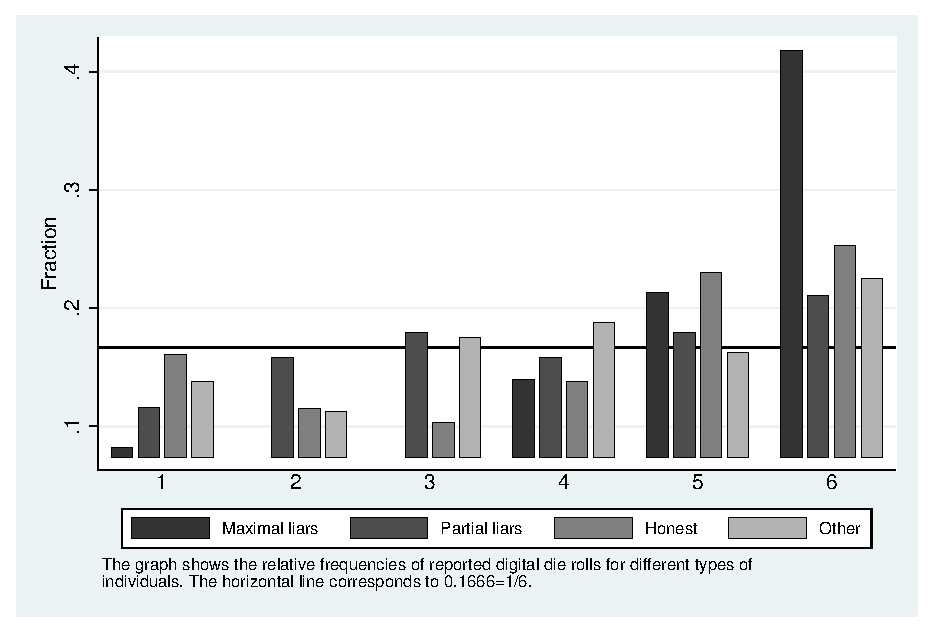
\includegraphics[scale=0.7]{ddie_type.eps}}
\caption{Lying and the digital die roll result. The graph shows relative frequencies of reported digital die rolls for different behavior types. The horizontal dashed line corresponds to $0.1666 = 1/6$. }\label{fig:digdietoss}
\end{figure}

\begin{table}[h!]
\begin{center}
\begin{tabular}{lcccc}
\hline\hline
  &Maximal lie&Partial lie &Honest&Total  \\
  \hline\hline
Always declare 0\% & 25 & 4 & 27 & 56 \\
Declare 0\% in at least 8 periods & 28 & 7 & 44 & 79   \\
  \hline\hline
Always declare above 0\%, but below 100\% & 1 & 0 & 25 & 26   \\
Declare above 0\%, but below 100\% in at least 8 periods & 7 & 8 & 53 & 68 \\
  \hline\hline
Always declare 100\% & 2 & 5 & 37 & 44 \\
Declare 100\% in a least 8 periods & 7 & 5 & 49 & 61 \\
                  \hline\hline
\multicolumn{5}{p{15cm}}{\tiny The table shows the frequency actions on the digital die task when 1, 2, 3, or 4 was rolled, depending on the individual's behavior in the main part of the experiment. }
\end{tabular}
\end{center}
\caption{Lying on the digital die task}\label{tab:digdie}

\end{table}


\begin{figure}
\begin{center}
	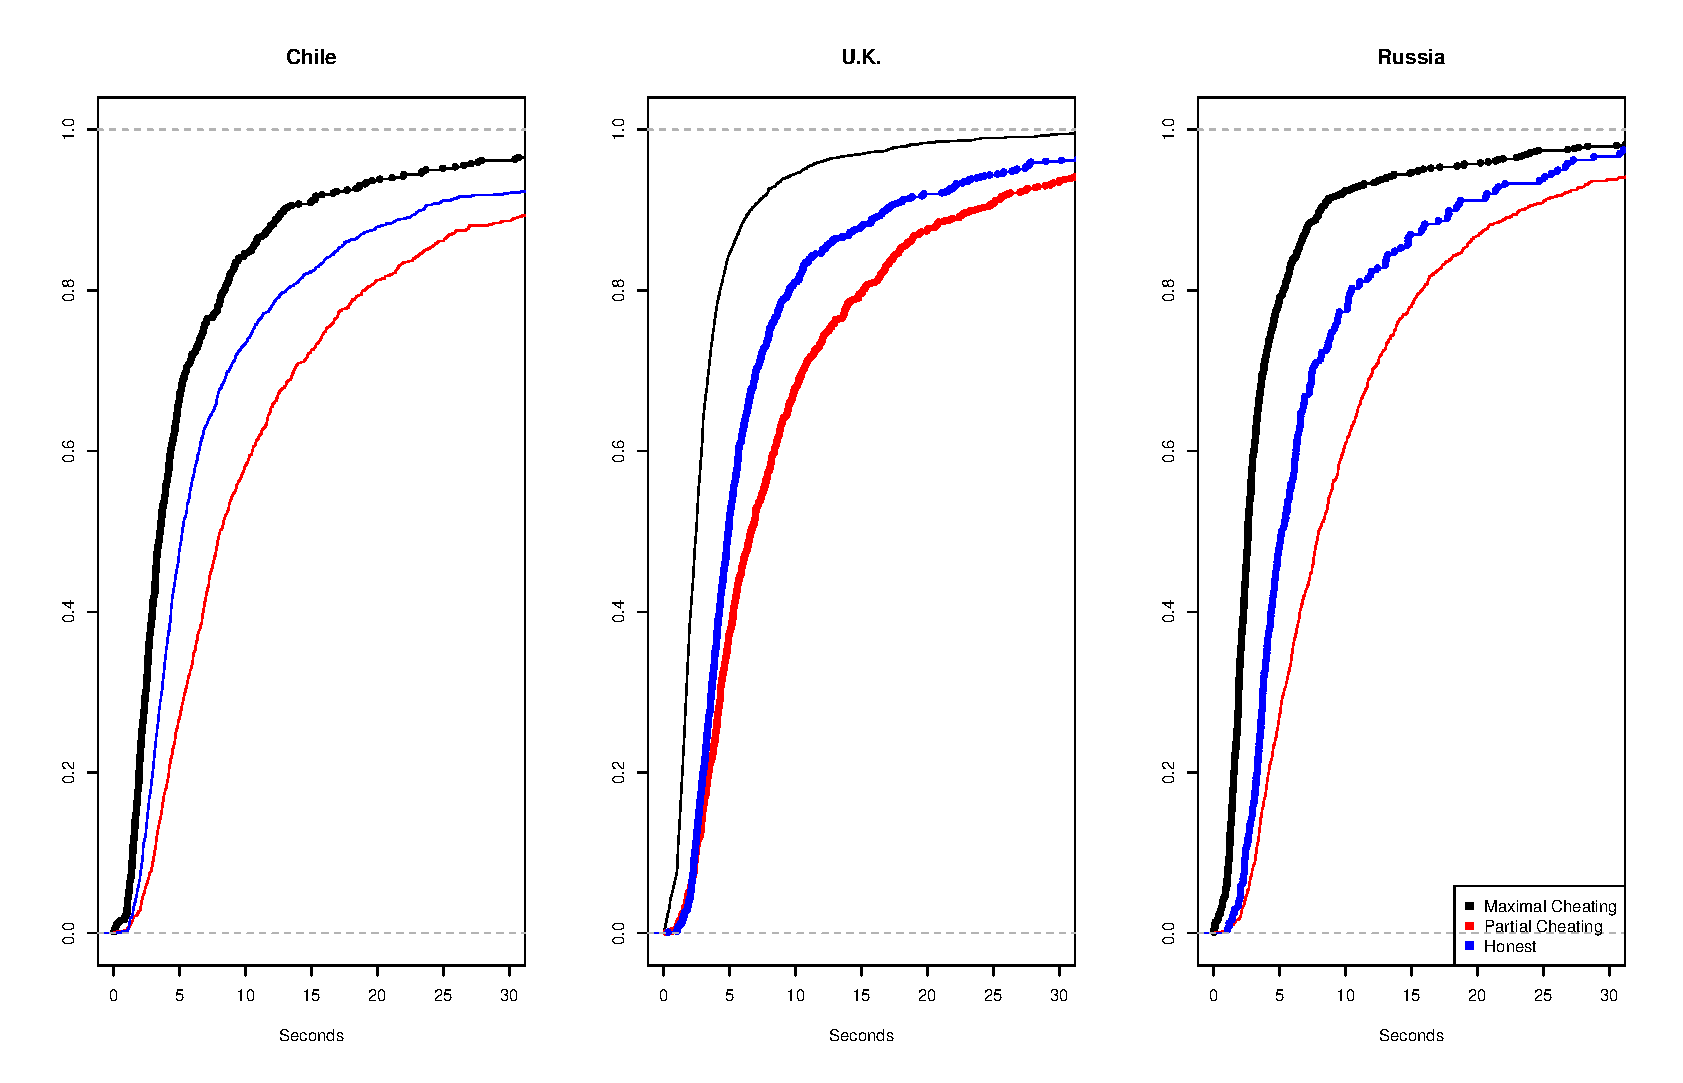
\includegraphics[scale=0.5]{RT_ECDF_countries.eps}
	
\end{center}	
	\caption{Distribution of reaction time by country. Figures present the cumulative distributions functions of TR for different decisions}
	\label{fig:response_country}
\end{figure}


\clearpage
\begin{table}[ht]
\begin{tabular}{p{15cm}c}
\hline \hline
Questions &  \\
\hline
``How often do you lend money to your friends. 0 - More often than once a week, 1 - Approximately once a week, 2 - Approximately once a month, 3 - Once a year or less often.''&0.626\\
``How often do you lend your belongings to your friends. 0 - More often than once a week, 1 - Approximately once a week, 2 - Approximately once a month, 3 - Once a year or less often.''&0.671\\
``How often do you leave your door open. 0 - Very often, 1 - Often, 3 - Sometimes, 4 - Rarely, 5 - Never.''&0.396\\
\hline \hline 
\footnotesize{The trusting behavior index is calculated as the normalized first principle component of 3 questions. The first principle component explained 44\% of variation.}

\end{tabular}
\caption{Components of the trusting behavior index. }
\label{tab:trust}
\end{table}

\begin{table}[ht]
\scriptsize
\begin{center}
{
\def\sym#1{\ifmmode^{#1}\else\(^{#1}\)\fi}
\begin{tabular}{p{10cm}*{2}{cc}}
\hline\hline
                &\multicolumn{2}{c}{Average} &\multicolumn{2}{c}{Per round}\\
\hline
Male            &    1.402\sym{***}&  (0.310)&    1.429\sym{***}&  (0.304)\\
Age             &  -0.0281         & (0.0417)&  -0.0283         & (0.0429)\\
Period          &                  &         &    0.165\sym{***}& (0.0165)\\
DG=0            &    0.230         &  (0.463)&    0.245         &  (0.452)\\
DG above 0      & -0.00228\sym{**} &(0.000936)& -0.00235\sym{**} &(0.000921)\\
Deduction 20\%  &    0.445         &  (0.327)&    0.493         &  (0.321)\\
Deduction 30\%  &   0.0118         &  (0.466)&  -0.0483         &  (0.453)\\
Shock           &    0.320         &  (0.453)&    0.515         &  (0.479)\\
L.Shock=Yes     &                  &         &   -0.411         &  (0.265)\\
Status          &    0.698         &  (0.597)&    0.801         &  (0.566)\\
Status, 200 ECU &  -0.0503         &  (0.796)&   -0.142         &  (0.770)\\
Non-fixed       &    1.165\sym{***}&  (0.432)&    1.240\sym{***}&  (0.425)\\
L.Dec. others, 1000&                  &         &   -0.191\sym{*}  &  (0.112)\\
Norms           &    0.244         &  (0.150)&    0.256\sym{*}  &  (0.146)\\
Trusting behavior index&   0.0802         &  (0.164)&   0.0827         &  (0.160)\\
SafeChoices     &   0.0743         & (0.0841)&   0.0606         & (0.0811)\\
Ideology        &  -0.0961         & (0.0769)&  -0.0842         & (0.0737)\\
Income          &   -0.563         &  (0.807)&   -0.644         &  (0.786)\\
Constant        &    11.55\sym{***}&  (1.227)&    11.00\sym{***}&  (1.232)\\
\hline
Observations    &      256         &         &     2304         &         \\
\(R^{2}\)       &    0.171         &         &    0.152         &         \\
\hline\hline
\multicolumn{5}{p{17cm}}{\tiny OLS regressions. Dependent variable is average performance over 10 rounds in the first model, and performance in a round for the second model. Robust standard errors for first model, standard errors clustered by subject for the second model. DG frac is the fraction of the 1000 ECU donated in the dictator game. Norms is the social norms index (see Table \ref{tab:norms}). SafeChoices if the number (0-10) of safe choices on the lottery task. Trusting behavior is the trusting behavior index (see Table \ref{tab:trust}). Income is the number of the individual's income bracket, rescaled between 0 and 1 (for Chile and the UK), and the individual's perceived income decile, rescaled between 0 and 1 (for Russia).}\\
\multicolumn{5}{l}{\footnotesize \sym{*} \(p<0.10\), \sym{**} \(p<0.05\), \sym{***} \(p<0.01\)}\\
\end{tabular}
}

\end{center}
\caption{Determinants of subject's performance, Russia.}
\label{table_ret_russia}
\end{table}
\clearpage

\begin{table}[ht]
\begin{center}
\scriptsize
{
\def\sym#1{\ifmmode^{#1}\else\(^{#1}\)\fi}
\begin{tabular}{l*{3}{cc}}
\hline\hline
                &\multicolumn{2}{c}{Model 1} &\multicolumn{2}{c}{Model 2} &\multicolumn{2}{c}{Model 3} \\
\hline
RET rank        &   -0.510\sym{***}& (0.0591)&   -0.314\sym{***}& (0.0497)&   -0.309\sym{***}& (0.0492)\\
RET deviation   &   0.0279\sym{***}&(0.00432)&   0.0258\sym{***}&(0.00428)&   0.0277\sym{***}&(0.00403)\\
Male            &  0.00712         & (0.0328)&   0.0830\sym{***}& (0.0264)&   0.0795\sym{***}& (0.0260)\\
Age             &  0.00799\sym{***}&(0.00264)&  0.00421\sym{*}  &(0.00250)&  0.00406         &(0.00254)\\
Period          &   -0.158\sym{***}&(0.00278)&   -0.146\sym{***}&(0.00274)&  -0.0955\sym{***}&(0.00276)\\
DG frac         &    0.582\sym{***}& (0.0801)&    0.167\sym{**} & (0.0662)&    0.146\sym{**} & (0.0656)\\
Deduction 20\%  &    0.108\sym{***}& (0.0378)&   0.0739\sym{**} & (0.0310)&   0.0738\sym{**} & (0.0304)\\
Deduction 30\%  &  -0.0443         & (0.0402)&  -0.0270         & (0.0323)&  -0.0296         & (0.0317)\\
Deduction 40\%  &    0.257\sym{**} &  (0.103)&    0.215\sym{***}& (0.0761)&    0.205\sym{***}& (0.0743)\\
Deduction 50\%  &   -0.168\sym{*}  & (0.0960)&  -0.0884         & (0.0827)&  -0.0985         & (0.0792)\\
Redistribution  &  -0.0371         & (0.0643)&   0.0325         & (0.0507)&   0.0300         & (0.0493)\\
Shock           &    0.163\sym{***}& (0.0581)&    0.162\sym{***}& (0.0482)&    0.150\sym{***}& (0.0465)\\
Shock, yes      &    0.356\sym{***}& (0.0465)&    0.336\sym{***}& (0.0441)&    0.348\sym{***}& (0.0398)\\
Status          &   -0.109         & (0.0677)&  -0.0744         & (0.0538)&  -0.0802         & (0.0526)\\
Status, 200 ECU &    0.132         & (0.0862)&    0.103         & (0.0670)&    0.113\sym{*}  & (0.0655)\\
Non-fixed       &   0.0887\sym{**} & (0.0432)&    0.118\sym{***}& (0.0354)&    0.117\sym{***}& (0.0347)\\
Russia          &   -0.129\sym{***}& (0.0501)&   -0.134\sym{***}& (0.0418)&   -0.150\sym{***}& (0.0413)\\
UK              &   -0.515\sym{***}& (0.0417)&   -0.323\sym{***}& (0.0357)&   -0.317\sym{***}& (0.0351)\\
Maximal lie this period&                  &         &    0.486\sym{***}& (0.0347)&                  &         \\
Partial lie this period&                  &         &    0.835\sym{***}& (0.0323)&                  &         \\
Maximal lie in period 1&                  &         &                  &         &    0.412\sym{***}& (0.0597)\\
Partial lie in period 1&                  &         &                  &         &    1.275\sym{***}& (0.0481)\\
Honest in period 1&                  &         &                  &         &    0.979\sym{***}& (0.0561)\\
Max. lie this and previous period&                  &         &                  &         &   -0.459\sym{***}& (0.0376)\\
Max. lie prev. period, part. lie this period&                  &         &                  &         &    0.510\sym{***}& (0.0648)\\
Max. lie prev. period, honest this period&                  &         &                  &         &    0.411\sym{***}& (0.0936)\\
Part. lie prev. period, max. lie this period&                  &         &                  &         &  -0.0159         & (0.0564)\\
Part. lie this and previous period&                  &         &                  &         &    0.401\sym{***}& (0.0365)\\
Part. lie prev. period, honest this period&                  &         &                  &         &    0.349\sym{***}& (0.0498)\\
Honest prev. period, max. lie this period&                  &         &                  &         &  -0.0422         & (0.0709)\\
Honest prev. period, part. lie this period&                  &         &                  &         &    0.499\sym{***}& (0.0537)\\
Constant        &    2.507\sym{***}& (0.0961)&    2.014\sym{***}& (0.0891)&    2.087\sym{***}& (0.0872)\\
\hline
Observations    &    10714         &         &    10714         &         &    10714         &         \\
\hline\hline
\multicolumn{7}{l}{\footnotesize OLS regression. Dependent variable is log reaction time. Standard errors are clustered by subject. Baseline category for subject decision in Model 2 is honest behavior in this period. Baseline category for subject decision in Model 3 is honest behavior in this and previous period.}\\
\multicolumn{7}{l}{\footnotesize \sym{*} \(p<0.10\), \sym{**} \(p<0.05\), \sym{***} \(p<0.01\)}\\
\end{tabular}
}

\end{center}
\caption{Determinants of reaction time}
\label{table_rt}
\end{table}

\clearpage

\begin{table}[ht]
\tiny
\begin{center}
\def\sym#1{\ifmmode^{#1}\else\(^{#1}\)\fi}
\begin{tabular}{|ll|cccccccccc|}
\hline\hline
&&1-1 ECU&1-10 ECU&1-20 ECU&1-30 ECU&1-40 ECU&1-50 ECU&1-60 ECU&1-70 ECU&1-80 ECU&1-90 ECU\\
\hline
&Low& 0.892857& 0.892857& 0.892857& 0.892857& 0.892857& 0.892857& 0.892857& 0.892857& 0.892857& 0.892857\\
Chile&High& 0.768831& 0.768831& 0.768831& 0.768831& 0.768831& 0.768831& 0.768831& 0.768831& 0.768831& 0.768831\\
&p& 0.000000& 0.000000& 0.000000& 0.000000& 0.000000& 0.000000& 0.000000& 0.000000& 0.000000& 0.000000\\
\hline&Low& 0.727344& 0.727344& 0.727344& 0.727344& 0.727344& 0.727344& 0.727344& 0.727344& 0.727344& 0.727344\\
Russia&High& 0.521875& 0.521875& 0.521875& 0.521875& 0.521875& 0.521875& 0.521875& 0.521875& 0.521875& 0.521875\\
&p& 0.000000& 0.000000& 0.000000& 0.000000& 0.000000& 0.000000& 0.000000& 0.000000& 0.000000& 0.000000\\
\hline&Low& 0.556693& 0.556693& 0.556693& 0.556693& 0.556693& 0.556693& 0.556693& 0.556693& 0.556693& 0.556693\\
UK&High& 0.266929& 0.266929& 0.266929& 0.266929& 0.266929& 0.266929& 0.266929& 0.266929& 0.266929& 0.266929\\
&p& 0.000000& 0.000000& 0.000000& 0.000000& 0.000000& 0.000000& 0.000000& 0.000000& 0.000000& 0.000000\\
\hline\multicolumn{11}{p{15cm}}{\tiny For each country, the first two rows report the frequencies of declarations for two groups of subjects. The third row reports the p-value for Fisher's exact test comparing these two frequencies.}\\
\end{tabular}
\end{center}
\caption{Near-maximal cheating depending on performance ($p$-values for two-sided Fisher's exact test).}
 \label{table:nearmax}
\end{table}

\begin{table}[ht]
\tiny
\begin{center}
\def\sym#1{\ifmmode^{#1}\else\(^{#1}\)\fi}
\begin{tabular}{|ll|cccccccccc|}
\hline\hline
&&1-1 ECU&1-10 ECU&1-20 ECU&1-30 ECU&1-40 ECU&1-50 ECU&1-60 ECU&1-70 ECU&1-80 ECU&1-90 ECU\\
\hline
&Female&   0.0103&   0.0301&   0.0327&   0.0391&   0.0423&   0.0590&   0.0673&   0.0673&   0.0699&   0.0705\\
Chile&Male&   0.0099&   0.0230&   0.0257&   0.0283&   0.0289&   0.0355&   0.0368&   0.0375&   0.0414&   0.0441\\
&p&   0.9512&   0.5498&   0.5752&   0.4207&   0.3315&   0.1554&   0.0856&   0.0926&   0.1185&   0.1549\\
\hline&Female&   0.0138&   0.0618&   0.0797&   0.0837&   0.0837&   0.1130&   0.1130&   0.1146&   0.1163&   0.1179\\
Russia&Male&   0.0068&   0.0301&   0.0323&   0.0331&   0.0346&   0.0541&   0.0586&   0.0586&   0.0586&   0.0602\\
&p&   0.2327&   0.0792&   0.0208&   0.0162&   0.0198&   0.0170&   0.0304&   0.0258&   0.0232&   0.0253\\
\hline&Female&   0.0095&   0.0387&   0.0539&   0.0630&   0.0642&   0.0765&   0.0770&   0.0770&   0.0778&   0.0782\\
UK&Male&   0.0083&   0.0279&   0.0340&   0.0351&   0.0377&   0.0411&   0.0419&   0.0423&   0.0426&   0.0434\\
&p&   0.8392&   0.3686&   0.1583&   0.0628&   0.0860&   0.0318&   0.0343&   0.0365&   0.0350&   0.0377\\
\hline\multicolumn{11}{p{15cm}}{\tiny For each country, the first two rows report the frequencies of declarations for two groups of subjects. The third row reports the p-value for the OLS regression where the dependent variable is 0 or 1 (if there is near-maximal cheating), and the independent variable is the dummy the subject group, and standard errors are clustered by subject. }\\
\end{tabular}
\end{center}
\caption{Near-maximal cheating depending on gender ($p$-values for two-sided Fisher's exact test). }
 \label{table:nearmax_male}
\end{table}

\begin{table}[ht]
\tiny
\begin{center}
\def\sym#1{\ifmmode^{#1}\else\(^{#1}\)\fi}
\begin{tabular}{|ll|cccccccccc|}
\hline\hline
&&1-1 ECU&1-10 ECU&1-20 ECU&1-30 ECU&1-40 ECU&1-50 ECU&1-60 ECU&1-70 ECU&1-80 ECU&1-90 ECU\\
\hline
&DG>0& 0.855782& 0.855782& 0.855782& 0.855782& 0.855782& 0.855782& 0.855782& 0.855782& 0.855782& 0.855782\\
Chile&DG=0& 0.307143& 0.307143& 0.307143& 0.307143& 0.307143& 0.307143& 0.307143& 0.307143& 0.307143& 0.307143\\
&p& 0.000000& 0.000000& 0.000000& 0.000000& 0.000000& 0.000000& 0.000000& 0.000000& 0.000000& 0.000000\\
\hline&DG>0& 0.735897& 0.735897& 0.735897& 0.735897& 0.735897& 0.735897& 0.735897& 0.735897& 0.735897& 0.735897\\
Russia&DG=0& 0.268852& 0.268852& 0.268852& 0.268852& 0.268852& 0.268852& 0.268852& 0.268852& 0.268852& 0.268852\\
&p& 0.000000& 0.000000& 0.000000& 0.000000& 0.000000& 0.000000& 0.000000& 0.000000& 0.000000& 0.000000\\
\hline&DG>0& 0.555587& 0.555587& 0.555587& 0.555587& 0.555587& 0.555587& 0.555587& 0.555587& 0.555587& 0.555587\\
UK&DG=0& 0.096226& 0.096226& 0.096226& 0.096226& 0.096226& 0.096226& 0.096226& 0.096226& 0.096226& 0.096226\\
&p& 0.000000& 0.000000& 0.000000& 0.000000& 0.000000& 0.000000& 0.000000& 0.000000& 0.000000& 0.000000\\
\hline\multicolumn{11}{p{15cm}}{\tiny For each country, the first two rows report the frequencies of declarations for two groups of subjects. The third row reports the p-value for Fisher's exact test comparing these two frequencies.}\\
\end{tabular}
\end{center}
\caption{Near-maximal cheating depending on DG donation ($p$-values for two-sided Fisher's exact test). }
 \label{table:nearmax_dg}
\end{table}

\begin{comment}
\section{Cheating game with audit}


\begin{table}[h!]
\caption{Distribution of Cheating Behavior with 10\% Audit Rate}\label{heuristic}
\begin{center}
\begin{tabular}{lccccc}
\hline\hline
  & Chile & Russia & U.K. &  Total  \\
  \hline\hline
Always declare 0\% & 7.0 & 19.9 & 29.6 & 10.0 \\
Declare 0\% in at least 8 rounds & 10.6 & 32.1 & 37.5 & 22.0   \\
  \hline\hline
Always declare above 0\%, but below 100\% & 14.8 & 17.3 & 15.9 & 15.8   \\
Declare above 0\%, but below 100\% in at least 8 rounds & 24.2 & 28.9 & 22.7 & 25.4 \\
  \hline\hline
Always declare 100\% & 37.5 & 14.1 & 20.5 & 27.2 \\
Declare 100\% in a least 8 rounds & 45.3 & 15.4 & 25.0 & 32.4 \\
                  \hline\hline
\end{tabular}
\end{center}
\end{table}

\begin{figure}[!htb]
\centerline{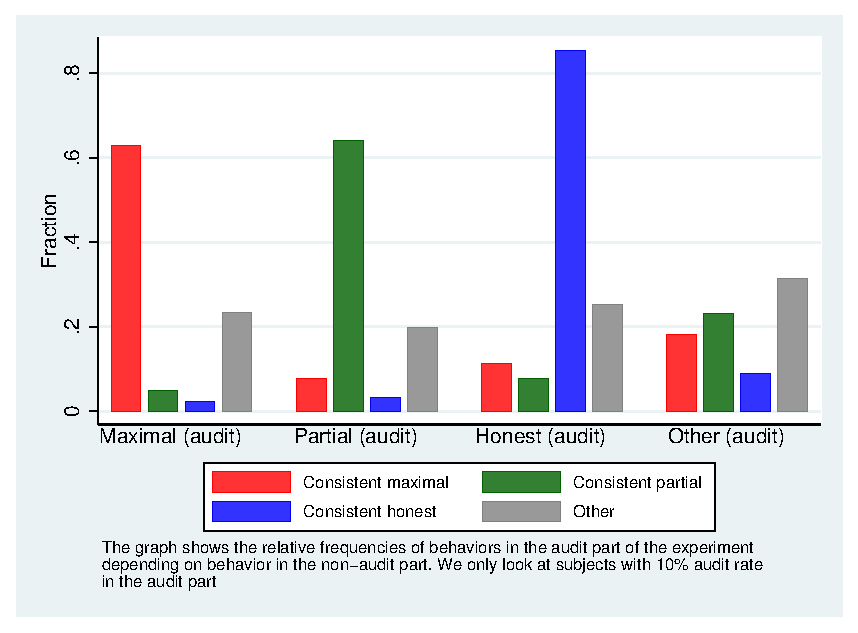
\includegraphics{audit_type.eps}}
\caption{Cheating Behavior in Main and Audit parts of the Experiment. }\label{fig:audit}
\end{figure}

\begin{table}[ht]
\begin{center}
\tiny
\def\sym#1{\ifmmode^{#1}\else\(^{#1}\)\fi}
\begin{tabular}{l|cccccc|cc}
\hline\hline
&\multicolumn{6}{c|}{\bf All\space{}countries}&\multicolumn{2}{c}{\bf All\space{}countries}\\ &\multicolumn{6}{c|}{Mlogit, average marginal effects }&\multicolumn{2}{c}{OLS}\\
                &\multicolumn{2}{c}{Maximal lying}&\multicolumn{2}{c}{Partial lying}&\multicolumn{2}{c}{Honest}  &\multicolumn{2}{c}{Partial lying}\\
\hline
ncorrect\_ranka  &   0.0798         & (0.0543)&  -0.0832         & (0.0634)&  0.00339         & (0.0669)&   0.0830         & (0.0952)\\
ncorrect\_dev3   & -0.00617\sym{*}  &(0.00341)&  0.00668\sym{*}  &(0.00376)&-0.000512         &(0.00404)&  0.00259         &(0.00497)\\
Male            &   0.0806\sym{**} & (0.0325)&  -0.0982\sym{***}& (0.0368)&   0.0176         & (0.0375)&   0.0592         & (0.0523)\\
Age             & -0.00790\sym{**} &(0.00313)&  0.00184         &(0.00340)&  0.00607\sym{*}  &(0.00356)&  0.00325         &(0.00621)\\
period4         &  0.00472\sym{***}&(0.00150)& -0.00456\sym{***}&(0.00176)&-0.000156         &(0.00168)& -0.00481\sym{*}  &(0.00253)\\
DG=0          &    0.149\sym{*}  & (0.0785)&   -0.181\sym{***}& (0.0537)&   0.0314         & (0.0825)&    0.157\sym{*}  & (0.0929)\\
DG frac         &   -0.398\sym{***}&  (0.126)&   -0.101         &  (0.107)&    0.499\sym{***}&  (0.124)&   0.0760         &  (0.172)\\
Deduction 20\%&  -0.0391         & (0.0374)&  -0.0141         & (0.0436)&   0.0531         & (0.0458)&    0.109\sym{*}  & (0.0633)\\
Deduction 30\%&   0.0547         & (0.0401)&  -0.0117         & (0.0422)&  -0.0430         & (0.0438)&   0.0734         & (0.0627)\\
Shock         &  0.00481         & (0.0609)&   -0.134\sym{**} & (0.0601)&    0.130\sym{*}  & (0.0711)&    0.131\sym{*}  & (0.0759)\\
Shock, yes    &  0.00898         & (0.0273)&   0.0366         & (0.0353)&  -0.0456         & (0.0330)&   0.0422         & (0.0489)\\
Status        &  -0.0567         & (0.0693)&  -0.0316         & (0.0755)&   0.0883         & (0.0819)&    0.138\sym{*}  & (0.0824)\\
Status, 200 ECU&  -0.0476         & (0.0673)&  0.00764         & (0.0746)&   0.0400         & (0.0812)&   0.0497         & (0.0925)\\
Non-fixed     &   0.0373         & (0.0597)&  -0.0839         & (0.0621)&   0.0467         & (0.0620)&    0.206\sym{***}& (0.0704)\\
Russia        &   0.0932\sym{**} & (0.0406)&    0.102\sym{**} & (0.0453)&   -0.195\sym{***}& (0.0415)&  -0.0233         & (0.0599)\\
UK            &    0.159\sym{***}& (0.0555)&  0.00191         & (0.0547)&   -0.161\sym{***}& (0.0517)&   -0.129         & (0.0813)\\
Constant        &                  &         &                  &         &                  &         &   0.0692         &  (0.192)\\
\hline
Observations    &     4920         &         &     4920         &         &     4920         &         &     1188         &         \\
D20=D30         &   0.0139         &         &    0.958         &         &   0.0346         &         &    0.568         &         \\
Russia=UK       &    0.304         &         &    0.131         &         &    0.595         &         &    0.252         &         \\
\hline\hline
\multicolumn{9}{p{16cm}}{\tiny The first three columns report average marginal effects for multinomial logistic regression (dependent variable is whether the subject declared 0\%, 100\%, or something in between, in a given round). Standard errors are clustered by subject. The fourth column reports OLS regression, the dependent variable is the fraction of income declared in a given round. We only include subjects who partially cheated in at least 8 rounds, and declarations strictly between 0\% and 100\%. Standard errors are clustered by subject. RET rank is the national rank, between 0 and 1, of subject's national performance at the real effort task. RET Deviation is the difference between actual number of correct additions and one predicted from subject and period FE. DG frac is the fraction of the 1000 ECU donated in the dictator game.}\\
\multicolumn{9}{l}{\tiny \sym{*} \(p<0.1\), \sym{**} \(p<0.05\), \sym{***} \(p<0.01\)}\\
\end{tabular}
\end{center}
\caption{Determinants of lying in each period, 10\% audit rate}
\label{table2_audit10}
\end{table}


\clearpage
\begin{table}[ht]
\begin{center}
\tiny
\def\sym#1{\ifmmode^{#1}\else\(^{#1}\)\fi}
\begin{tabular}{l|cccccc|cc}
\hline\hline
&\multicolumn{6}{c|}{\bf Chile}&\multicolumn{2}{c}{\bf Chile}\\ &\multicolumn{6}{c|}{Mlogit, average marginal effects }&\multicolumn{2}{c}{OLS}\\
                &\multicolumn{2}{c}{Maximal lying}&\multicolumn{2}{c}{Partial lying}&\multicolumn{2}{c}{Honest}  &\multicolumn{2}{c}{Partial lying}\\
\hline
ncorrect\_ranka  &    0.125\sym{*}  & (0.0695)&   -0.216\sym{**} & (0.0892)&   0.0910         & (0.0996)&   -0.272\sym{*}  &  (0.148)\\
ncorrect\_dev3   & -0.00579         &(0.00451)&   0.0145\sym{**} &(0.00570)& -0.00873         &(0.00637)&  0.00939         &(0.00813)\\
Male            &   0.0751\sym{*}  & (0.0441)&  -0.0163         & (0.0537)&  -0.0587         & (0.0590)&   0.0655         & (0.0710)\\
Age             &-0.000694         &(0.00273)& -0.00535         &(0.00430)&  0.00604         &(0.00516)& -0.00202         &(0.00905)\\
period4         &  0.00272         &(0.00194)& -0.00149         &(0.00226)& -0.00124         &(0.00229)& -0.00180         &(0.00343)\\
DG=0          &    0.134         &  (0.129)&   -0.134         &  (0.111)& 0.000310         &  (0.157)&   0.0977         &  (0.170)\\
DG frac         &   -0.214         &  (0.150)&   -0.207         &  (0.142)&    0.421\sym{**} &  (0.175)&    0.167         &  (0.284)\\
Deduction 20\%&  -0.0584         & (0.0453)&  -0.0594         & (0.0573)&    0.118\sym{*}  & (0.0656)&    0.182\sym{*}  & (0.0917)\\
Deduction 30\%&   0.0515         & (0.0452)&  -0.0628         & (0.0572)&   0.0113         & (0.0635)&    0.169\sym{*}  & (0.0887)\\
Shock         &  -0.0527         & (0.0655)&  -0.0469         & (0.0881)&   0.0997         & (0.0983)&    0.197\sym{*}  &  (0.102)\\
Shock, yes    &   0.0249         & (0.0509)&   0.0458         & (0.0516)&  -0.0707         & (0.0578)&   0.0533         & (0.0640)\\
Status        &  -0.0606         & (0.0758)&  -0.0378         &  (0.101)&   0.0985         &  (0.114)&    0.226\sym{**} & (0.0955)\\
Status, 200 ECU&   0.0189         &  (0.101)&  -0.0600         & (0.0994)&   0.0411         &  (0.124)& -0.00396         &  (0.160)\\
Non-fixed     &   0.0379         & (0.0645)&  -0.0878         & (0.0742)&   0.0498         & (0.0815)&    0.213\sym{**} & (0.0971)\\
Constant        &                  &         &                  &         &                  &         &    0.196         &  (0.266)\\
\hline
Observations    &     2480         &         &     2480         &         &     2480         &         &      575         &         \\
D20=D30         &   0.0156         &         &    0.955         &         &    0.112         &         &    0.906         &         \\
\hline\hline
&\multicolumn{6}{c|}{\bf Russia}&\multicolumn{2}{c}{\bf Russia}\\ &\multicolumn{6}{c|}{Mlogit, average marginal effects }&\multicolumn{2}{c}{OLS}\\
                &\multicolumn{2}{c}{Maximal lying}&\multicolumn{2}{c}{Partial lying}&\multicolumn{2}{c}{Honest}  &\multicolumn{2}{c}{Partial lying}\\
\hline
ncorrect\_ranka  &  -0.0836         &  (0.107)&    0.122         &  (0.110)&  -0.0383         &  (0.104)&    0.251\sym{*}  &  (0.129)\\
ncorrect\_dev3   & -0.00179         &(0.00612)&  0.00342         &(0.00605)& -0.00163         &(0.00606)&  0.00377         &(0.00688)\\
Male            &   0.0952         & (0.0602)&   -0.161\sym{***}& (0.0614)&   0.0663         & (0.0547)&   0.0563         & (0.0878)\\
Age             &  -0.0167         & (0.0150)&  0.00366         & (0.0126)&   0.0130         & (0.0102)&  0.00399         & (0.0271)\\
period4         &   0.0126\sym{***}&(0.00306)&  -0.0116\sym{***}&(0.00367)&-0.000961         &(0.00341)&  -0.0111\sym{**} &(0.00482)\\
DG=0          &   0.0939         &  (0.102)&   -0.260\sym{***}& (0.0804)&    0.166         &  (0.103)&    0.174         &  (0.118)\\
DG frac         &   -0.724\sym{***}&  (0.213)&   0.0335         &  (0.199)&    0.691\sym{***}&  (0.192)&  -0.0233         &  (0.241)\\
Deduction 20\%&  -0.0245         & (0.0732)&   0.0753         & (0.0733)&  -0.0508         & (0.0632)&  -0.0787         &  (0.105)\\
Deduction 30\%&  -0.0166         & (0.0808)&    0.128\sym{*}  & (0.0761)&   -0.112\sym{*}  & (0.0672)&   -0.130         &  (0.114)\\
Shock         & -0.00202         &  (0.105)&   -0.159         &  (0.108)&    0.161         &  (0.101)&   0.0409         &  (0.106)\\
Shock, yes    & -0.00187         & (0.0382)&   0.0253         & (0.0412)&  -0.0234         & (0.0340)&  -0.0105         & (0.0505)\\
Status        &  -0.0805         &  (0.121)&  0.00834         &  (0.128)&   0.0722         &  (0.110)&   0.0501         &  (0.127)\\
Status, 200 ECU&   -0.117         & (0.0965)&   0.0750         &  (0.112)&   0.0419         &  (0.104)&   0.0573         & (0.0910)\\
Non-fixed     &  -0.0167         &  (0.114)&   0.0201         &  (0.115)& -0.00336         & (0.0996)&    0.137         &  (0.135)\\
Constant        &                  &         &                  &         &                  &         &    0.237         &  (0.554)\\
\hline
Observations    &     1560         &         &     1560         &         &     1560         &         &      423         &         \\
D20=D30         &    0.912         &         &    0.485         &         &    0.369         &         &    0.631         &         \\
\hline\hline
&\multicolumn{6}{c|}{\bf UK}&\multicolumn{2}{c}{\bf UK}\\ &\multicolumn{6}{c|}{Mlogit, average marginal effects }&\multicolumn{2}{c}{OLS}\\
                &\multicolumn{2}{c}{Maximal lying}&\multicolumn{2}{c}{Partial lying}&\multicolumn{2}{c}{Honest}  &\multicolumn{2}{c}{Partial lying}\\
\hline
ncorrect\_ranka  &    0.235\sym{*}  &  (0.134)&  -0.0797         &  (0.150)&   -0.156         &  (0.173)&    0.660\sym{***}&  (0.108)\\
ncorrect\_dev3   &  -0.0138         &(0.00884)& -0.00641         &(0.00712)&   0.0202\sym{**} &(0.00795)&  -0.0129\sym{*}  &(0.00707)\\
Male            &   0.0814         & (0.0861)&   -0.196\sym{**} & (0.0842)&    0.114         & (0.0837)&    0.134         &  (0.103)\\
Age             &  -0.0135\sym{*}  &(0.00708)&  0.00856         &(0.00632)&  0.00492         &(0.00666)&  0.00980\sym{**} &(0.00370)\\
period4         & -0.00353         &(0.00309)& -0.00106         &(0.00367)&  0.00460         &(0.00319)&  0.00123         &(0.00236)\\
DG=0          &    0.367\sym{*}  &  (0.219)&   -0.175         &  (0.148)&   -0.192         &  (0.147)&    0.319\sym{***}&  (0.109)\\
DG frac         &   -0.115         &  (0.400)&  -0.0461         &  (0.256)&    0.161         &  (0.272)&    0.606\sym{**} &  (0.225)\\
Deduction 20\%&  -0.0628         & (0.0848)&   0.0414         &  (0.126)&   0.0214         &  (0.128)&    0.505\sym{***}&  (0.112)\\
Deduction 30\%&    0.204         &  (0.128)&   -0.122         & (0.0981)&  -0.0827         &  (0.113)&    0.188\sym{***}& (0.0566)\\
Constant        &                  &         &                  &         &                  &         &   -0.595\sym{***}&  (0.160)\\
\hline
Observations    &      880         &         &      880         &         &      880         &         &      190         &         \\
D20=D30         &   0.0575         &         &    0.269         &         &    0.504         &         &  0.00392         &         \\
\hline\hline
\multicolumn{9}{p{16cm}}{\tiny The first three columns report average marginal effects for multinomial logistic regression (dependent variable is whether the subject declared 0\%, 100\%, or something in between, in a given round). Standard errors are clustered by subject. The fourth column reports OLS regression, the dependent variable is the fraction of income declared in a given round. We only include subjects who partially cheated in at least 8 rounds, and declarations strictly between 0\% and 100\%. Standard errors are clustered by subject. RET rank is the national rank, between 0 and 1, of subject's national performance at the real effort task. RET Deviation is the difference between actual number of correct additions and one predicted from subject and period FE. DG frac is the fraction of the 1000 ECU donated in the dictator game.}\\
\multicolumn{9}{l}{\tiny \sym{*} \(p<0.1\), \sym{**} \(p<0.05\), \sym{***} \(p<0.01\)}\\
\end{tabular}
\end{center}
\caption{Determinants of lying in each period, by country, 10\% audit rate}
\label{table2_audit10_country}
\end{table}
\end{comment}
\end{document}

